%%%%%%%%%%%%%%%%%%%%%%%%%%%%%%%%%%%%%%%%%
% Masters/Doctoral Thesis 
% LaTeX Template
% Version 2.1 (2/9/15)
%
% This template has been downloaded from:
% http://www.LaTeXTemplates.com
%
% Version 2.0 major modifications by:
% Vel (vel@latextemplates.com)
%
% Original authors:
% Steven Gunn  (http://users.ecs.soton.ac.uk/srg/softwaretools/document/templates/)
% Sunil Patel (http://www.sunilpatel.co.uk/thesis-template/)
%
% License:
% CC BY-NC-SA 3.0 (http://creativecommons.org/licenses/by-nc-sa/3.0/)
%
%%%%%%%%%%%%%%%%%%%%%%%%%%%%%%%%%%%%%%%%%

%------------------------------------------------------------------------------
%	PACKAGES AND OTHER DOCUMENT CONFIGURATIONS
%------------------------------------------------------------------------------

\documentclass[
11pt, % The default document font size, options: 10pt, 11pt, 12pt
%oneside, % Two side (alternating margins) for binding by default, uncomment to switch to one side
english, % ngerman for German
onehalfspacing %singlespacing, % Single line spacing, alternatives: onehalfspacing or doublespacing
%draft, % Uncomment to enable draft mode (no pictures, no links, overfull hboxes indicated)
%nolistspacing, % If the document is onehalfspacing or doublespacing, uncomment this to set spacing in lists to single
%liststotoc, % Uncomment to add the list of figures/tables/etc to the table of contents
%toctotoc, % Uncomment to add the main table of contents to the table of contents
%parskip, % Uncomment to add space between paragraphs
]{MastersDoctoralThesis} % The class file specifying the document structure

\usepackage[utf8]{inputenc} % Required for inputting international characters
\usepackage[T1]{fontenc} % Output font encoding for international characters

\usepackage{palatino} % Use the Palatino font by default

%\usepackage[backend=bibtex,style=trad-unsrt,sorting=nyt,natbib=true,isbn=false,doi=false,url=false]{biblatex} % User the bibtex backend with the authoryear citation style (which resembles APA)
%\addbibresource{C2_preliminaries.bib} % The filename of the bibliography
%\addbibresource{C3_turbulence.bib} % The filename of the bibliography
%\addbibresource{C4_RB_VMS.bib} % The filename of the bibliography
%\addbibresource{C5_TBT_OSS.bib} % The filename of the bibliography
%\addbibresource{C6_SRK.bib} % The filename of the bibliography
%\addbibresource{C7_SVMS.bib} % The filename of the bibliography
%\addbibresource{C8_NACA.bib} % The filename of the bibliography
\bibliographystyle{abbrv}

\usepackage[]{csquotes} % Required to generate language-dependent quotes in the bibliography

\usepackage{amssymb,amsmath}
\usepackage{amsfonts}
\usepackage{subfigure}
\usepackage{multirow}
\usepackage[table]{xcolor}
\usepackage{pifont}
\usepackage{amsthm}
\usepackage{tabularx}
\usepackage{multirow}
\usepackage{multicol}
\usepackage[ruled,vlined]{algorithm2e}
\usepackage{algpseudocode}
%------------------------------------------------------------------------------
%	INCLUDE DEFINITIONS FILE
%------------------------------------------------------------------------------
% Mathematic enviroments
\newtheorem{theorem}{Theorem}
\newtheorem{lemma}[theorem]{Lemma}
\newtheorem{corollary}[theorem]{Corollary}
\newtheorem{remark}{Remark}
\newtheorem{definition}{Definition}

%Article 1
\def\half{\frac{1}{2}}
\def\boxeq#1{\frame{\parbox{\textwidth}{#1}}} 
\def\Eq#1{(\ref{eq-#1})}
\def\Lem#1{\ref{lem-#1}}
\def\Fig#1{\ref{fig-#1}}
\def\x{x}
\def\cl{ \nonumber \\}
\def\el{\nonumber}
\def\jumpl{\lbrack\!\lbrack}
\def\jumpr{\rbrack\!\rbrack}
\def\jump#1{\jumpl #1 \jumpr}
\def\jumpt#1{\underline{\jump{#1}}}
\def\mean#1{\{\! \!\{ #1\}\! \!\}}
\def\meanpv#1{\{ #1\}}
\def\meanhar#1{\langle#1\rangle}
\def\Qq{ \Omega \times (0,t^*)}
%\def\mean#1{\left\{\hskip -5pt\left\{#1\right\}\hskip -5pt\right\}}
%\def\smean#1{\{\hskip -3pt\{#1\}\hskip -3pt\}}
\def\jumpl{\lbrack\!\lbrack}
\def\jumpr{\rbrack\!\rbrack}
\def\jump#1{\jumpl #1 \jumpr}
\def\vhk{V^k_{h,0}}%{\mathcal{V}_h^k}
\def\vhkperp{(V^k_{h,0})^\perp}%{\mathcal{V}_h^k}
\def\vh1{V_{h}^1}%{\mathcal{V}_h^1}
\def\osc{\textrm{osc}(\infty)}
\def\smear{\textrm{smear}(\infty)}
\def\osctwo{\textrm{osc}(2)}
\def\smeartwo{\textrm{smear}(2)}
\def\pe{\textrm{Pe}}
\def\thn{\mathcal{T}_h}
\def\thm{\mathcal{T}_m}
\def\th{\mathcal{T}_h}
\def\tint#1{\int_0^{t^*} #1 {\rm d}t}
\def\szpp{\kappa_h^\perp}%{\Pi_{SZ}^\perp}
\def\sno#1{\tint{\| \delta^\frac{1}{2} \bb \cdot \szpp (\nabla  #1) \|^2 }}
\def\tno#1{\| #1 \|(T) + \sno{#1}}
\def\szp{\kappa_h}%{\Pi_{SZ}}
\def\lp{\pi_{h}}
\def\lpp{\pi_{h}^\perp}
\def\nop{\Pi_{nod}}
\def\nopp{\Pi_{nod}^\perp}
\def\bb{\beta}

%Article 2
\def\half{\frac{1}{2}}
\def\boxeq#1{\frame{\parbox{\textwidth}{#1}}} 
\def\Eq#1{(\ref{eq-#1})}
\def\Lem#1{(\ref{lem-#1})}
\def\Fig#1{Fig. \ref{fig-#1}}
\def\x{x}
\def\cl{ \nonumber \\}
\def\el{\nonumber}
\def\jumpl{\lbrack\!\lbrack}
\def\jumpr{\rbrack\!\rbrack}
\def\jump#1{\jumpl #1 \jumpr}
\def\jumpt#1{\underline{\jump{#1}}}
\def\mean#1{\{\! \!\{ #1\}\! \!\}}
\def\meanpv#1{\{ #1\}}
\def\meanhar#1{\langle#1\rangle}
\def\avg#1{\left\langle #1 \right\rangle}
\def\jumpl{\lbrack\!\lbrack}
\def\jumpr{\rbrack\!\rbrack}
\def\jump#1{\jumpl #1 \jumpr}
\def\vh{V_h}
\def\osc{\textrm{osc}(\infty)}
\def\smear{\textrm{smear}(\infty)}
\def\osctwo{\textrm{osc}(2)}
\def\smeartwo{\textrm{smear}(2)}
\def\pe{\textrm{Pe}}
\def\nh{\mathcal{N}_h}
\def\tint#1{\displaystyle\int_0^T #1 {\rm d}t}
\def\szpp{\kappa_h^\perp}%{\Pi_{SZ}^\perp}
\def\sno#1{\tint{\| \delta^\frac{1}{2} \bb \cdot \szpp (\nabla  #1) \|^2 }}
\def\tno#1{\| #1 \|(T) + \sno{#1}}
\def\szp{\kappa_h}%{\Pi_{SZ}}
\def\lp{\pi_{h}}
\def\lpp{\pi_{h}^\perp}
\def\nop{\Pi_{nod}}
\def\nopp{\Pi_{nod}^\perp}
\def\bb{\beta}
\def\infno#1#2{\| #1 \|_{L^\infty(#2)}}
\def\infnok#1{\infno{#1}{K}}
\def\sgn#1{\textrm{sign}(#1)}
\def\half{\frac{1}{2}}
\def\boxeq#1{\frame{\parbox{\textwidth}{#1}}} 
\def\Eq#1{(\ref{eq-#1})}
\def\Lem#1{(\ref{lem-#1})}
\def\Fig#1{Fig. \ref{fig-#1}}
\def\x{x}
\def\cl{ \nonumber \\}
\def\el{\nonumber}
\def\jumpl{\lbrack\!\lbrack}
\def\jumpr{\rbrack\!\rbrack}
\def\jump#1{\jumpl #1 \jumpr}
\def\jumpt#1{\underline{\jump{#1}}}
\def\mean#1{\{\! \!\{ #1\}\! \!\}}
\def\meanpv#1{\{ #1\}}
\def\meanhar#1{\langle#1\rangle}
\def\avg#1{\left\langle #1 \right\rangle}
\def\jumpl{\lbrack\!\lbrack}
\def\jumpr{\rbrack\!\rbrack}
\def\jump#1{\jumpl #1 \jumpr}
\def\vh{V_h}
\def\osc{\textrm{osc}(\infty)}
\def\smear{\textrm{smear}(\infty)}
\def\osctwo{\textrm{osc}(2)}
\def\smeartwo{\textrm{smear}(2)}
\def\pe{\textrm{Pe}}
\def\nh{\mathcal{N}_h}
\def\tint#1{\displaystyle\int_0^T #1 {\rm d}t}
\def\szpp{\kappa_h^\perp}%{\Pi_{SZ}^\perp}
\def\sno#1{\tint{\| \delta^\frac{1}{2} \bb \cdot \szpp (\nabla  #1) \|^2 }}
\def\tno#1{\| #1 \|(T) + \sno{#1}}
\def\szp{\kappa_h}%{\Pi_{SZ}}
\def\lp{\pi_{h}}
\def\lpp{\pi_{h}^\perp}
\def\nop{\Pi_{nod}}
\def\nopp{\Pi_{nod}^\perp}
\def\bb{\beta}
\def\infno#1#2{\| #1 \|_{L^\infty(#2)}}
\def\infnok#1{\infno{#1}{K}}
\def\sgn#1{\textrm{sign}(#1)}

%Paper 3		
\def\comment#1{{\color{red} #1}}
\def\ahierro#1{{\color{blue} #1}}
\def\pkus#1{{\color{green} #1}}
\def\half{\frac{1}{2}}
\def\boxeq#1{\frame{\parbox{\textwidth}{#1}}} 
\def\Eq#1{(\ref{eq-#1})}
\def\Lem#1{(\ref{lem-#1})}
\def\Fig#1{Fig. \ref{fig-#1}}
\def\Alg#1{Alg. \ref{alg-#1}}
\def\x{x}
\def\cl{ \nonumber \\}
\def\el{\nonumber}
\def\jumpl{\lbrack\!\lbrack}
\def\jumpr{\rbrack\!\rbrack}
\def\jump#1{\jumpl #1 \jumpr}
\def\jumpt#1{\underline{\jump{#1}}}
\def\mean#1{\{\! \!\{ #1\}\! \!\}}
\def\meanpv#1{\{ #1\}}
\def\meanhar#1{\langle#1\rangle}
\def\avg#1{\left\langle #1 \right\rangle}

\def\jumpl{\lbrack\!\lbrack}
\def\jumpr{\rbrack\!\rbrack}
\def\jump#1{\jumpl #1 \jumpr}
\def\vmk{V_{m,0}}
\def\vmkperp{V_{m,0}^\perp}
\def\vm1{V_{m}^1}
\def\vm{V_m}
\def\v#1{V_{#1}}
\def\osc{\textrm{osc}(\infty)}
\def\smear{\textrm{smear}(\infty)}
\def\osctwo{\textrm{osc}(2)}
\def\smeartwo{\textrm{smear}(2)}
\def\pe{\textrm{Pe}}
\def\nh{\mathcal{N}_h}
\def\tint#1{\displaystyle\int_0^T #1 {\rm d}t}
\def\szpp{\kappa_h^\perp}
\def\sno#1{\tint{\| \delta^\frac{1}{2} \bb \cdot \szpp (\nabla  #1) \|^2 }}
\def\tno#1{\| #1 \|(T) + \sno{#1}}
\def\szp{\kappa_h}
\def\lp{\pi_{h}}
\def\lpp{\pi_{h}^\perp}
\def\nop{\Pi_{nod}}
\def\nopp{\Pi_{nod}^\perp}
\def\bb{\beta}
\def\infno#1#2{\| #1 \|_{L^\infty(#2)}}
\def\infnok#1{\infno{#1}{K}}
\def\sgn#1{\textrm{sign}(#1)}
\def\aperr{\eta}
\def\aperrmk{\aperr_m^i}
\def\prerr{E}
\def\prerrmk{E_m^i}
\def\mesh#1{\mathcal{T}_{#1}}
\def\meshm{\mesh{m}}
\def\faces#1{\mathcal{F}_{#1}}
\def\facesm{\faces{m}}
\def\grad{\mathcal{G}}
\def\gradmk{\grad_m^i}
\def\prgrad{{G}}
\def\prgradmk{\prgrad_m^i}
\def\shockf{\mathcal{S}}
\def\shockfmk{\shockf_m^i}
\def\reff{\mathcal{R}}
\def\reffmk{\reff_m^i}
\def\refp{\mathcal{P}}
\def\refpmk{\refp_m^i}
\def\damp{\omega}
\def\dampmk{\damp_k}
\def\maxdamp{\damp_{\max}}
\def\mindamp{\damp_{\min}}
\def\adiff{\varepsilon}
\def\setfaces{\mathcal{E}_m}
\def\setintfaces{\mathcal{E}_m^0}
\def\nelem{N^{\rm el}_m}
\def\pnelem{N^{\rm el}_{m-1}}
\def\elem{{K_i}}
\def\refidfunction#1{F_{#1}}
\def\prevID{{F{m}(i)}}
\def\numchilds{n_c}
\DeclareMathOperator*{\argmax}{arg\,max}
\def\noteSB#1{{\color{red}**** #1 ****}}	

% New commands
\def\facet{F}

%------------------------------------------------------------------------------
%	THESIS INFORMATION
%------------------------------------------------------------------------------

\thesistitle{Gradient Jump Viscosity Shock Capturing Techniques} % Your thesis title, this is used in the title and abstract, print it elsewhere with \ttitle
\supervisor{Prof. Santiago \textsc{Badia}} % Your supervisor's name, this is used in the title page, print it elsewhere with \supname
\examiner{} % Your examiner's name, this is not currently used anywhere in the template, print it elsewhere with \examname
\degree{Doctor of Philosophy} % Your degree name, this is used in the title page and abstract, print it elsewhere with \degreename
\author{Alba \textsc{Hierro Fabregat}} % Your name, this is used in the title page and abstract, print it elsewhere with \authorname
\addresses{} % Your address, this is not currently used anywhere in the template, print it elsewhere with \addressname

\subject{} % Your subject area, this is not currently used anywhere in the template, print it elsewhere with \subjectname
\keywords{} % Keywords for your thesis, this is not currently used anywhere in the template, print it elsewhere with \keywordnames
\university{\href{http://www.upc.edu}{Universitat Politècnica de Catalunya}} % Your university's name and URL, this is used in the title page and abstract, print it elsewhere with \univname
\program{Doctorat en Matemàtica Aplicada}
\department{Departament d'Enginyeria Civil i Ambiental} % Your department's name and URL, this is used in the title page and abstract, print it elsewhere with \deptname
\group{} %{\href{http://www.cimne.com/spacehome/2/1156}{Large Scale Scientific Computing group}} % Your research group's name and URL, this is used in the title page, print it elsewhere with \groupname
\faculty{\href{https://www.fme.upc.edu}{Facultat de Matemàtiques i Estadística}} % Your faculty's name and URL, this is used in the title page and abstract, print it elsewhere with \facname

\hypersetup{pdftitle=\ttitle} % Set the PDF's title to your title
\hypersetup{pdfauthor=\authorname} % Set the PDF's author to your name
\hypersetup{pdfkeywords=\keywordnames} % Set the PDF's keywords to your keywords

\begin{document}

\frontmatter % Use roman page numbering style (i, ii, iii, iv...) for the pre-content pages

\pagestyle{plain} % Default to the plain heading style until the thesis style is called for the body content

%------------------------------------------------------------------------------
%	TITLE PAGE
%------------------------------------------------------------------------------

\begin{titlepage}
\begin{center}

\textsc{\LARGE \univname}\\[1.5cm] % University name
\textsc{\Large Doctoral Thesis}\\[0.5cm] % Thesis type

\HRule \\[0.4cm] % Horizontal line
{\huge \bfseries \ttitle}\\[0.4cm] % Thesis title
\HRule \\[1.5cm] % Horizontal line
 
\begin{minipage}{0.4\textwidth}
\begin{flushleft} \large
\emph{Author:}\\
%\href{http://www.johnsmith.com}{\authorname} % Author name - remove the \href bracket to remove the link
{\authorname} % Author name - remove the \href bracket to remove the link
\end{flushleft}
\end{minipage}
\begin{minipage}{0.4\textwidth}
\begin{flushright} \large
\emph{Supervisor:} \\
%\href{http://www.jamessmith.com}{\supname} % Supervisor name - remove the \href bracket to remove the link  
{\supname} % Supervisor name - remove the \href bracket to remove the link  
\end{flushright}
\end{minipage}\\[3cm]
 
\large \textit{A thesis submitted in fulfilment of the requirements\\ for the degree of \degreename}\\[0.3cm] % University requirement text
\textit{in the}\\[0.4cm]
%\groupname\\\deptname\\[2cm] % Research group name and department name
\progname\\[0.5cm]
\deptname\\[2cm] % Research group name and department name 
 
{\large Barcelona, February 2016}\\[2cm] % Date+

\includegraphics[width=8cm]{../Figures/Cover/logo_fme.png}
%\includegraphics{Logo} % University/department logo - uncomment to place it
 
\vfill
\end{center}
\end{titlepage}

%------------------------------------------------------------------------------
%	DEDICATION
%------------------------------------------------------------------------------

\dedicatory{To \ldots} 

%------------------------------------------------------------------------------
%	DECLARATION PAGE
%------------------------------------------------------------------------------

%\begin{declaration}
%\addchaptertocentry{\authorshipname}
%
%\noindent I, \authorname, declare that this thesis titled, \enquote{\ttitle} and the work presented in it are my own. I confirm that:
%
%\begin{itemize} 
%\item This work was done wholly or mainly while in candidature for a research degree at this University.
%\item Where any part of this thesis has previously been submitted for a degree or any other qualification at this University or any other institution, this has been clearly stated.
%\item Where I have consulted the published work of others, this is always clearly attributed.
%\item Where I have quoted from the work of others, the source is always given. With the exception of such quotations, this thesis is entirely my own work.
%\item I have acknowledged all main sources of help.
%\item Where the thesis is based on work done by myself jointly with others, I have made clear exactly what was done by others and what I have contributed myself.\\
%\end{itemize}
% 
%\noindent Signed:\\
%\rule[0.5em]{25em}{0.5pt} % This prints a line for the signature
% 
%\noindent Date:\\
%\rule[0.5em]{25em}{0.5pt} % This prints a line to write the date
%\end{declaration}
%
\cleardoublepage

%------------------------------------------------------------------------------
%	QUOTATION PAGE
%------------------------------------------------------------------------------

\vspace*{0.2\textheight}

%\noindent\enquote{\itshape Thanks to my solid academic training, today I can write hundreds of words on virtually any topic without possessing a shred of information, which is how I got a good job in journalism.}\bigbreak
%
%\hfill Dave Barry

\noindent\enquote{\itshape La teoria sense pràctica és inútil
Però la pràctica sense teoria, és efímera.}\bigbreak

\hfill Brigitte Vasallo

\noindent\enquote{\itshape Understand well as I may, my comprehension can only be an infinitesimal fraction of all I want to understand.}

\hfill Ada Lovelace


%------------------------------------------------------------------------------
%	ABSTRACT PAGE
%------------------------------------------------------------------------------

\begin{abstract}
\addchaptertocentry{\abstractname} % Add the abstract to the table of contents

%The Thesis Abstract is written here (and usually kept to just this page). The page is kept centered vertically so can expand into the blank space above the title too\ldots
%\input{abstract}

\end{abstract}

%------------------------------------------------------------------------------
%	RESUM
%------------------------------------------------------------------------------

\begin{resum}
\addchaptertocentry{\resumname} % Add the abstract to the table of contents

%\input{resum}

\end{resum}

%------------------------------------------------------------------------------
%	ACKNOWLEDGEMENTS
%------------------------------------------------------------------------------

\begin{acknowledgements}
\addchaptertocentry{\acknowledgementname} % Add the acknowledgements to the table of contents

Filipos
JIPI
Marta i Iris

La tesi que teniu a les mans s'ha escrit en uns anys crucials de creixement personal que, si bé no es pot apreciar en el contingut explícit d'aquestes pàgines, s'ha anat consolidant en paralel i per a mi resulta impossible pensar en tota aquesta investigació sense tenir en compte tots els projectes que l'han acompanyat en el temps i les persones que n'han format part. Vull tenir per a algunes d'elles també unes paraules de gratitud.\\


Recordo com si fos ahir l'Uri enumerant-me la llista d'avantatges d'emprendre una carrera acadèmica que mai abans m'havia plantejat. Si no fos per aquelles paraules d'anims, aquesta tesi no hauria ni començat a caminar.

Un no esstà mai sol quan empren un projecte, hi ha molts moments i persones que directa o indirectament també han col·laborat a dirigir el rumb d'aquestes pàgines.

Hi ha persones que han estat sempre allà. Estaven abans, m'han acompanyat durant i espero que segueixin al meu costat per molts anys més. Amics com els Kàxeros de Tortosa que sempre estan allà, especialment Quim que ha fet molts cops les corbes del Garraf per a venir a dinar en mi a Castelldefels o Marta i Vane que m'han tret tantes vegades a sopar i a plorar i riure de les nostres desgràcies. Amigues com la Txela que m'ha acompanyat a la fi del món i a la vegada que ha sabut fer, amb l'Ana, de casa seua parada i fonda de menjar macarrons els diumenges per començar amb ganes la setmana el dilluns següent. Tota la gent del Dinar del Mes que apareixen ja en els agraïments de tantes tesis que podríem obrir una consultoria d'acompanyament a doctorands en crisis (Ei! Idea d'empresa!).

També hi ha gent que ha anat apareixent al llarg dels darrers 5 anys i que si bé no han

Desde 2015 hay un poquito de Guatemala en mí, de la cosmovisión indígena de quienes nos acogieron en sus casas, dels Quetzals Rebeldes que em van acompanyar en aquesta aventura y, sobretodo, de la gente bonita de la Plataforma de Barcelona que ha sabido recogerme, levantarme y abrazarme, ponerle la piel necesaria, a este \'utimo año de doctorado.
%The acknowledgements and the people to thank go here, don't forget to include your project advisor\ldots
%\input{acknowledgements}

\end{acknowledgements}

%------------------------------------------------------------------------------
%	LIST OF CONTENTS/FIGURES/TABLES PAGES
%------------------------------------------------------------------------------

\tableofcontents % Prints the main table of contents

\listoffigures % Prints the list of figures

\listoftables % Prints the list of tables

%------------------------------------------------------------------------------
%	ABBREVIATIONS
%------------------------------------------------------------------------------

\begin{abbreviations}%{ll} % Include a list of abbreviations (a table of two columns)
\textbf{BC} & \textbf{B}oundary \textbf{C}onditions \\
\textbf{bGJV} & \textbf{b}oundary \textbf{G}radient \textbf{J}ump \textbf{V}iscosity\\
\textbf{CFL} & \textbf{C}ourant-\textbf{F}riederich-\textbf{L}evy (condition)\\
\textbf{cG} & \textbf{C}ontinuous \textbf{G}alerkin \\
\textbf{CDR} & \textbf{C}onvection \textbf{D}iffusion \textbf{R}eaction (equation)\\
\textbf{dG} & \textbf{D}iscontinuous \textbf{G}alerkin \\
\textbf{DMP} & \textbf{D}iscrete \textbf{M}aximum \textbf{P}rinciple \\
\textbf{EV} & \textbf{E}ntropy \textbf{V}iscosity\\
\textbf{FE} & \textbf{F}inite \textbf{E}lement \\
\textbf{FV} & \textbf{F}initie \textbf{V}olumes \\
\textbf{GJV} & \textbf{G}radient \textbf{J}ump \textbf{V}iscosity\\
\textbf{GLS} & \textbf{G}alerkin \textbf{L}east \textbf{S}quares \\
\textbf{LED} & \textbf{L}ocal \textbf{E}xtremum \textbf{D}iminishing\\
\textbf{LPS} & \textbf{L}ocal \textbf{P}rojection \textbf{S}tabilization\\
\textbf{nGJV} & \textbf{n}odal \textbf{G}radient \textbf{J}ump \textbf{V}iscosity\\
\textbf{NPS} & \textbf{N}odal \textbf{P}rojection \textbf{Stabilization}\\
\textbf{RV} & \textbf{R}esidual-based \textbf{Viscosity}\\
\textbf{SUPG} & \textbf{S}treamline \textbf{U}pwind \textbf{P}etrov-\textbf{G}alerkin\\
\textbf{TVD} & \textbf{T}otal \textbf{V}ariation \textbf{D}iminishing\\
\textbf{VMS} & \textbf{V}ariational \textbf{M}ulti\textbf{S}cales\\
\textbf{wNPS} & \textbf{w}eighted \textbf{N}odal \textbf{P}rojection \textbf{Stabilization}\\
\end{abbreviations}

%------------------------------------------------------------------------------
%	PHYSICAL CONSTANTS/OTHER DEFINITIONS
%------------------------------------------------------------------------------

%\begin{constants}%{lr@{${}={}$}l} % The list of physical constants is a three column table
%
% %The \SI{}{} command is provided by the siunitx package, see its documentation for instructions on how to use it
%
%Speed of Light & $c$ & \SI{2.99792458e8}{\meter\per\second} (exact)\\
%%Constant Name & $Symbol$ & $Constant Value$ with units\\
%
%\end{constants}

%------------------------------------------------------------------------------
%	SYMBOLS
%------------------------------------------------------------------------------

\begin{symbols}

\multicolumn{3}{c}{{\Large \textbf{Lower-case Roman}}}\\
$d$ & space dimension\\
$n$ & unit outside normal\\
$u(\x,t)$      & variable of interest       &  \\

\addlinespace % Gap to separate the Roman lower from Roman Capital
\addlinespace

\multicolumn{3}{c}{{\Large \textbf{Upper-case Roman}}}\\
\addlinespace % Gap to separate the Roman lower from Roman Capital
\addlinespace

\multicolumn{3}{c}{{\Large \textbf{Lower-case Greek}}}\\
$\beta$ & convection term\\
$ \tau_c $ & continuity stabilization parameter & \\

\addlinespace % Gap to separate the Greek lower symbols from the Greek Capital
\addlinespace

\multicolumn{3}{c}{{\Large \textbf{Upper-case Greek}}}\\
$\Omega$ & domain \\
$\Gamma$  & domain boundary ($\Gamma=\partial\Omega$) & \\
$\Gamma_{\rm in}$ & inflow boundary ($\Gamma_{\rm in} := \{ x \in \partial \Omega: \, \beta(x) \cdot n(x) < 0\}$)\\
\addlinespace % Gap to separate the Greek capital symbols from the subscripts
\addlinespace

\multicolumn{3}{c}{{\Large \textbf{Superscripts and subscripts}}}\\
$ (\cdot)_h $ & Finite Element component & \\
$ (\cdot)_{n+1} $ & current time step & \\
$ (\cdot)_n $ & previous time step & \\

\end{symbols}

%------------------------------------------------------------------------------
%	THESIS CONTENT - CHAPTERS
%------------------------------------------------------------------------------

\mainmatter % Begin numeric (1,2,3...) page numbering

\pagestyle{thesis} % Return the page headers back to the "thesis" style

% Include the chapters of the thesis as separate files from the Chapters folder
% Uncomment the lines as you write the chapters

\chapter{Introduction and Motivation}
\label{chap-intro}


How to deal with the shocks. In the {author's} masther thesis \ref{masterthesis}, it can be appreciated how some very different shock capturing techniques perform with diferent methods, continuous and discontinuous Galerkin with low and high order. The test were performed for one-dimensional cases but they already shed light some how effective some of these techniques were in different paradigms.

One important revelation was that, contrary to what was expected, the discontinuous Galerkin techniques were not more effective in capturing the discontinuities than the continuous method. This was due to the fact that the interior penalty terms would not let the method to capture a pure discontinuity between two elements and this induce spurious oscillations around the discontinuity or sharp layer.

In \ref{masterthesis} the Gradient Jump Viscosity (GJV) method was already introduced for the one-dimensional case as an adaptation of the method proposed by \cite{burman_nonlinear_2007} for the Burgers' equation.

\section{Structure of the document}
Chapters \ref{chap-paper1}, \ref{chap-paper2} and \ref{chap-paper3} are based on the \comment{author's} articles \cite{badia_stabilized_2012}, \cite{badia_discrete_2015} and \cite{paper3} respectively. The three chapters follow the structure of the publications and, thus, are selfcontained. Some of the notation used might slightly differ from one chapter to another according to the necessities of each analysis. In this sense, on \ref{chap-paper3}, the elements of the mesh are ordered while in the rest they are not, and there is some abuse of notation on the solution space: it is called $\thn$ trough the document but it stnds for different concretizations in each of them (continuous or discontinuous). 

\section{Things}
On the continuous Galerkin paradigm, the need of an extra linear stabilization seems to be obvious and the challenge faced in \ref{chap-paper1} will be how to blend the linear and nonlinear stabilization in such a way that one preserves the DMP property. The discontinuous Galerkin, on the other hand, do already have implicit linear stabilization in its definition so the artificial viscosity can be directly applied on the top of it.

The origin of continuous and discontinuous Galerkin. The amount of work related to the development of methods that enjoy the DMP for cG in comparison with dG. In this sense we feel that the present work is a remarkable contribution to the field since it includes methods that go from the analysis of the possible artificial diffusion techniques that would enjoy such properties to the implementation of graphviscosity methods that allow the method to stricly fulfil the property for any kind of underlying mesh.

In all of the cases a gradient jump viscosity shock detectors are implemented. The definition of those detectors can be generalized and applied either for continuous and discontinuous methods. This property is very interesting specially for hybrid meshes such as the continuous-discontinuous Galerkin method introduced in \cite{badia_adaptive_2013} for dealing with hanging nodes in adaptive meshes. In this sense, in chapter \ref{chap-paper3}, there is a possible approach to deal with the adaptive paradigm.

The present thesis aims to be the first compilation of different applications that take use of the Gradient Jump Viscosity shock detectors in order to implement Discrete Maximum Principle enjoying methods.

\section{Intro paper 1}

The finite element (FE) Galerkin approximation of convection-dominated and transport problems
with non-smooth data produces highly oscillatory results, and additional numerical stabilization must be
introduced. The most rudimentary stabilization methods add non-consistent terms, e.g., homogeneous artificial diffusion and upwinding techniques \cite{von_neumann_method_1950}. 
The SUPG method originally proposed in \cite{brooks_streamline_1982} was the first consistent stabilization technique, 
allowing for higher order approximations. Since this groundbreaking
work, the amount of research produced on linear stabilization has been impressive, leading to a wide 
variety of formulations (see, e.g., \cite{hughes_variational_1998,codina_finite_1997,becker_finite_2001,guermond_stabilization_1999}). 
%Remarkable works are the concept of subgrid stabilization in \cite{}, the variational
%multiscale paradigm in \cite{hughes_variational_1998} or the symmetric projection stabilization techniques in \cite{codina_finite_1997,becker_finite_2001}.

We can roughly distinguish between linear stabilization methods based on FE residuals 
and methods based on projections. Residual-based methods include the
SUPG, GLS, and VMS formulations \cite{hughes_multiscale_1995,hughes_variational_1998} proposed by Hughes and co-workers. These
methods are consistent by definition and exhibit optimal convergence and stability properties.
However, these methods can be cumbersome for complex systems of equations, specially
in multiphysics \cite{planas_approximation_2011,badia_unconditionally_2013}, where the number of stabilization terms to be integrated 
notably increases; only some terms do introduce stability whereas the rest are only required
to keep consistency. These additional terms can couple unknowns that are uncoupled
at the con\-ti\-nuous level, destroy symmetric properties and  make unstable segregated
algorithms \cite{badia_unconditionally_2013}. Furthermore, the extension of these methods to transient problems is
involved unless space-time discretizations are considered \cite{codina_time_2007,burman_consistent_2010}. 


% Modify the sentece since the introduction
% In fact, for the sake of convergenge, only the projection orthogonal to the FE space is used.
In order to solve all these problems, symmetric projection stabilization only introduces the terms that are required for stability purposes. More specifically, it only provides stability of the projection orthogonal to the FE space, so that the stabilization terms do not spoil the convergence of the method. %Since the introduction of the whole quantities to be stabilized, e.g. the convective term, would spoil convergence, the projection of these quantities onto the corresponding FE space is subtracted.  
This way, we keep convergence and attain the desired stability, e.g., relying on continuous inf-sup conditions. The key aspect of these methods is the choice of the projector. One example  is the orthogonal subscales method in \cite{codina_stabilization_2000}, which uses a (global) $L^2$ projection. In order to avoid the need of a global projection, local projection stabilization techniques have been proposed, e.g., in \cite{braack_local_2006,matthies_unified_2007}. The resulting methods only involve local projections but are restricted to particular mesh topologies or require enriched FE spaces. A recent improvement of these formulations has been recently proposed in \cite{badia_stabilized_2012} for pressure stability of the Stokes problem, which makes use of  a particular Scott-Zhang projector which is local and does not require any particular type of mesh or FE space enrichment; this method has been named \emph{nodal projection stabilization} (NPS), due to the nodal-wise nature of the projection. A closely related term-by-term pressure/convection stabilization has been presented in \cite{rebollo_high_2013}. The main difference between the stabilization mechanism in \cite{badia_stabilized_2012} and  \cite{rebollo_high_2013} is the \emph{buffer} FE space in which the projections are performed. The buffer space in \cite{badia_stabilized_2012} is the same velocity FE space, whereas  it has one order less than the velocity space (assumed to be at least quadratic) in \cite{rebollo_high_2013}.

 %This method coincides with the nodal interpolation proposed by Chac\'on \textit{et al.} in \cite{rebollo_high_2013}.


Linear stabilization certainly reduces oscillations but still exhibits overshoots and undershoots around discontinuities or shocks. As a result, nonlinear stabilization techniques (traditionally called shock-capturing) have been designed, usually in the form of an artificial viscosity that depends on the solution (see, e.g., \cite{johnson_convergence_1987,johnson_convergence_1990,szepessy_convergence_1989}). This nonlinear viscosity must be active around shocks, where it sacrifices the order of accuracy of the method but improves stability. The way this artificial viscosity is computed leads to different families of methods. Most methods are based on residual-based viscosity \cite{codina_stabilization_2000,lube_residual-based_2006,john_spurious_2007,john_spurious_2008} combined with linear stabilization. Guermond and co-workers have proposed entropy-viscosity methods, %have recently been proposed by Guermond and co-workers,
 in which the nonlinear viscosity is defined in terms of some entropy inequality \cite{guermond_entropy_2011}. %Convergence analysis and monotonic properties of EV methods are an open problem.

The aim of the nonlinear stabilization is to eliminate oscillations around shocks, which implies to satisfy a discrete maximum principle (DMP). Only a few FE methods are known to satisfy some monotonicity property (see, e.g., \cite{mizukami_petrov-galerkin_1985,burman_nonlinear_2002,burman_stabilized_2005}). It is remarkable the work by Burman and Ern in \cite{burman_nonlinear_2002}, where they state the properties to be fulfilled by a method in order to satisfy a DMP property in a useful variational setting for nonlinear problems. The methods in \cite{burman_stabilized_2005,burman_edge_2004} satisfy a DMP property for the steady-state convection-diffusion-reaction (CDR) problem but it has been observed that they are too dissipative for practical use in \cite{john_spurious_2008} and the extension to time-dependent problems is unclear. Afterwards, Burman has proposed in \cite{burman_nonlinear_2007} a method which only includes nonlinear stabilization and satisfies monotonicity properties for the (transient) Burgers' problem in one dimension. %Another approach is the ??? method  by Kuzmin, %which essentially modifies the resulting matrix in order to attain the DMP property.  
Existence and uniqueness have been proved for some residual-based shock-capturing techniques combined with local
projection stabilization via Lipschitz continuity and Brouwer's fixed point theorem in \cite{barrenechea_local_2013}.

%the resulting method satisfies a DMP but it has been observed
%to be too dissipative for practical use in \cite{}. In \cite{}, 

\section{Intro paper 2}

As it was already exposed in the previous chapter, it is well known that the operator $L$ associated to an elliptic problem such as the convection-diffusion problem enjoys the maximum property, meaning that the maximum (resp., minimum) of the solution to the problem $Lu=f$ is achieved on the boundary of the domain if the source term, $f$, is negative (resp., positive). 
%Moreover, under certain extra regularity conditions, the operator enjoys the strong maximum principle meaning that the solution has no local maximum (resp., minimum) in the interior of the domain if $f\leq 0$ (resp., $f\geq 0$) .
In particular, this property ensures that the solution of the problem will not show oscillations. The solution of a convection-dominated problem may present sharp layers that may induce spurious oscillations in the discrete approximation of the solution. We are interested in finding a method that ensures a similar maximum property at the discrete discontinuous level in order to obtain a method that gives oscillation free solutions.

As we have previously explained, when the problem is discretized, this maximum property may be inherited by what is called \textit{discrete maximum principle} (DMP). Several definitions of the DMP have been proposed in the literature for continuous discrete approximations (see \cite{codina_discontinuity-capturing_1993,hohn_remarks_1981,varga_discrete_1966,burman_edge_2004,roos_robust_2008}). Some of them are equivalent while some others are weaker or stronger. There is also a lot of literature about the conditions on the mesh for the Poisson problem to enjoy the DMP \cite{hohn_remarks_1981,vejchodsky_discrete_2007,horvath_discrete_2013,payette_performance_2012} as well as discrete methods specially implemented to fulfil such property. Methods have been designed for linear finite differences \cite{ciarlet_discrete_1970} and continuous linear finite elements \cite{ciarlet_maximum_1973,codina_discontinuity-capturing_1993,mizukami_petrov-galerkin_1985,burman_discrete_2004,burman_edge_2004,burman_stabilized_2005}. {These methods are implicit in sense, and usually based on the addition of AV to the problem at hand; they are traditionally called shock (or discontinuity)-capturing techniques, even though we favour the notation \emph{nonlinear stabilization}.} 
%There is also a interesting simple approach to the problem given by Kreuzer \cite{kreuzer_note_2012} consisting on applying a simple cutoff to the solution but it can not be applied in an implicit code and moreover it only works when the maximum and the minimum of the problem are known beforehand. 
Some approaches to prove a DMP using piecewise higher order polynomials have been done \cite{nagarajan_enforcing_2011,payette_performance_2012,kuzmin_design_2008,vejchodsky_discrete_2007,vejchodsky_higher-order_2010,yanik_discrete_1987,yanik_sufficient_1989} but only the Poisson problem has been proved to enjoy the DMP and only on certain one-dimensional (1D) meshes \cite{vejchodsky_discrete_2007} and on very restrictive quadratic and cubic two dimensional meshes \cite{lorenz_zur_1977,hohn_remarks_1981}. When it comes to discontinuous methods, most of the shock capturing techniques are based on the concept of slope limiter, proposed by Cockburn and Shu for conservation laws \cite{cockburn_rungekutta_1998,cockburn_runge-kutta_1990} and latter adapted to the convection-dominated convection-diffusion problem  \cite{cockburn_rungekutta_2001}. The same strategy can be applied to finite volume methods (see \cite{zhang_maximum-principle-satisfying_2010,zhang_maximum-principle-satisfying_2011,zhang_maximum-principle-satisfying_2012}). Again, these methods consist in a postprocess after the solution is computed and are designed for explicit methods. {However, as far as we know, there are no works dealing with nonlinear stabilization and implicit DMP-preserving dG formulations. In fact, even the definition of what a DMP for dG means is open.}

Concerning to the study of the DMP for the Poisson problem in the dG setting, there is {only} one work by Horv\'ath and Mincsovics \cite{horvath_discrete_2013}; they analyse the fulfilment of certain condition on the stiffness matrix $\mathbf{K}$ that ensure the following property for the 1D interior penalty (IP) method:
\begin{align*}
\mathbf{Ku}\leq 0 \quad \Longrightarrow   \quad \max \mathbf{u} \leq \max\{0,\max \mathbf{u}_{\partial \Omega}\}. 
%\quad \forall u\in\mathbb{R}^{N_h}%\mathcal{C}^2({\Omega})\cap\mathcal{C}(\bar{\Omega}).
\end{align*} 

\chapter{Monotonicity preserving methods for continuous Galerkin method}
\label{chap-paper1}
\section{Introduction}\label{s-intro}
%
%In this work, we design stabilized finite element (FE) approximations of hyperbolic problems
%with monotonicity properties, which also serve to solve singular limits of 
%convection-diffusion-reaction problems. We focus on the linear tranport equation
%and the nonlinear Burgers equation.

The finite element (FE) Galerkin approximation of convection-dominated and transport problems
with non-smooth data produces highly oscillatory results, and additional numerical stabilization must be
introduced. The most rudimentary stabilization methods add non-consistent terms, e.g., homogeneous artificial diffusion and upwinding techniques \cite{von_neumann_method_1950}. 
The SUPG method originally proposed in \cite{brooks_streamline_1982} was the first consistent stabilization technique, 
allowing for higher order approximations. Since this groundbreaking
work, the amount of research produced on linear stabilization has been impressive, leading to a wide 
variety of formulations (see, e.g., \cite{hughes_variational_1998,codina_finite_1997,becker_finite_2001,guermond_stabilization_1999}). 
%Remarkable works are the concept of subgrid stabilization in \cite{}, the variational
%multiscale paradigm in \cite{hughes_variational_1998} or the symmetric projection stabilization techniques in \cite{codina_finite_1997,becker_finite_2001}.

We can roughly distinguish between linear stabilization methods based on FE residuals 
and methods based on projections. Residual-based methods include the
SUPG, GLS, and VMS formulations \cite{hughes_multiscale_1995,hughes_variational_1998} proposed by Hughes and co-workers. These
methods are consistent by definition and exhibit optimal convergence and stability properties.
However, these methods can be cumbersome for complex systems of equations, specially
in multiphysics \cite{planas_approximation_2011,badia_unconditionally_2013}, where the number of stabilization terms to be integrated 
notably increases; only some terms do introduce stability whereas the rest are only required
to keep consistency. These additional terms can couple unknowns that are uncoupled
at the con\-ti\-nuous level, destroy symmetric properties and  make unstable segregated
algorithms \cite{badia_unconditionally_2013}. Furthermore, the extension of these methods to transient problems is
involved unless space-time discretizations are considered \cite{codina_time_2007,burman_consistent_2010}. 


% Modify the sentece since the introduction
% In fact, for the sake of convergenge, only the projection orthogonal to the FE space is used.
In order to solve all these problems, symmetric projection stabilization only introduces the terms that are required for stability purposes. More specifically, it only provides stability of the projection orthogonal to the FE space, so that the stabilization terms do not spoil the convergence of the method. %Since the introduction of the whole quantities to be stabilized, e.g. the convective term, would spoil convergence, the projection of these quantities onto the corresponding FE space is subtracted.  
This way, we keep convergence and attain the desired stability, e.g., relying on continuous inf-sup conditions. The key aspect of these methods is the choice of the projector. One example  is the orthogonal subscales method in \cite{codina_stabilization_2000}, which uses a (global) $L^2$ projection. In order to avoid the need of a global projection, local projection stabilization techniques have been proposed, e.g., in \cite{braack_local_2006,matthies_unified_2007}. The resulting methods only involve local projections but are restricted to particular mesh topologies or require enriched FE spaces. A recent improvement of these formulations has been recently proposed in \cite{badia_stabilized_2012} for pressure stability of the Stokes problem, which makes use of  a particular Scott-Zhang projector which is local and does not require any particular type of mesh or FE space enrichment; this method has been named \emph{nodal projection stabilization} (NPS), due to the nodal-wise nature of the projection. A closely related term-by-term pressure/convection stabilization has been presented in \cite{rebollo_high_2013}. The main difference between the stabilization mechanism in \cite{badia_stabilized_2012} and  \cite{rebollo_high_2013} is the \emph{buffer} FE space in which the projections are performed. The buffer space in \cite{badia_stabilized_2012} is the same velocity FE space, whereas  it has one order less than the velocity space (assumed to be at least quadratic) in \cite{rebollo_high_2013}.

 %This method coincides with the nodal interpolation proposed by Chac\'on \textit{et al.} in \cite{rebollo_high_2013}.


Linear stabilization certainly reduces oscillations but still exhibits overshoots and undershoots around discontinuities or shocks. As a result, nonlinear stabilization techniques (traditionally called shock-capturing) have been designed, usually in the form of an artificial viscosity that depends on the solution (see, e.g., \cite{johnson_convergence_1987,johnson_convergence_1990,szepessy_convergence_1989}). This nonlinear viscosity must be active around shocks, where it sacrifices the order of accuracy of the method but improves stability. The way this artificial viscosity is computed leads to different families of methods. Most methods are based on residual-based viscosity \cite{codina_stabilization_2000,lube_residual-based_2006,john_spurious_2007,john_spurious_2008} combined with linear stabilization. Guermond and co-workers have proposed entropy-viscosity methods, %have recently been proposed by Guermond and co-workers,
 in which the nonlinear viscosity is defined in terms of some entropy inequality \cite{guermond_entropy_2011}. %Convergence analysis and monotonic properties of EV methods are an open problem.

The aim of the nonlinear stabilization is to eliminate oscillations around shocks, which implies to satisfy a discrete maximum principle (DMP). Only a few FE methods are known to satisfy some monotonicity property (see, e.g., \cite{mizukami_petrov-galerkin_1985,burman_nonlinear_2002,burman_stabilized_2005}). It is remarkable the work by Burman and Ern in \cite{burman_nonlinear_2002}, where they state the properties to be fulfilled by a method in order to satisfy a DMP property in a useful variational setting for nonlinear problems. The methods in \cite{burman_stabilized_2005,burman_edge_2004} satisfy a DMP property for the steady-state convection-diffusion-reaction (CDR) problem but it has been observed that they are too dissipative for practical use in \cite{john_spurious_2008} and the extension to time-dependent problems is unclear. Afterwards, Burman has proposed in \cite{burman_nonlinear_2007} a method which only includes nonlinear stabilization and satisfies monotonicity properties for the (transient) Burgers' problem in one dimension. %Another approach is the ??? method  by Kuzmin, %which essentially modifies the resulting matrix in order to attain the DMP property.  
Existence and uniqueness have been proved for some residual-based shock-capturing techniques combined with local
projection stabilization via Lipschitz continuity and Brouwer's fixed point theorem in \cite{barrenechea_local_2013}.

%the resulting method satisfies a DMP but it has been observed
%to be too dissipative for practical use in \cite{}. In \cite{}, 

The combination of linear and nonlinear stabilization seems to be the winning choice, since the former is an accurate method with optimal convergence properties that is effective on smooth regions whereas the latter reduces (or eliminates) oscillations around shocks or discontinuities. In par\-ti\-cular, when using nonlinear artificial viscosity without any linear stabilization, it is common to observe the \emph{terracing effect}, which consists in ``a distortion of smooth profiles and represents an integrated, nonlinear effect of residual phase error'' \cite{kuzmin_flux-corrected_2005,oran_numerical_2005}. However, the combination of linear
and non\-li\-near stabilization must be carried out with care. A naive combination of an 
optimally convergent linear stabilization and a monotonicity-preserving nonlinear
stabilization can produce a method with none of these properties. It has recently been 
observed in \cite{ern_weighting_2012} that traditional linear stabilization terms usually harm interesting properties of the nonlinear stabilization, since they act as a hyperviscosity term. In \cite{ern_weighting_2012}, the authors propose a way to blend edge stabilization  \cite{burman_edge_2004} with entropy-viscosity and numerically observe that the resulting method converges to entropy
solutions; neither a DMP nor entropy stability is proved.

In this work, we propose novel linear/nonlinear stabilized FE formulations to approximate hyperbolic problems (and by extension singular limits of CDR systems). The outcomes of this research are:
\begin{itemize}
\item  We extend the NPS technique proposed in \cite{badia_stabilized_2012} for pressure stabilization to convection stabilization. We carry out the stability and convergence analysis, getting full control on the convection term (times a stabilization parameter).\footnote{This is an improvement of our analysis with respect to the one in \cite{rebollo_high_2013} for a similar formulation, which only provides partial control over convection, i.e., the component orthogonal to the FE space with respect to the aforementioned projector. However, the analysis in \cite{rebollo_high_2013} is not restricted to quasi-uniform meshes.}
\item Next, we show how to weight this linear stabilization in such a way that it  does not affect the potential  monotonicity of the underlying method. The use of the Scott-Zhang projector in the NPS stabilization turns out to be essential to design a linear stabilization that allows one to preserve DMP properties. 
\item Then we present some nonlinear stabilization methods, i.e., shock-capturing schemes, with some  monotonicity properties. In particular, we design a method that enjoys a DMP for time-dependent multidimensional linear transport problems. 
%\item One of those methods is defined for the 1$D$ Burgers' equation and it is proved in  \cite{burman_nonlinear_2007} that it is not only monotonic but also entropy stable; thus an alternative blending between this nonlinear stabilization and the Scott-Zhang term is proposed in order to ensure that the combination mantains entropy stability.  
\item   We present a detailed numerical experimentation, where we show the excellent performance of the proposed algorithms in terms of elimination of oscillations, compared to some up-to-date shock-capturing schemes. 
%Using numerical experimentation, we show that one of the novel shock capturing techniques proposed in this work, %which can be considered a multidimensional extension of the one in \cite{burman_nonlinear_2007}, 
%produces results superior to any of the best up-to-date schemes, since it is provably monotonic. % (see \cite{john_spurious_2007,john_spurious_2008}). 
\end{itemize}


The outline of the article is the following. In Section \ref{s-prel} we introduce the continuous problems and its
Galerkin discretization using FEs. Section \ref{s-fem} is devoted to the NPS formulation based on the Scott-Zhang projector and its corresponding numerical analysis. Section \ref{s-weightDMP} proposes a weighting of the previous linear stabilization in order to not affect the monotonicity of the underlying method. Novel nonlinear stabilization techniques are introduced in Section \ref{s-nonstab}. A summary of the linear/nonlinear schemes used in the numerical experimentation, including the ones proposed in this work, can be found in Algorithm \ref{alg-wNPS-GJV}. Numerical experiments are included in Section \ref{s-numex}. Finally, some conclusions are drawn in Section \ref{s-concl}.


\section{Preliminaries}\label{s-prel}

Let us consider an open, bounded, and Lipschitz  polyhedral domain $\Omega \subset \mathbb{R}^d$, where $d = 1,\, 2$, or $3$ is the space dimension, and a time interval $(0,T)$. The linear transport problem consists in finding a solution $u(x,t)$ for the problem
\begin{equation}\label{eq-probcont}
\partial_t u +   \nabla \cdot (\beta u) = f, \qquad \hbox{ in } \ \Omega \times (0,T),
\end{equation}
where $\beta$ is a solenoidal vector field and $f$ is the forcing term. This problem is supplemented with the boundary condition $u = 0$ on the inflow boundary $\Gamma_{\rm in} := \{ x \in \partial \Omega: \, \beta(x) \cdot n(x) < 0\}$, $n$ being the outwards normal vector, and the initial condition $u(\cdot,0) = u_0$ on $\Omega$. %We define the time-space domain $Q \equiv \Omega \times (0,T)$.

We will use standard notation for Sobolev spaces (see, e.g., \cite{brezis_functional_2010}). In particular, the $L^2(\omega)$ scalar product will be denoted by $(\cdot,\cdot)_\omega$ for some $\omega \subset \Omega$, but the domain subscript is omitted for $\omega \equiv \Omega$ (analogously for the duality pairing $\langle \cdot,\cdot \rangle$). The $L^2(\Omega)$ norm is denoted by $\|\cdot\|$. 
%Similarly, the $L^\infty(\omega)$ norm will be denoted by $\|\cdot \|_{\infty,\omega}$ for any $\omega\subset\Omega$ and $\|\cdot\|_\infty$ if $\omega = \Omega$.  
We will omit the $d$ superscript in vector-valued functional spaces. In order to state the weak form of \Eq{probcont}, we introduce the spaces $H^\beta(\Omega) := \{ u \in L^2(\Omega): \,  \nabla \cdot (\beta u) \in L^2(\Omega) \}$ and $H_0^\beta(\Omega) = \{ u \in H^\beta(\Omega):\, u = 0 \, \hbox{ on } \,\Gamma_{\rm in}\}$. 

The weak form of \Eq{probcont} reads as follows: seek $u(\cdot,t) \in H_0^\beta(\Omega)$ such that $(\partial_t u,\phi) +   (\nabla \cdot (\beta u),\phi) = (f,\phi)$ for any $\phi \in L^2(\Omega)$ and almost every $t \in (0,T)$, where  $f \in L^2(\Omega)$. The well-posedness of the continuous problem relies on the following inf-sup condition (see \cite{guermond_stabilization_1999}):
\begin{align}\label{eq-infsup}
\inf_{u \in H_0^\beta (\Omega)\setminus\{0\}} \sup_{\phi \in L^2(\Omega)} \frac{(\nabla \cdot (\beta u),\phi) }{\|u\|_{H^\beta (\Omega)} \|\phi\|_{L^2(\Omega)}} \geq c_{\gamma} > 0.
\end{align}
%where the infimum is considered excluding $u = 0$.

\section{Linear stabilization}\label{s-fem}
%
%\subsection{Galerkin discretization}
Let $\mathcal{T}_h$ be a conforming and shape-regular partition of $\bar \Omega$ into $d$-simplices, quadrilaterals ($d=2$), or hexahedra ($d=3$), where every $K \in \mathcal{T}_h$ is the image of a reference element $\widehat{K}$ through an affine mapping $F_K: \widehat K \rightarrow K$ (see \cite[Chp. 2]{ciarlet_finite_2002}). %; we can assume that every edge of $\widehat{K}$ has length one.  
$P_k(\widehat K)$ is the space of complete polynomials of degree $k$ on $\widehat K$. For $d$-simplicial FE partitions, we define the space of element-wise discontinuous functions
$$
D_{h}^k := \{ v_h: v_h|_K \circ F_K \in P_k(\widehat K), \,{K} \in \mathcal{T}_h\}, \quad \hbox{ for an integer}\, k\geq 1. 
$$
The continuous FE spaces are obtained by enforcing continuity, namely $V_h^k := D_h^k \cap C^0(\bar \Omega)$. We will also make use of the FE space  $V^k_{h,0} := V^k_h \cap H_0^\beta(\Omega)$ with null trace on the inflow. For quadrilaterals and hexahedra, the spaces are obtained by replacing $P_k(\widehat K)$ by $Q_k(\widehat K)$, the space of polynomials with maximum degree $k$ in each reference space coordinate on $\widehat K$.  

Let us introduce some basic notation. Let  $q$ and $v$  be a scalar and vectorial smooth function respectively inside every element $K \in \mathcal{T}_h$. Let $K^+$ and $K^-$ be two neighboring elements and $E = \partial K^+ \cap \partial K^-$ the corresponding common face. We denote by $q^\pm$ (idem for $v^\pm$) the trace of $q$ on $\partial K^\pm$ taken within the interior of $K^\pm$, and $n^\pm$ the outward normal to $\partial K^\pm$. We define at $\x \in E$ the averages and jumps 
\begin{align*}
\mean{q} := \half(q^+ + q^-),\qquad \jump{q} &:=(q^+  n^+ + q^- n^-),\\
\mean{v} := \half(v^+ + v^-) ,\qquad \jump{v} &:= (v^+ \cdot n^+ + v^- \cdot n^-).
\end{align*}


%Further, we define $\jumpt{\v} := (\v^+ \otimes \n^+ + \v^- \otimes \n^-)$.
For the FE space $V_h^k$ we denote by $\mathcal{N}_h$ the set of all interpolation nodes related to $\mathcal{T}_h$ and by $\{\phi^a_h\}_{a \in \mathcal{N}_h}$ the corresponding nodal basis of $V_h^k$. We also denote by $\mathcal{N}_h(K)$ the set of all nodes that belong to a FE $K$. Continuous FE functions can be written as $v_h = \sum_{a \in \mathcal{N}_h} v_h^a \phi^a_h(\x)$, where $v_h^a$ denotes the nodal value of $v_h$ corresponding to $a$. Analogously, $\{\phi^a_h(\x)|_K\}_{K \in \mathcal{T}_h, a \in \mathcal{N}_h(K)}$ is the basis for $D_h$ and discontinuous FE functions  are written as $v_h = \sum_{K \in \mathcal{T}_h} \sum_{a \in \mathcal{N}_h(K)} v_h|_K^a \phi^a_h(\x)|_K$, where $v_h|_K^a$ is the value of $v_h$ at the node $a$ in element $K$.  
%Further, we define the adjacency list $\mathcal{A}_h^{\rm nd}(a)$ of a node $a \in \mathcal{N}_h$ as the set of nodes $c \in \mathcal{N}_h$ such that $a, c\in \mathcal{N}_h(K)$ for some $K \in \mathcal{T}_h$, i.e. the set of neighbor nodes. 
On the other hand, $\mathcal{A}_h^{\rm el}(a)$ is the set of elements $K \in \mathcal{T}_h$ such that $a \in \mathcal{N}_h(K)$, i.e., the set of neighbor elements, and $\Omega_a = \cup_{K\in\mathcal{A}_h^{\rm el}} K$ is the macroelement associated to the node $a$. Let  $h_K$ denote the diameter of $K\in\mathcal{T}_h$ and $h := \max_{K\in\mathcal{T}_h} h_K$. 

The Galerkin FE approximation of \Eq{probcont} consists in seeking $u_h \in V^k_{h,0}$ such that
\begin{equation}\label{eq-galerkin}
(\partial_t u_h,\phi_h) +   (\nabla \cdot (\beta u_h),\phi_h) =  (f , \phi_h ) , \qquad \hbox{ for any }  \ \phi_h \in V^k_{h,0}, 
\end{equation}
for almost every $t \in (0,T)$, with the initial boundary condition $u_h(0) = \pi_h(u_0)$. In the analysis of DMP properties, we will consider a Gauss-Lobatto sub-integration, denoted by $(\cdot,\cdot)_h$, of the time-derivative term, leading to a lumped mass matrix. We define as $\|\cdot \|_h$ the norm associated to the sub-integration product. The numerical experiments in Section \ref{s-numex} are carried out with and without mass lumping. For the subsequent presentation of the formulation and numerical analysis, we assume the problem is continuous in time. In the numerical experiments, we will consider both explicit and implicit time integration schemes.

Additional stabilization terms must be introduced in order to reduce the strong oscillations of the solution in \Eq{galerkin}. The SUPG method (and identically VMS or GLS residual-based stabilized formulations) applied to \Eq{galerkin} reads as follows: seek $u_h \in V^k_h$ such that
\begin{align*}%\label{eq-supg}
(\partial_t u_h,\phi_h) +   (\nabla \cdot (\beta u_h),\phi_h) &+ \sum_{K \in \mathcal{T}_h} \int_K \delta (\partial_t u_h + \nabla \cdot (\beta u_h)) \nabla \cdot (\beta  \phi_h) {\rm d} \Omega \nonumber \\ &= (f ,  \phi_h ) + \sum_{K \in \mathcal{T}_h} \int_K \delta f \nabla \cdot (\beta \phi_h) {\rm d} \Omega, \qquad \hbox{ for any }  \ \phi_h \in V^k_h, 
\end{align*}
where $\delta$ is elementwise constant with value $\delta|_K := c_{\delta} {h_K}{\| \beta \|_{L^\infty(K)}^{-1}}$ if $\| \beta \|_{L^\infty(K)}>0$ and $\delta|_K = 0$ otherwise, $c_{\delta}$ being a positive algorithmic constant ($c_{\delta} = 0.5$ in our numerical tests). The stability of this formulation has recently been proved in \cite{burman_consistent_2010} for a time-independent $\beta$, a constant in space $\delta$, and some regularity requirements. As one can observe in \cite{burman_consistent_2010}, the time derivative in the stabilization term certainly complicates the numerical analysis. An alternative to SUPG-type formulations is to use symmetric projection stabilization. 
This type of stabilization applied to problem \Eq{galerkin} admits different versions of the stabilization term, depending on the quantity that is being projected. The first version, which includes the projection of the unknown gradient/shape function, reads as:
\begin{equation}\label{eq-stproj1}
s_h(u_h,\phi_h) = ( \delta \beta \cdot \kappa_h^{\perp}(\nabla u_h), \beta \cdot \kappa_h^{\perp}(\nabla \phi_h)), 
\end{equation}
where $\kappa_h^\perp(v) = v - \kappa_h(v)$, $\kappa_h(\cdot): L^2(\Omega) \longrightarrow V^k_h$ being a projector with optimal interpolation properties. Alternatively, we can consider the projection of the whole convective term, i.e.,
\begin{equation}\label{eq-stproj2}
s_h(u_h,\phi_h) = ( \delta \kappa_h^{\perp}(\nabla\cdot (\beta u_h)),  \kappa_h^{\perp}(\nabla\cdot (\beta \phi_h)). 
\end{equation}
Both versions have a very similar numerical behaviour. In fact, they are equivalent in the case $\beta  \in V_h^1$ (linear FE space); this fact is a direct consequence of Lemma \ref{lem-kappastab}. Convergence estimates for these two versions are slightly different (see Theorems \ref{th:conv}-\ref{th:conv2}).
%From a theoretical point of view, \Eq{stproj2} provides better long-term estimates (without  

%It will be shown that the formulation \Eq{stproj1} allows one to preserve a DMP property (see Section \ref{s-weightDMP}) while \Eq{stproj2} is better to  prove long term error estimates. 
%Both formulations are equivalent in the case $\beta  \in V_h^1$ (linear FE space). If $\beta \notin V_h^1$, it will be shown that, under proper regularity conditions for $\beta$, the long term error estimates are better for the formulation \Eq{stproj2}.

Different choices of $\kappa_h$ have been proposed so far. A natural option is to consider the $L^2$ projector $\pi_h$, i.e., given $v \in L^1(\Omega)$ we compute $\pi_h(v)$ as the solution of $(\pi_h(v),\phi_h) = \langle v, \phi_h\rangle$ for any $\phi_h \in V^k_h$. However, this projector is global and cannot be straightforwardly used. Assuming $\delta$ to be constant (which is not in practical computations) the element contributions in \Eq{stproj2} are replaced by $ (\delta \pi_h^{\perp}( \beta \cdot \nabla u_h),  \beta \cdot \nabla \phi_h)$, dealing to the orthogonal subscales formulation in \cite{codina_stabilization_2000}. Still, the global projector requires the explicit computation of the inverse of a mass matrix and produces a much denser system matrix. %In order to avoid it, the projection is sent to the right-hand side via a fixed point algorithm. This approach requires an additional iterative loop to compute the orthogonal projection and is only appropriate for transient problems, when the projection is treated explicitly. %; the explicit treatment of the projection does not harm stability but couples space and time accuracy. 
Further, symmetry is lost, since $\delta$ is not constant in practice.

The local projection stabilization (LPS) in \cite{braack_local_2006} solves the aforementioned problems since this method involves a local projector; $\kappa_h$ does not project onto $V^k_h$ but a space of discontinuous functions. The original LPS method, lately called two-level LPS, requires a particular hierarchical topology of the mesh that restricts the applicability of the method. Alternative formulations have been proposed in \cite{matthies_unified_2007}, in which a fine space is obtained by including additional functions to the FE space. The resulting method, called one-level LPS, does not involve mesh restrictions but particular enriched FE spaces must be used.

In this work, we extend the NPS method (recently proposed in \cite{badia_stabilized_2012} to attain pressure stability for the Stokes problem) to convection stabilization. We consider $\kappa_h$ to be a particular $L^1(\Omega)$ Scott-Zhang projector, which is favoured with respect to the previous symmetric stabilization techniques since \emph{only local projections} are required and neither \emph{assumptions over the mesh partition} nor \emph{enriched FE spaces} are needed. We note that the projector is locally defined at the node level, which has motivated the name of the method.


\subsection{Nodal projection stabilization}

At this point, let us introduce a variant of the Scott-Zhang projector \cite{scott_finite_1990} which is well-defined for $L^1(\Omega)$ functions. The analysis in \cite{scott_finite_1990} does apply for this projector even though it is not the standard version, because it does not keep homogeneous boundary conditions. We can build a node-to-element map $\varsigma: \mathcal{N}_h \rightarrow  \mathcal{T}_h$ such that given a node $a$ it provides an element $K \in \mathcal{A}_h^{\rm el}(a)$; for interior nodes there is only one choice, two choices for nodes on faces and possibly more for nodes on edges or vertices. Following \cite{scott_finite_1990}, for any $a \in \mathcal{N}_h$ there is only one dual function $\psi^a_h \in P_r(K)$ (analogously for $Q_r(K)$) such that
\begin{align}\label{eq-dualfunct}
\int_{\varsigma(a)} \psi_h^a(\x)\phi_h^b(\x) {\rm d}\x = \delta_{ab}, \qquad \hbox{for any}\ b\in\mathcal{N}_h(\varsigma(a)).
\end{align}
Now, we construct the projector $\kappa_h: L^1(\Omega) \rightarrow V^k_h$ as follows:
\begin{align}\label{eq-projSZ}
\kappa_h(v) := \sum_{a \in \mathcal{N}_h}  \phi^a_h(\x) \int_{\varsigma(a)} \psi_h^a(\x) v(\x) \rm{d} \x.\end{align} 
However, we can consider the following simplifications:
\begin{enumerate}
\item Since $\nabla \phi^a_h|_K \in P_{r-1}(K) \subset P_r(K)$ for any $a \in \mathcal{N}_h$, we can easily check that $\kappa_h(\nabla \phi^a_h)(c) =  \nabla \phi^a_h|^c_ {\varsigma(c)}$ and thus, to compute the stabilization term \Eq{stproj1} one \emph{does not require any integration or the explicit computation of dual functions.} 
\item We note that this trick is not possible for \Eq{stproj2} since $\beta \cdot \nabla \phi^a_h|_K \not\in P_{r}(K)$ in general. However, we can still use the nodal projection, i.e., $\kappa_h(\beta \cdot \nabla \phi^a_h)(c) =  \beta \cdot \nabla \phi^a_h|^c_ {\varsigma(c)}$, keeping the required stability and approximability properties (see \cite{rebollo_high_2013}).
\end{enumerate}
We refer to \cite{badia_stabilized_2012} for a detailed discussion about implementation aspects and for the definition of the sparsity pattern of the matrix. 
%\begin{remark}
%Let us note that the previous projector does not keep any boundary condition, but it is not needed for our purposes. It allows us not to include the use of face (edge) integrals in the definition of the Scott-Zhang projector, making it well-posed for $L^1(\Omega)$ functions.
%\end{remark}

\subsection{Numerical analysis} In this section, we prove stability and convergence results for the NPS formulation introduced above, i.e., find $u_h(\cdot,t) \in V^k_{h,0}$ such that  
\begin{equation}\label{eq-SZstab}
(\partial_t u_h,\phi_h) +   (\nabla \cdot (\beta u_h),\phi_h) + s_h(u_h,\phi_h)=  (f , \phi_h ) , \qquad \hbox{ for any }  \ \phi_h \in V^k_{h,0}, 
\end{equation}
for almost every $t \in (0,T)$, with the initial boundary condition $u_h(0) = \pi_h(u_0)$, $s_h (\cdot,\cdot) $ defined by \Eq{stproj1} or \Eq{stproj2}, and the projector $\kappa_h (\cdot) $ defined in \Eq{projSZ}.  In the subsequent analysis, $\lesssim$ denotes $\leq$ up to a positive constant. We also introduce the symmetric semipositive-definite bilinear form $c_s(\cdot,\cdot)$ corresponding to the symmetric part of the convective term $(\nabla \cdot (\beta u_h),\phi_h)$ in \Eq{SZstab}. It is defined as follows:
$$ c_s(v,w)=\half(\nabla \cdot  (\beta v),w)+\half ( v,\nabla \cdot (\beta w)).$$ 
We remark that 
\begin{align}\label{eq-csym}
c_s(v,v) = (\nabla \cdot (\beta v),v) = \int_{\Gamma_{\rm out}} v(x)^2 \beta(x) \cdot n(x) dx \quad \forall v \in H^\beta_0(\Omega),
\end{align}
 where $\Gamma_{\rm out} = \partial \Omega \setminus \Gamma_{\rm in}$. First, we prove the following result, that will be used hereafter.
\begin{lemma}
\label{lem-kappastab}
Let us consider the projector $\kappa_h(\cdot)$ defined in \Eq{projSZ} and $\beta \in W^{1,\infty}(\Omega)$. Then, we have
$$
 \|\kappa_h^\perp(\beta \cdot \nabla v_h)\| \lesssim  \| \beta \cdot \kappa_h^\perp(\nabla v_h) \| + 
 \|\beta\|_{W^{1,\infty}(\Omega)} \|v_h\|.
$$
Further, $ \|\kappa_h^\perp(\nabla \cdot (\beta v_h))\| = \| \beta \cdot \kappa_h^\perp(\nabla v_h) \|$ for $\beta \in V_h^1$.
\end{lemma}
\begin{proof}
Let $\beta_h$ be an approximation of $\beta$ in $V_h^1$ such that $\| \beta_h^\perp\|_{L^\infty(\Omega)} \lesssim h \|\beta \|_{W^{1,\infty}(\Omega)}$, where $\beta_h^\perp = \beta - \beta_h$. It holds, e.g., for $\beta_h$ being the Scott-Zhang projection of $\beta$ \cite{scott_finite_1990}. Then, we have:
$$\| \kappa_h^\perp (\beta \cdot \nabla v_h)\| \leq \| \kappa_h^\perp (\beta_h \cdot \nabla v_h)\| + 
\| \kappa_h^\perp (\beta_h^\perp \cdot \nabla v_h)\|.
$$
 We can easily check that $\kappa^\perp_h (\beta_h \cdot \nabla v_h) = \beta_h \cdot \kappa_h^\perp(\nabla v_h)$ at every node of $K \in \mathcal{T}_h$, by the continuity of $\beta_h$ and the definition of $\kappa_h$. Further, $\kappa^\perp_h (\beta_h \cdot \nabla v_h)|_K \in V^k_h(K)$ (the restriction of $V^k_h$ onto $K$) and so $\kappa^\perp_h (\beta_h \cdot \nabla v_h) = \rho_{h,K}(\beta_h \cdot \kappa_h^\perp(\nabla v_h))$ on $K$, where $\rho_{h,K}$ is the nodal (Lagrangian) interpolant in element $K$. As a result, using the stability of the Lagrangian interpolant, we have that $\|\kappa^\perp_h (\beta_h \cdot \nabla v_h)\| \lesssim \|\beta_h \cdot \kappa_h^\perp(\nabla v_h)\| \lesssim \| \beta \cdot \kappa_h^\perp(\nabla v_h)\| + \| \beta_h^\perp \cdot \kappa_h^\perp(\nabla v_h)\|$. Further, using an inverse inequality and the interpolation properties of $\beta_h$ we get
$$
\| \beta_h^\perp \cdot \kappa_h^\perp(\nabla v_h)\| + 
\| \kappa_h^\perp (\beta_h^\perp \cdot \nabla v_h)\| \lesssim \|\beta_h^\perp \|_{L^{\infty}(\Omega)} \|\nabla v_h\|
\lesssim \|\beta\|_{W^{1,\infty}(\Omega)} \|v_h\|.
$$
Combining these results we prove the inequlaity in the lemma. The proof of the equality is straightforward, since $\beta_h^\perp = 0$ for $\beta \in V_h^1$. 
%
\end{proof}

Let us define $\bar{\delta} := c_{\delta} {h}{\| \beta \|_{L^\infty(\Omega)}^{-1}}$ if $\| \beta \|_{L^\infty(\Omega)}>0$ and $\bar{\delta} = 0$ otherwise. In the numerical analysis, we will assume that $\beta(t) \not = 0$ for any $t \in (0,T)$ for the sake of brevity, since the extension is obvious. Using the previous lemma we obtain the following stability result.
\begin{theorem}[Stability]
The solution $u_h$ of problem \Eq{SZstab} with the linear stabilization term $s_h(\cdot,\cdot)$ defined either by \Eq{stproj1} or \Eq{stproj2} and the projector $\kappa_h(\cdot)$ defined in \Eq{projSZ} 
%(either for the definitions \Eq{stproj1} or \Eq{stproj2} of the stabilization term) 
satisfies the bound
%$$
%\| u_h\|_{L^\infty(0,t^*;L^2(\Omega))} + \| \delta^\half \beta \cdot  \kappa_h
%^{\perp}(\nabla u_h)\|_{L^2(0,t^*;L^2(\Omega))} + \| |\beta \cdot n|^\half u_h\|_{L^2(0,t^*;L^2(\Gamma_{\rm out}))} \lesssim \|u_0\| + \|f\|_{L^\infty(0,t^*;L^2(\Omega))},
%$$
$$
\| u_h\|_{L^\infty(0,t^*;L^2(\Omega))} + \|s_h(u_h,u_h)\|_{L^2(0,t^*)} + \| |\beta \cdot n|^\half u_h\|_{L^2( \Gamma_{\rm out} \times (0,t^*))} \lesssim \|u_0\| + \|f\|_{L^1(0,t^*;L^2(\Omega))},
$$
for any $t^* \in (0,T)$. Further, it satisfies the weak inf-sup condition
\begin{align}\label{eq-dinfsup}
%\| \bar{\delta}^\half \beta \cdot \nabla u_h \| \lesssim  \| \bar\delta^\half\beta \cdot \kappa_h^{\perp}( \nabla u_h)\|  +
%\bar\delta^\half \|\beta\|_{W^{1,\infty}(\Omega)}  \|u_h\| + \sup_{\phi_h \in V_{h,0}} \frac{(\bar\delta^\half \nabla \cdot (\beta u_h),\phi_h)}{\|\phi_h\|}.
\| \bar{\delta}^\half \beta \cdot \nabla u_h \| \lesssim   s_h\left(u_h,u_h\right)  +
\gamma \bar\delta^\half \|\beta\|_{W^{1,\infty}(\Omega)}  \|u_h\| + \sup_{\phi_h \in V^k_{h,0}} \frac{(\bar\delta^\half \nabla \cdot (\beta u_h),\phi_h)}{\|\phi_h\|},
\end{align}
where $\gamma = 1$ for the stabilization term \Eq{stproj1} and $\gamma = 0$ for \Eq{stproj2}.
\end{theorem}

\begin{proof}
The first inequality can be readily proved by taking $\phi_h$ equal to $u_h$ in \Eq{SZstab}, using \Eq{csym} (noting that $\beta\cdot n\geq0$ in $\Gamma_{\rm out}$), integrating the resulting equation in time and using the fact that $\int_0^{t^*} \|f\| \|u_h\|  {\rm d}t\leq  \|u(\tilde{t})\| \|f\|_{L^1(0,t^*;L^2(\Omega))}$ for some $\tilde{t}\in [0,t^*]$. The discrete weak inf-sup condition \Eq{dinfsup} is proved by using the fact that $u_h \in H^\beta_0(\Omega)$ and the continuous inf-sup condition \Eq{infsup}. Thus, there exists a $\varphi \in L^2(\Omega)$ such that
$$\| u_h \| + \| \beta \cdot \nabla u_h \| \lesssim \frac{(\beta \cdot \nabla u_h , \varphi)}{\|\varphi\|}.$$
%$$ \| \beta \cdot \nabla u_h \| \lesssim \frac{(\beta \cdot \nabla u_h , \varphi)}{\|\varphi\|}.$$
Now, using the $L^2(\Omega)$ interpolant $\pi_h(\varphi)$, we have
\begin{align*}
(\beta \cdot \nabla u_h , \varphi) & =   (\beta \cdot \nabla u_h , \varphi - \pi_h(\varphi)) +  (\beta \cdot \nabla u_h , \pi_h(\varphi)) \el \\
& \lesssim \| \pi_h^\perp(\beta \cdot \nabla u_h) \| \|\varphi\| + (\beta \cdot \nabla u_h , \pi_h(\varphi)). 
\end{align*}
Since $\lp$ is the orthogonal projector, we know that $\|\lpp(v)\|\leq \|v-w_h\|$ for any $v\in L^2(\Omega)$ and $w_h\in\vhk$. In particular, $\|\lpp(\cdot)\|^2 \leq \|\szpp(\cdot)\|^2$. Using this fact (and invoking the previous lemma for the formulation \Eq{stproj1}), we prove the theorem.
\end{proof}

Finally, we prove error estimates for this algorithm. We remark that linear projection stabilization methods are weakly consistent, i.e., the consistency error does not spoil the overall convergence rates, as soon as the projector $\kappa_h$ in \Eq{projSZ} has optimal approximation properties, i.e., for any $v\in W^l_p(\Omega)$ and $0\leq s \leq l \leq k+1$, it holds:
\begin{align}\label{eq-orthapprox}
\|\kappa_h^\perp(v)\|_{W^s_p(K)} \lesssim h^{l-s} \|v\|_{W^l_p(S_K)}, \qquad 
\|\kappa_h^\perp(v)\|_{W^s_p(\Omega)} \lesssim h^{l-s} \|v\|_{W_p^l(\Omega)},
\end{align}
where $S_K$ is a domain made of the elements neighboing $K$ (see \cite{brenner_mathematical_2010}).  We consider first the analysis for the  symmetric stabilization \Eq{stproj1}.
\begin{theorem}[Convergence]\label{th:conv}
Let $u_h \in V_h^k$ be the solution of \Eq{SZstab} with the linear stabilization term $s_h(\cdot,\cdot)$ defined in  \Eq{stproj1}  and the projector $\kappa_h(\cdot)$ defined in \Eq{projSZ}. Let us assume that the solution $u$ of \Eq{probcont} belongs to $L^\infty(0,T;H^l(\Omega))$ for $l \leq k+1$, and $\beta\in L^\infty(0,T;W^{1,\infty}(\Omega))$. The following error estimate holds for any $t^* \in (0,T)$:
\begin{align*}
& \|(u_h-u)(t^*)\| + \| \delta^\frac{1}{2} \bb \cdot \szpp \nabla  (u_h-u) \|_{L^2(\Qq)}   \\
%& \|(u_h-u)(t^*)\| + \|s_h(u_h-u,u_h-u)\|_{L^2(0,t^*)}   \\
%& \qquad \lesssim   h^{l} \|u(t^*)\|_{H^l(\Omega)}  +  h^{l-\half}\|\bb\|_{L^{\infty}(\Omega)}^\half \|u\|_{L^2(0,t^*;H^l(\Omega))} \left( 1 +  \exp\left( h t^* \|\bb\|_{W^{1,\infty}(Q)}^2\right)\right),
& \qquad \lesssim 
  h^{l} \|u(t^*)\|_{H^l(\Omega)}  +  h^{l-\half}\|\bb\|_{L^{\infty}(\Qq)}^\half \|u\|_{L^2(0,t^*;H^l(\Omega))} \left( 1 + e^{t^* {\bar \delta } \|\bb  \|^2_{L^\infty(0,t^*;W^{1,\infty}(\Omega))}}
% \exp\left( t^* \left\|{\bar \delta {\|\bb\|_{W^{1,\infty}(\Omega)}^2}}\right\|_{L^\infty(0,t^*)}\right)
\right). 
\end{align*}
\end{theorem}

\begin{proof}
Let us consider the decomposition $u_h - u = \xi - \eta$, with $\xi = u_h - \lp{u} \in \vhk$ and $\eta = u - \lp{u}  \in \vhkperp$. It is well known that $\| \lpp{v}\| \leq h^l \| v \|_{H^m(\Omega)}$. Further, let $B_h:\mathcal{C}^1(0,T;H_0^\beta(\Omega))\times L^2(\Omega) \longrightarrow \mathbb{R}$ be the bilinear form corresponding to the stabilized method, i.e., 
$$B_h(v,w) = \tint{[(\partial_t v,w) +   (\nabla \cdot (\beta v),w) + s_h(v,w)]}.$$ 
We know from \Eq{probcont} that 
$$B_h(u,v_h) =\tint{(f,v_h)} + \tint{s_h(u,v_h)},\qquad \forall v_h\in \vhk.$$
Thus,  
$$B_h(u_h-u,v_h) = -\tint{ s_h(u,v_h)} \qquad \hbox{and} \qquad B_h(\xi,v_h) =- \tint{ s_h(u,v_h)} + B_h(\eta,v_h),$$ 
for any $v_h\in \vhk$. Now taking $v_h = \xi$ we obtain
\begin{align*}
& \|\xi(t^*)\|^2  + \sno{\xi}  +\tint{c_s(\xi,\xi)} \cl &=  - \tint{s_h(u,\xi)} + \tint{(\partial_t \eta, \xi)} + \tint{(\bb\cdot \nabla \eta,\xi)} + \tint{s_h(\eta,\xi)}  =  I + II + III + IV,
\end{align*}
where we have used the fact that $\|\xi(0)\| = 0$. Now, we will proceed to bound the absolute value of quantities $I-IV$. For the term $I$, it is sufficient to use the approximability of the Scott-Zhang projector and the definition of $\delta$ to obtain
\begin{align*}
|I| \leq & \left| \tint{\frac{\alpha}{2} \| \delta^\frac{1}{2} \bb \cdot \szpp (\nabla u) \|^2}\right| + 
 \left| \tint{\frac{1}{2\alpha} \| \delta^\frac{1}{2} \bb \cdot \szpp (\nabla \xi) \|^2} \right| \\
 \leq & \frac{\alpha}{2} h^{2l-1} \|\bb\|_{L^\infty(\Qq)} \|u\|^2_{L^2(0,t^*;H^l(\Omega))} + \frac{1}{2\alpha} \sno{\xi},
\end{align*}
with $\alpha >0 $ to be determined. It is easy to see that the term $II=0$ because $\eta\in \vhkperp$ and $\xi\in\vhk$. The last term is also easy to bound using the properties of the $\szp$ and $\lp$ projectors:
\begin{align*}
|IV| \leq & \tint{\frac{\alpha}{2} h \|\bb\|_{L^\infty(\Omega)} \|\eta\|^2_{H^1(\Omega)} } +  \frac{1}{2\alpha} \sno{\xi}\\
\leq & \frac{\alpha}{2} h^{2l-1} \|\bb\|_{L^\infty(\Qq)}  \|u\|^2_{L^2(0,t^*;H^l(\Omega))} + \frac{1}{2\alpha} \sno{\xi}.
\end{align*}
Finally, knowing that $\eta \in (V^k_h)^\perp$ and the semipositive definiteness of $c_s(\cdot,\cdot)$, the term $III$ is bounded by
\begin{align*}
&|III| = \left| \tint{-(\eta, \lpp(\bb\cdot \nabla \xi)) + 2c_s(\eta,\xi)}  \right| \\
& \ \leq    \tint{\left|  ( \bar \delta^{-\frac{1}{2}}\eta, \bar \delta^{\frac{1}{2}}\lpp(\bb\cdot \nabla \xi)) \right|} + \tint{\left(\theta c_s(\eta,\eta)+\frac{1}{\theta}c_s(\xi,\xi)\right)}\\
& \  \leq \tint{\frac{\alpha}{2} \frac{\|\bb\|_{L^\infty(\Omega)}}{h} \|\eta\|^2} + \tint{\frac{1}{2\alpha} \| \bar \delta^\half \lpp(\bb \cdot \nabla \xi)\|^2} +\tint{\left(\theta \|\beta\|_{L^\infty(\Omega)}\|\eta\|\|\nabla \eta\| + \frac{1}{\theta}c_s(\xi,\xi)\right)},
\end{align*}
for any $\theta > 0$. Using the fact that  $\|\lpp(\bb \cdot \nabla \xi)\|^2 \leq \|\szpp(\bb \cdot \nabla \xi)\|^2$ and Lemma \Lem{kappastab} we get:
\begin{align*}
|III| \lesssim & %\|\beta\|_{L^\infty(Q)} \alpha h^{2l-1} \|u\|_{L^2(0,t^*;H^l(\Omega))} + \tint{\frac{\bar \delta}{\alpha} (\| \bb \cdot\szpp\nabla \xi\|^2 +  \|\bb\|_{W^{1,\infty}(\Omega)}^ 2 \|\xi\|^2)} \\
%\lesssim & 
\|\beta\|_{L^\infty(\Qq)} \alpha h^{2l-1} \|u\|_{L^2(0,t^*;H^l(\Omega))} 
+ \tint{\frac{\bar \delta}{\alpha} \| \bb \cdot \szpp (\nabla  \xi) \|^2 }
+ \tint{ \frac{\bar \delta}{\alpha}  {\|\bb\|_{W^{1,\infty}(\Omega)}^2}  \|\xi\|^2} + \\\
& + \theta h^{2l-1} \|\bb\|_{L^\infty(\Qq)}  \|u\|^2_{L^2(0,t^*;H^l(\Omega))} + \frac{1}{\theta} \tint{c_s(\xi,\xi)}  .
\end{align*}
In conclusion, choosing $\alpha$ and $\theta$ large enough we obtain:
\begin{align*}
\|\xi(t^*)\|^2 + \sno{\xi}  \lesssim  h^{2l-1}\|\bb\|_{L^\infty(\Qq)} \|u\|_{L^2(0,t^*;H^l(\Omega))}^2 +  \tint { \bar \delta \|\bb\|_{W^{1,\infty}(\Omega)}^2 \|\xi\|^2}.
\end{align*}
So, by Gronwall's inequality we get:
\begin{align*}
\|\xi(t^*)\|^2 + \sno{\xi} \lesssim  h^{2l-1}\|\bb\|_{L^\infty(\Qq)} \|u\|_{L^2(0,t^*;H^l(\Omega))}^2 e^{t^* {\bar \delta } \|\bb  \|^2_{L^\infty(0,t^*;W^{1,\infty}(\Omega))}}.
\end{align*}
On the other hand, it is easy to see that 
\begin{align*}
\|\eta(t^*)\|^2 + \sno{\eta} \lesssim h^{2l} \|u(t^*)\|_{H^l(\Omega)}^2 + h^{2l-1}\|\bb\|_{L^\infty(\Qq)} \|u\|^2_{L^2(0,t^*;H^l(\Omega))}.
\end{align*}
So, the theorem holds.
\end{proof}

%\begin{remark}
%We note that for the typical case in which $\beta \in V_h$, e.g., when $\beta$ is  constant or it is a FE vector field, $\beta_h^\perp = 0$ and Lemma \ref{lem-kappastab} reduces to  $ \|\kappa_h^\perp(\beta \cdot \nabla v_h)\| \lesssim  \| \beta \cdot \kappa_h^\perp(\nabla v_h) \|$. As a result, the exponential term in Theorem \ref{th:conv} dissapears.
%\end{remark}\textbf{•}

When we consider the stabilization term \Eq{stproj2} it is possible to eliminate the exponential function in time under extra regularity on $\beta$.

\begin{theorem}[Convergence]\label{th:conv2}
Let $u_h \in V_h^k$ be the solution of \Eq{SZstab} with the linear stabilization term $s_h(\cdot,\cdot)$ defined in  \Eq{stproj2} and the projector $\kappa_h(\cdot)$ defined in \Eq{projSZ}. Let us assume that the solution $u$ of \Eq{probcont} belongs to $L^\infty(0,T;H^l(\Omega))$ for $l \leq k+1$, and $\beta\in L^\infty(0,T;{H}^s(\Omega))$ for $s>\max \{ l -1, \frac{d}{2}\}$. Then, the following error estimate holds for any $t^* \in (0,T)$:
\begin{align*}
& \|(u_h-u)(t^*)\| + \| \delta^\frac{1}{2}  \szpp (\bb \cdot\nabla  (u_h-u)) \|_{L^2(\Qq)}   \cl \quad &\lesssim    h^{l} \|u(t^*)\|_{H^l(\Omega)}  +  h^{l-\half} \|\bb\|_{L^{\infty}(\Qq)}^\half \|u\|_{L^2(0,t^*;H^l(\Omega))}
+ h^{l-\half}  \| C_\beta(t) \|u\|_{H^l(\Omega)} \|_{L^2(0,t^*)},
%+ h^{l-\half} \left \| \frac{\|\bb\|_{H^s(\Omega)} }{  \|\bb\|^\half_{L^\infty(\Omega)}} \|u\|_{H^l(\Omega)} \right \|_{L^2(0,t^*)}.
%, %\qquad \hbox{for any $t^* \in (0,T)$.}
\end{align*}
where $C_\beta=\min_{K \in \mathcal{T}_h} \|\beta\|_{H^{l-1}(S_K)}\|\beta\|^{-\half}_{L^\infty(K)}$.
\end{theorem}
\begin{proof}
The proof is similar to the one for Theorem \ref{th:conv}. Due to \cite[Th. $1.4.4.2$]{grisvard2011elliptic}, we have that $\| \beta \cdot \nabla u \|_{H^{l-1}(\Omega)} \leq \| \beta \|_{H^s(\Omega)}  \|u\|_{H^l(\Omega)}$ for $s > \max \{ l -1, \frac{d}{2}\}$. We can use this fact together with the bounds in \Eq{orthapprox} to bound the term $|I|$. Further, term $|IV|$ can easily be bounded as above and $II$ also vanishes. Finally, the term including $\|\beta\|_{W^{1,\infty}(\Omega)}$ does not appear when bounding $|III|$ (see Lemma \ref{lem-kappastab}), thus avoiding the exponential term in the final bound.
%The proof is similar to the one for Theorem \ref{th:conv}. Using \cite[Th. $1.4.4.2$]{grisvard2011elliptic}, one can affirm that if $\beta\in H^l(\Omega)^d$ for almost all $t\in(0,T)$, then $\beta\cdot v\in H^s(\Omega)$ for any $v\in H^s(\Omega)^d$, with $s\leq l$. Thus, using the optimal interpolant properties of the projector $\kappa_h(\cdot)$ for regular functions, the bounds for $|I|$ and $|IV|$ remain the same. Moreover  one can omit the term including $\|\beta\|_{W^{1,\infty}(\Omega)}$ when bounding $|III|$ (see Lemma \ref{lem-kappastab}), thus avoiding the exponential term in the final bound.
\end{proof}
\begin{remark}
Let us note that the following discussion can straightforwardly be generalized to CDR problems. However, diffusion and reaction terms introduce additional stability, namely $H^1(\Omega)$ and $L^2(\Omega)$ control, that is lost in the singular limit of pure convection. Most numerical analyses of convection FE stabilization techniques are carried out for CDR problems and many of them wrongly use the aforementioned control. As a result, bounds are not uniform with respect to physical parameters and blow-up in the interesting singular limit. A notable exception is the work in \cite{guermond_stabilization_1999}.
\end{remark}

%% \begin{remark}
%% Linear projection stabilization methods are weakly consistent, i.e. the consistency error does
%% not spoil the overall convergence rates, as soon as the projector $\kappa_h$ has optimal approximation properties. On the other side, the SUPG formulation \Eq{supg} is consistent but the time 
%% derivative  in the stabilization term complicates the numerical analysis; recent stability results have been proved for a constant in time
%% $\beta$ and constant in space $\delta$ only (see \cite{burman_consistent_2010}).
%% \end{remark}




\section{Weighting the linear stabilization}\label{s-weightDMP}
Let us assume that we have a FE discretization of the convective term in the transport problem \Eq{probcont}, denoted by  $b_h(\cdot,\cdot)$, that satisfies some monotonicity property. The bilinear form $b_h(\cdot,\cdot)$ will include the Galerkin terms plus additional shock-capturing terms that provide the monotonicity properties. The definition of a shock-capturing with these properties is the subject of Section \ref{s-nonstab}.

Now, we add the NPS stabilization $s_h(\cdot,\cdot)$ in \Eq{stproj1}/\Eq{stproj2}-\Eq{projSZ} on top of  $b_h(\cdot,\cdot)$. Thus, the final system consists in finding $u_h\in \vh1$ such that
\begin{equation}
\label{eq-eq22}
(\partial_t u_h, \phi_h)_h + a_h(u_h;\phi_h) =0, \qquad \forall \phi_h \in \vh1,
\end{equation}
where $a_h(u_h,\phi_h) = b_h(u_h,\phi_h) + s_h(u_h,\phi_h)$. As it has been noticed in \cite{ern_weighting_2012}, linear stabilization terms destroy the monotonicity properties because they act as a hyperviscosity term. The aim of this section is to design the first linear stabilization technique which is proved not to spoil monotonicity properties when applied to the transient transport problem.\footnote{Let us remark that the work in \cite{burman_stabilized_2005} also combines linear and nonlinear stabilization, and a DMP property is proved. However, this work considers the steady CDR problem and the extension to time-dependent problems is unclear, due to the fact that SUPG-type stabilization has been used.} In  order to do this, we design a properly weighted NPS (wNPS) formulation that allows to keep a DMP property for the transport problem.%;  the use of the Scott-Zhang projector in the NPS stabilization turns out to be essential.

%First, we propose a weighting that allows one to keep a DMP property for the multidimensional transport problem, denoted by  wNPS. Next, we consider the 1$D$ Burgers' equation and  an alternative weighting that also keeps entropy stability, labelled as KK. Further, we collect both linear stabilization methods in Algorithm \ref{alg-wNPS-GJV}.


\subsection{The DMP property}\label{secDMPp}

In this section we  show how a DMP property  can be kept as soon as the weighted formulation is carefully chosen. We will consider the useful definition of the strong DMP given by Burman and Ern in \cite{burman_stabilized_2005,burman_nonlinear_2007} which reads  as follows.

\begin{definition} \label{strongDMP}
We say that the semi-linear form $a_h(u_h,\phi_h)$ has the strong DMP property if the following holds true: for any $u_h \in \vhk$ and for all interior vertex $a$, if $u_h$ is locally minimal (resp. maximal) on vertex $a$ over macroelement  $\Omega_a$ ($u_h(a)\leq u_h(x) \, \forall x\in \Omega_a$) then there exists $\alpha_K> 0$ such that
\begin{equation*}
a_h(u_h,\phi^a_h) \leq \sum_{K\in \Omega_a} \alpha_K |\nabla u_h |_K | \qquad \hbox{(resp. } a_h(u_h,\phi^a_h) \geq  \sum_{K\in \Omega_a} \alpha_K |\nabla u_h |_K | \hbox{)}.
\end{equation*}
%(resp. $a_h(u_h,\phi^a_h) \geq  \sum_{K\in \Omega_a} \alpha_K |\nabla u_h |_K |$).
\end{definition}
%It will be shown that if we use lumped matrices for the integration in time, the DMP implies that the method, if integrated exactly in time, has the total variation diminishing (TVD) property, meaning that neither maxima nor minima can appear in the solution for a zero force. 
It will be shown that, when using lumped matrices for the integration in time, the DMP implies that the local extrema are diminishing in time. The challenge is to find a linear stabilization that is capable to maintain this property. %As far as we know, the method proposed in this section is the first linear stabilization technique that does not spoil a DMP property when applied to the transient transport equation.\footnote{Let us remark that the work in \cite{burman_stabilized_2005} also combines linear and nonlinear stabilization, and a DMP property is proved. However, this work is restricted to the steady CDR problem and the extension to time-dependent problems is unclear, due to the fact that SUPG-type stabilization has been used.
%}
% nonlinear stabilization. We consider the artificial viscosity in \Eq{gjvisc}. This technique has been deeply analyzed in \cite{burman_nonlinear_2007} for the one-dimensional case. In the following subsections, we will show how to extend the setting in \cite{burman_nonlinear_2007} to include linear stabilization, and prove that our proposed blended formulation can keep all the desired properties of the nonlinear term, as soon as it is carefully chosen. Roughly speaking, the blending consists in switching off linear stabilization when nonlinear stabilization is active, i.e. around shocks and discontinuities. Further, the Scott-Zhang projector proves to be crucial to attain these properties.
%%We  want to solve the transport problem \Eq{probcont} and we assume that we already have a method, with associated bilinear form  $b_h(\cdot,\cdot)$, that satisfies the strong DMP property. In general, the bilinear form $b_h(\cdot,\cdot)$ will include the Galerkin terms and additional shock-capturing terms. Now, we add the NPS stabilization, $s_h(\cdot,\cdot)$, defined in \Eq{stproj1}-\Eq{projSZ}. Thus, the final system consists in finding $u_h\in \vh1$ such that
%% \begin{equation}
%% \label{eq-eq22}
%% (\partial_t u_h, \phi_h)_h + a_h(u_h;\phi_h) =0,  \qquad \forall \phi_h \in \vh1,
%% \end{equation}
%% where $a_h(u_h,\phi_h) = b_h(u_h,\phi_h) + s_h(u_h,\phi_h)$. 

We want $a_h(\cdot,\cdot)$ to enjoy the strong DMP property and to do so we will  weight the value of $\delta$ in such a way that the term $s_h(\cdot,\cdot)$ does not harm the DMP property of $b_h(\cdot,\cdot)$. Let us introduce some definitions to compute this weighting. First let $a\in \mathcal{N}_h$ be a node of the mesh and $\mathbb{S}^d\subset \mathbb{R}^d$ be the unit sphere. We further introduce two new concepts: the jump on a node $a$, $\jump{v}_a$, and the mean value on a node $a$, $\mean{v}_a$. Given $v\in [D_h]^d$ be such that $v \cdot t$ is univalued on element boundaries, $t$ being an arbitrary tangent vector to the face (edge), we define these quantities as follows:
\begin{align}\label{eq-njump}
\jump{v}_a = \max_{\substack{ r\in\mathbb{S}^d }} \lim_{\varepsilon \rightarrow 0} (v(a+\varepsilon r)\cdot r - v(a-\varepsilon r)\cdot r),  
\quad \mean{v}_a = \frac{1}{2} \max_{\substack{ r\in\mathbb{S}^d }} \lim_{\varepsilon \rightarrow 0} (v(a+\varepsilon r)\cdot r + v(a-\varepsilon r)\cdot r).
\end{align}
Clearly, when $d=1$, these definitions reduce to the jump and the average of the absolute value on the corresponding node. The values are well defined for all $r$ %The argument in the limit is pointwise defined 
since the quantity $v \cdot r$ is univalued due to the tangential continuity of this function on element boundaries.  

\begin{lemma}\label{lem-extrema}
 If $u_h\in\vh1$ has an extremum on node $a$, $ \frac{\jump{\nabla u_h}_a} { 2\mean{|\nabla u_h|}_a} = 1$. Further,  $ \frac{\jump{\nabla u_h}_a} { 2\mean{|\nabla u_h|}_a} \leq 1$ for any $a \in \mathcal{N}_h$.
\end{lemma}
\begin{proof}
Given $u_h \in V_h^1$, $\nabla u_h$ satisfies the tangential continuity on element boundaries above and the quantities in \Eq{njump} are well-defined. If $u_h$ has a local extremum on $a$, ${\rm sign} (\nabla u_h(a+r\varepsilon)) = -{\rm sign} (\nabla u_h(a-r\varepsilon))$ for any $ r\in \mathbb{S}^d$. Thus
\begin{align*}
\jump{\nabla u_h}_a = \jump{|\nabla u_h|}_a = & \max_{\substack{ r\in\mathbb{S}^d }} \lim_{\varepsilon \rightarrow 0} (|\nabla u_h(a+\varepsilon r)\cdot r - \nabla u_h(a-\varepsilon r)\cdot r|) \\
= &\max_{\substack{ r\in\mathbb{S}^d }} \lim_{\varepsilon \rightarrow 0} (|\nabla u_h(a+\varepsilon r)\cdot r | + |\nabla u_h(a-\varepsilon r)\cdot r|) =
2 \mean{|\nabla u_h|}_a.
\end{align*}
The upper bound is obvious. It proves the lemma.
\end{proof}

Finally, let us define the set $\mathcal{S}_h(K) = \{\varsigma(a) | a \in \mathcal{N}_h(K)\}$. Now we are able to define the  wNPS  weighting of $\delta$ in each element $K$ as:
\begin{align}\label{eq-tildeltaSZ}
\delta|_K = \frac{c_\delta h_K}{\|\beta\|_{L^\infty(K)}} \left(1-\max_{a \in \mathcal{S}_h(K)}\left(\frac{ \jump{\nabla u_h}_a }{2\mean{|\nabla u_h|}_a}\right)^q\right),
\end{align}
for $q>0$. The following theorem ensures the strong DMP property for $a_h(\cdot,\cdot)$.
\begin{theorem}
%Let the term $s_h(u_h,\phi_h)$ be defined as in \Eq{stproj1}-\Eq{projSZ}-\Eq{tildeltaSZ}. If $u_h$ has an extremum on $a$, then ${s}_h(u_h,\phi_h^a) = 0.$
Let $s_h(\cdot,\cdot)$ be  defined as \Eq{stproj1} or \Eq{stproj2}, with the projector $\kappa_h(\cdot)$ in \Eq{projSZ} and the stabilization parameter $\delta$ in \Eq{tildeltaSZ}. Then, if $b_h(\cdot,\cdot)$ enjoys the strong DMP property, so it does $a_h(\cdot,\cdot) =b_h(\cdot,\cdot) + s_h(\cdot,\cdot)$.
\end{theorem}
\begin{proof}First, we consider the expression \Eq{stproj1}. Let us check that if $u_h$ has an extremum on $a$, then ${s}_h(u_h,\phi_h^a) = 0.$ If $\kappa_h^\perp(\nabla \phi^a_h)|_K\neq 0$, there exists $b\in K$ such that $\varsigma (b) \in \mathcal{A}_h^{\rm el}(a)$. Thus $a\in  \mathcal{S}_h(K)$ and, since $u_h$ has an extremum on $a$,  $  \frac{ \jump{\nabla u_h }_a }{  2\mean{|\nabla u_h|}_a}=1$ and  $\delta|_K$ is $ 0$. Combining this result with Definition \ref{strongDMP} of the strong DMP property, we prove the theorem. The proof for the stabilization term \Eq{stproj1} is straighforward, observing that the same holds when $\kappa_h^\perp( \beta \cdot \nabla \phi^a_h)|_K\neq 0$.
\end{proof}


The DMP property implies the following good features of the method.

\begin{lemma}
\label{lem-32}
Let the semilinear form $a_h(\cdot,\cdot)$ satisfy the strong DMP property. Then:
\begin{enumerate}
\item[i)]  If $u_h$ is the solution of $a_h(u_h;\phi_h) =f $ with $f\leq 0$ ( $f\geq 0$ resp.), then the minimum (the maximum resp.) of the solution is on the boundary of the domain $\Omega$.
\item[ii)] If  $u_h$ is the solution of \Eq{eq22}, any local extremum of $|u_h|$ is decreasing in time (LED). This implies that $ \| u_h \|_{L^\infty(0,T;L^\infty(\Omega))} \leq \| u_0 \|_{L^\infty(\Omega)}$. 
\end{enumerate}
\end{lemma}
\begin{proof}
\begin{enumerate}
\item[i)] If $u_h$ has a minimum on the node $a$ in the interior of $\Omega$ then $a_h(u_h,\phi_h^a)\leq \sum_{K\in \Omega_a} \alpha_K |\nabla u_h |_K |,$ for any $ \phi_h\in V_h^1$. But, since $f \leq 0$, we can deduce that $\nabla u_h |_K = 0$ for any $K\in \Omega_a$. Thus, $u_h(b)=u_h(a)$ for any node $b\in\Omega_a$. If $u_h(a)$ is maximal, so is $u_h(b)$ and the process can be repeated until one reaches a node $b\in \partial \Omega$. The proof for the maximum is analogous. 

\item[ii)] We refer to \cite[Lemma 3.2]{burman_nonlinear_2007} for its proof. It is done for the 1$D$ case but the procedure is very similar for the multidimensional case.
\end{enumerate}

\end{proof}

For the 1$D$ case%this strong DMP property also implies two additional properties. %Let us introduce the following definition.
%% \begin{definition} 
%% \label{def-TV}
%% The total variation (TV) of $\phi_h\in\vh1$ is:
%% \begin{equation*}
%% {\rm TV}(\phi_h) = \displaystyle \sum_{i=1}^N |\phi_h(x_i)-\phi_h(x_{i-1})|
%% \end{equation*}
%% \end{definition}
, we can also obtain the following results.% assuming that $a_h(\cdot,\cdot)$ enjoys the DMP property. %, since it is not affected by the presence of the linear stabilization term $s_h(\cdot,\cdot)$.
\begin{lemma}
\label{lem-33}
Let $u_h$ be a solution of \Eq{eq22} with $\Omega\subset \mathbb{R}$ and the semilinear form $a_h(\cdot,\cdot)$ satisfying the strong DMP property. Then:
\begin{enumerate} 
\item[i)] The number of local extrema in $u_h(\cdot,t)$ is smaller than or equal to the number of local extrema in $u_h(\cdot,0)$.
\item[ii)] The method is total variation diminishing (TVD), i.e., $\partial_t \textrm{TV}(u_h) \leq 0$, where  the total variation (TV) of a function $\phi_h\in\vh1$ is:
\begin{equation*}
{\rm TV}(\phi_h) =  \sum_{i=1}^N |\phi_h(x_i)-\phi_h(x_{i-1})|.
\end{equation*}
\end{enumerate}
\end{lemma}
\begin{proof}
We refer to \cite[Lemmata 3.3-3.4]{burman_nonlinear_2007} for its proof.
\end{proof}

\section{Nonlinear stabilization}\label{s-nonstab}

FE methods, even with linear stabilization, are known to exhibit oscillations around shocks or discontinuities. 
In order to reduce (or even eliminate) these oscillations, the most used approach 
in the frame of continuous Galerkin FEs is to introduce localized  artificial 
viscosity. Artificial viscosity can spoil the accuracy of the resulting method for smooth functions 
and so, it should be active only
around the shocks/discontinuities. As a result, the value of the viscosity must depend on the solution, leading
to a nonlinear stabilization term. Thus, the idea is to add to the linearly stabilized formulation the term
\begin{align}\label{eq-nonlin}
r_h(u_h,\phi_h) = (\varepsilon(u_h) \nabla u_h, \nabla \phi_h),
\end{align}
where the nonlinear viscosity $\varepsilon(u_h)$ is large enough around the shocks (to reduce oscillations)
and vanishes in smooth regions (to keep accuracy). This nonlinear stabilization is usually 
denoted  shock-capturing in the literature, and it is one example of high resolution methods \cite{leveque_finite_2002}.  
In the frame of finite volumes and discontinuous Galerkin techniques, high resolution methods
are usually based on flux or slope limiters \cite{krivodonova_limiters_2007}.

The key ingredient of \Eq{nonlin} is the definition of $\varepsilon(u_h)$.
In the frame of stabilized FE formulations, residual-based viscosity (RV onwards) methods have traditionally been used \cite{johnson_convergence_1987,johnson_convergence_1990,lube_residual-based_2006,codina_discontinuity-capturing_1993,barrenechea_local_2013,john_spurious_2007,john_spurious_2008,galeao_consistent_1988,gomes_dutra_do_carmo_feedback_1991}. In these formulations, the artificial viscosity can be
written as $\nu(u_h) |\mathcal{R}(u_h)|^q$ where $\mathcal{R}(u_h)$ is the FE residual, $\nu(u_h)$ is the artificial diffusion tensor and $q$ a positive constant value. In particular we have implemented the isotropic RV proposed in \cite{lube_residual-based_2006} to compare the results with the methods designed in this work. We consider for the isotropic viscosity
\begin{align}\label{eq-isosc}
  \nu_K^{\rm iso}(w) = \frac{l_K^{\rm iso}}{(\|w\|_{H^1(K)} + \tau_K^{\rm iso})^2}, \quad & \quad q = 2.
\end{align}
 %and the crosswind viscosity 
%\begin{align*}%\label{eq-cwsc}
%  \nu_K^{\rm cd}(w) = \frac{l_K^{\rm cd}}{|w|_{H^1(K)} + \tau_K^{\rm cd}}D_{\rm cd},  \quad & \quad  D_{\rm cd} = I - \frac{\beta\otimes \beta}{|\beta|^2},  &  q = 1,
%\end{align*}
where $l_K^{\rm iso}$ and $\tau_K^{\rm iso}$ %and $(l_K^{\rm cd},\tau_K^{\rm cd})$
 are algorithmic constants.

It is argued in \cite[Remark 2.2]{guermond_entropy_2011} that residual-based viscosity is not a proper choice, since it vanishes
as $h \rightarrow 0$. Conservation laws have only one entropy solution 
\cite{lefloch_hyperbolic_2002} that satisfies 
\begin{align}\label{eq-entinq}
\partial_t \eta + \nabla \cdot \psi \leq 0, \qquad \hbox{ in } \Omega, 
\end{align}
for any pair of entropy functions $(\eta,\psi)$; $\eta$ is the entropy function and $\psi$ the entropy flux. Further, it can be proved that the left-hand side of \Eq{entinq} vanishes on smooth regions and is a Dirac delta on shocks. Based on these observations, the following entropy-viscosity (EV) has been proposed in \cite{guermond_entropy_2011}:
\begin{align}\label{eq-ev}%\label{eq-EV}
\varepsilon_K(u_h) = \min \{ \varepsilon_{{\rm max},K}, \varepsilon_{{\rm ent},K}\}, \mbox{ }
\varepsilon_{{\rm max},K} = c_{\rm max} h \|\beta\|_{L^\infty(K)}, \mbox{ }
\varepsilon_{{\rm ent},K} = c_{\rm ent} h^2 \frac{\|\partial_t \eta + \nabla \cdot \psi\|_{L^\infty(K)}}{\|\eta - \bar{\eta}  \|_{L^\infty(K)}},
\end{align}
where $\bar{\eta}$ is the mean value of the entropy function on $\Omega$ and $(c_{\rm max},c_{\rm ent})$ are positive algorithmic constants; we refer to \cite{guermond_entropy_2011} for a tuning procedure of these constants.\footnote{Unfortunately, all the formulations cited above do not satisfy any DMP. So far, the convergence analysis and monotonicity results for EV methods are open.} %On the other hand, they cannot be extended to CDR problems.%, where the notion of entropy does not apply.

RV methods have traditionally been combined with linear stabilization \cite{codina_discontinuity-capturing_1993,john_spurious_2007,john_spurious_2008,galeao_consistent_1988,gomes_dutra_do_carmo_feedback_1991}. 
%; the idea
%to reduce the amount of linear stabilization when nonlinear stabilization is %active can be traced back to \cite{johnson_convergence_1987}. 
On the other side, EV methods are generally used without linear stabilization. Recently, they have been combined with edge-based linear stabilization in \cite{ern_weighting_2012}. The most salient conclusion in \cite{ern_weighting_2012} is that linear 
stabilization can jeopardize the good properties of the nonlinear term, since linear stabilization acts as a hyperviscosity term that promotes Gibbs phenomena and 
destroys the DMP property. The authors propose a blending technique but no monotonicity analysis of the resulting method is provided.

An interesting alternative to these formulations are the edge stabilization methods in \cite{burman_stabilized_2005,burman_edge_2004}, where the oscillations around shocks are controlled by an interior penalty that depends on gradient jumps on faces (edges). This leads to the addition of the following term to the original equation
\begin{align*}%\label{eq-esterm}
\sum\limits_{K\in \mathcal{T}_h} \int_{\partial K} \psi_K(u_h) {\rm sign}(t_{\partial K}\cdot \nabla (u_h|_K))t_{\partial K}\cdot \nabla (\phi|_K) {\rm d} \sigma,
\end{align*}
where $t_{\partial K}$ is a unitary vector tangent to $\partial K$ and  $\psi_K(u_h)$ is proportional to the jump of the gradient $\jump{\nabla u_h}$. The methods in \cite{burman_stabilized_2005,burman_edge_2004} do satisfy a DMP for the steady CDR problem, where they are combined with SUPG-type linear stabilization. Both of them use simplicial meshes and the constant parameters of the method are highly related to the regularity of the mesh. They have been proved to be slightly over-dissipative in the review articles \cite{john_spurious_2007,john_spurious_2008}. %\footnote{Unfortunately, we have been unable to satisfactory apply this formulation to the transient transport problem tests in Section \ref{s-numex}, since convergence was not attained for the implicit treatment of the nonlinearity and the method turned out to be unstable in the semi-implicit case.}

%leading to unstable results, and the results have not been reported.

% SB note: Is this correct (prev comment)?

\subsection{Gradient jump viscosity methods}\label{s-gjv}
It is also possible to prove a DMP for artificial viscosity schemes, as it is shown in \cite{burman_nonlinear_2002}, but strong conditions on the mesh must be imposed such as strictly acuteness, i.e., for every element $K\in \mathcal{T}_h$ there exists 
\begin{align}\label{eq-condalpha}
0 < \tilde \alpha_K < \frac{\pi}{2} \quad \hbox{such  that} \quad \max\limits_{a, b \in \mathcal{N}_h(K), a \neq b} \left(\frac{\nabla\phi^a|_K}{|\nabla\phi^a|_K|},\frac{\nabla\phi^b|_K}{|\nabla\phi^b|_K|} \right) \leq - \sin \tilde \alpha_K.
\end{align}
In one dimension, Burman has proposed in \cite{burman_nonlinear_2007} a method that, without linear stabilization, exhibits monotonic properties for the time-dependent Burgers' equation. As in the edge stabilization case, the method scales the artificial diffusion taking into account the jump of the gradient between elements; we will recall this kind of methods as \emph{gradient jump viscosity} (GJV) methods. 

Let us propose a novel multidimensional shock-capturing formulation of GJV-type, which enjoys a strong DMP property on strictly
acute meshes. The method consists of \Eq{nonlin} with  the artificial viscosity term:
\begin{align}\label{eq-gjvisc0}
\varepsilon(u_h)|_K = c_{\rm gjv}|_K h_K \|\beta\|_{L^\infty(K)} \max_{a \in \mathcal{N}_h(K)}\left(\frac{ \jump{\nabla u_h}_a }{2\mean{|\nabla u_h|}_a}\right)^q,
\end{align}
with $q>0$ and $c_{\rm gjv}|_K = \frac{1}{(d+1)\sigma_K \sin \alpha_K}$, where $\sigma_K = h_K \min\limits_{a \in \mathcal{N}_h(K)} |\nabla\phi^a_h|_K|$ and $\alpha_K = {\rm arg} \max \{ \tilde \alpha_K:  \tilde \alpha_K \hbox{ satisfies \Eq{condalpha}}\}$. This method can be considered as a multidimensional extension of the one-dimensional scheme in \cite{burman_nonlinear_2007} keeping the monotonic properties.  Let us note that in the $1D$ case we recover the value $c_{\rm gjv} = 1/2$ in \cite{burman_nonlinear_2007}. Since the key novelty of this formulation is the use of the nodal jump and mean values, we call it nodal GJV (nGJV). 
%Following the analysis performed in \cite{burman_nonlinear_2002}, we have extended the artificial  diffusion in \cite{burman_nonlinear_2007} to the multidimensional transport problem keeping the monotonic properties (in a strictly acute mesh) by taking
In order to prove the monotonicity of the method we rely on the following lemma (see \cite{burman_nonlinear_2002} for its proof).
\begin{lemma}\label{lem-stracute}
Let $\mathcal{T}_h$ be a strictly acute mesh, $u_h\in\vh1$ and $K\in\mathcal{T}_h$. If $u_h$ is minimal on $a \in \mathcal{N}_h(K)$ and $\omega_{K,a}$ is the angle formed by $\nabla u_h$ and $\nabla \phi_h^a$ in $K$, we have
$$\cos \omega_{K,a} \leq - \sin \alpha_K.$$
Similarly, if $u_h$ is maximal on $a$ in $K$, $\cos \omega_{K,a} \geq  \sin \alpha_K$.
\end{lemma}
%\begin{proof}
%See \cite{burman_nonlinear_2002}.
%\end{proof}

The next theorem states the strong DMP property for the proposed method.
\begin{theorem}
Let $\mathcal{T}_h$ be a strictly acute mesh. For $K\in \mathcal{T}_h$ let $c_{\rm gjv}$ be such that 
\begin{align}\label{eq-cgjv1}
c_{\rm gjv} \geq \frac{1}{(d+1) \sigma_K \sin \alpha_K}.
\end{align}
Then, the bilinear form
\begin{align}\label{eq-bfgjv}
a_h(u_h,\phi_h) = (\nabla \cdot ( \beta u_h), \phi_h) + (\varepsilon(u_h) \nabla u_h, \nabla \phi_h), 
\end{align}
with $\varepsilon(u_h)$ defined as in \Eq{gjvisc0}, satisfies  the strong DMP Definition \ref{strongDMP}  for any $q>0$.
\end{theorem}
\begin{proof}
Assume $u_h$ reaches a minimum on $a\in\Omega$. Then, testing \Eq{bfgjv} with $\phi_h^a$ yields
\begin{align*}
 a_h(u_h,\phi_h^a) = \sum\limits_{K\in\mathcal{A}^{\rm el}_h} (\nabla \cdot  (\beta u_h), \phi_h^a)_K + 
 (\varepsilon(u_h)|_K \nabla u_h, \nabla \phi_h^a)_K.
\end{align*}
The convective term in each element $K$ can be bounded by
\begin{align*}
\int_K \nabla \cdot (\beta  u_h) \phi_h^a {\rm d}\Omega \leq \int_K |\beta| |\nabla u_h| \phi_h^a {\rm d}\Omega \leq \|\beta\|_{L^\infty(K)} |\nabla u_h| \frac{{\rm meas}(K)}{d+1}.
\end{align*}
On the other side, using Lemmata \ref{lem-extrema} and \ref{lem-stracute}, we can bound the artificial viscosity term by
\begin{align*}
\int_K \varepsilon(u_h) \nabla u_h, \nabla \phi^a_h {\rm d}\Omega &  \leq \int_K c_{\rm gjv}|_K h_K \|\beta\|_{L^\infty(K)} |\nabla u_h| |\nabla \varphi_h^a| \cos \omega_{K,a}{\rm d}\Omega\\
&  \leq - c_{\rm gjv}|_K \|\beta\|_{L^\infty(K)} |\nabla u_h| \sigma_K \sin \alpha_K  {\rm meas}(K) \leq - \|\beta\|_{L^\infty(K)} |\nabla u_h| \frac{{\rm meas}(K)}{d+1}.
\end{align*}
Thus $a_h(u_h,\phi_h^a) \leq 0$ if $u_h$ has a minimum on $a$. Similarly, one can prove that $a_h(u_h,\phi_h^a) \geq 0$ if $u_h$ has a maximum on $a$, from what the DMP property follows.
\end{proof}


In practice, meshes are not strictly acute in general. In these situations, the inequality \Eq{cgjv1} can lead to $c_{\rm gjv} \to \infty$ as $\alpha_K \to 0$. Anyway, we consider the expression 
\begin{align*}%\label{eq-cgjv2}
c_{\rm gjv} = \frac{1}{(d+1) \sigma_K \sin (\pi/6)},
\end{align*}
which (in $2D$) is the one obtained when using the original expression for meshes of equilateral triangles. The method does not have a DMP property anymore, which is something natural since even the DMP for the Laplacian term is lost. However, it exhibits excellent results on non-acute meshes (see Section \ref{s-numex}).

Let us also propose another GJV shock-capturing technique based on (more standard) face (edge) jumps; it is denoted by boundary GJV (bGJV). The viscosity is computed for every $K \in \mathcal{T}_h$ as 
\begin{align}\label{eq-gjvisc}
\varepsilon(u_h)|_K = \tilde c_{\rm gjv} h \|\beta\|_{L^\infty(K)} \max_{e \in \partial K}\left[\frac{\int_e |\nabla u_h \cdot n|{\rm d} \sigma}{\int_e |\nabla u_h| {\rm d} \sigma}\left(\frac{\int_e  | \jump{\nabla u_h}|{\rm d} \sigma }{ 2 \int_e \mean{|\nabla u_h \cdot n|} {\rm d} \sigma}\right)^q\right],
\end{align}
where $\tilde c_{\rm gjv}$ is a positive algorithmic constant; we take $\tilde c_{\rm gjv} = 1/2$ in order to recover the method in  \cite{burman_nonlinear_2007} (or analogously \Eq{gjvisc0}) in $1D$. This method is only monotonic in one-dimension. 

\begin{remark} Let us remark that a naive multidimensional extension of the method in \cite{burman_nonlinear_2007} turns out to be too dissipative, which has motivated the correction term  $\frac{\int_e |\nabla u_h \cdot n|{\rm d} \sigma}{\int_e |\nabla u_h| {\rm d} \sigma}$; we note that the correction term is equal to one in one-dimension. This correction dramatically improves the numerical results in multidimensional problems (see Section \ref{s-numex}).
\end{remark}

%Numerical methods for hyperbolic conservation laws can be designed with nonlinear stabilization only \cite{guermond_entropy_2011,burman_nonlinear_2007}.  
%However, blended linear-nonlinear stabilization techniques can improve accuracy on smooth regions (see e.g. \cite{ern_weighting_2012} and Section \ref{s-numex}). 
%The introduction of linear stabilization on top of the nonlinear one is justified by the fact that it is  
%(weakly) consistent, does not spoil accuracy and it is enough in smooth regions.

In this work we propose to combine the artificial diffusion method defined in \Eq{gjvisc0} and \Eq{gjvisc} with a linear stabilization. Let us recall here the results obtained so far. With regard to the shock-capturing techniques, we have proved that the nGJV method satisfies the strong DMP property for multidimensional transport problems. Both nGJV and bGJV methods reduce to the method in \cite{burman_nonlinear_2007} in $1D$, so both satisfy the strong DMP property in $1D$. Further, the weighted linear stabilization wNPS terms allow one to keep the strong DMP property in the multi-dimension case. %Since bGJV does not enjoy any DMP, it is used together with SUPG stabilization in the numerical tests. Moreover the literature methods RV and EV are used together with SUPG linear stabilization and no extra stabilization respectively because that is the way they are used in the literature.

%The experimental results can be found in Section \ref{s-numex} and it is clear that the behaviour of the method improves when extra stabilization is added. In the following section an alternative blending of the NPS stabilization is proposed for the Burgers' equation maintaining all the good properties of the original method proposed in \cite{burman_nonlinear_2007}. %It might be necessary to comment that we also combine SZ with the edge stabilization


\section{Numerical experiments}\label{s-numex}
%
The purpose of this section is to show the results obtained with the methods proposed in this work when solving a set of common tests in the literature. In Algorithm \ref{alg-wNPS-GJV}  we collect the possible choices for the linear and nonlinear stabilization for the multidimensional transport problem. The wNPS linear stabilization has been combined with nGJV (monotonic scheme) and SUPG; we have also considered nGJV shock-capturing alone to justify the need of linear stabilization. Since bGJV does not enjoy any DMP, it is used together with SUPG stabilization in the numerical tests. Moreover the methods RV and EV are used together with SUPG linear stabilization and no extra stabilization respectively, because this is the way they are used in the literature. 


\begin{algorithm}[Hhtbp]
\Indm
\small
%\DontPrintSemicolon
\SetFillComment The linear-nonlinear stabilized problem space discretization of the transient transport problem reads as:
$$
(\partial_t u_h,\phi_h) +   (\nabla \cdot (\beta u_h),\phi_h) + s_h(u_h,\phi_h) + (\varepsilon(u_h) \nabla u_h, \nabla \phi_h) =  (f ,  \phi_h ),
$$

We propose the following linear and nonlinear stabilization terms.\\


{\bf Linear stabilization:} We consider two different schemes, the wNPS method proposed in this work and the classical SUPG method. 
\setlength{\leftmargini}{0pt}
\begin{itemize}
\item  wNPS: We have two alternative versions of the symmetric stabilization term, namely 
\begin{align*}
  s_h(u_h,\phi_h) = ( \delta \beta \cdot \kappa_h^{\perp}(\nabla u_h), \beta \cdot \kappa_h^{\perp}(\nabla \phi_h)) \quad \hbox{or} \quad 
s_h(u_h,\phi_h) = ( \delta \kappa_h^{\perp}(\nabla\cdot (\beta u_h)),  \kappa_h^{\perp}(\nabla\cdot (\beta \phi_h)), 
\end{align*}
where $\kappa_h$ is the Scott-Zhang projector in \Eq{dualfunct}-\Eq{projSZ}, the node-to-element mapping $\varsigma$ is arbitrary and 
\begin{align*}%\label{eq-tildeltaSZ}
\delta|_K = \frac{c_\delta h_K}{\|\beta\|_{L^\infty(K)}}\left(1-\max_{a \in \mathcal{S}_h(K)}\left(\frac{ \jump{\nabla u_h}_a }{2\mean{|\nabla u_h|}_a}\right)^q\right).
\end{align*}
\item SUPG: The SUPG stabilization term reads as
\begin{align*}%\label{eq-supg}
s_h(u_h,\phi_h) = \sum_{K \in \mathcal{T}_h} c_{\delta} {h_K}{\| \beta \|_{L^\infty(K)}^{-1}}( \partial_t u_h + \nabla \cdot (\beta u_h), \nabla \cdot (\beta  \phi_h)), \nonumber 
\end{align*}
assuming that $\| \beta \|_{L^\infty(K)}>0$. If not, the contribution of the term corresponding to $K$ is $0$. 
\end{itemize}
In both cases, we take $c_\delta = 1/2$.

{\bf Nonlinear stabilization:} We propose two different GJV shock-capturing schemes and we test them against the RV and EV schemes.
\setlength{\leftmargini}{0pt}
\begin{itemize}
\item nGJV: In the nodal GJV scheme the artificial diffusion is defined at $K \in \mathcal{T}_h$ as
\begin{align*}%\label{eq-gjvisc0}
\varepsilon(u_h)|_K = c_{\rm gjv}|_K h_K \|\beta\|_{L^\infty(K)} \max_{a \in \mathcal{N}_h(K)}\left(\frac{ \jump{\nabla u_h}_a }{2\mean{|\nabla u_h|}_a}\right)^q,
\end{align*}
where $c_{\rm gjv} = \frac{1}{(d+1) \sigma_K \sin (\pi/6)}$. %In order to satisfy the DMP on acute meshes, we take $c_{\rm gjv} = \frac{1}{(d+1) \sigma_K \sin \alpha_K}$, with the definition of $\alpha_K$ in \Eq{gjvisc0}.
\item bGJV: In the boundary GJV scheme the artificial diffusion is defined at $K \in \mathcal{T}_h$ as
\begin{align*}%\label{eq-gjvisc}
\varepsilon(u_h)|_K = \tilde c_{\rm gjv} h \|\beta\|_{L^\infty(K)} \max_{e \in \partial K}\left[\frac{\int_e |\nabla u_h \cdot n|{\rm d} \sigma}{\int_e |\nabla u_h| {\rm d} \sigma}\left(\frac{\int_e  | \jump{\nabla u_h}|{\rm d} \sigma }{ 2 \int_e \mean{|\nabla u_h \cdot n|} {\rm d} \sigma}\right)^q\right],
\end{align*}
where $\tilde c_{\rm gjv} = 1/2$.
\item EV: The EV scheme is defined in \Eq{ev} with $\eta(u_h) = (u_h-0.5)^2$ and $\psi(u_h) = \beta(u_h-0.5)^2$, $c_{\rm ent} = 0.1$ and $c_{\rm max}=0.15$. 
\item RV: In the RV  scheme the artificial diffusion is defined at $K \in \mathcal{T}_h$ as $\varepsilon(u_h)|_K = \nu_K(u_h) |\mathcal{R}(u_h)|^q$ where

 $\nu_K$ is defined in \Eq{isosc} with $l_K^{\rm iso}=0.6$ and $\tau_K^{\rm iso}=0$.
\end{itemize}
\caption{Possible combination of linear stabilization and shock-capturing\label{alg-wNPS-GJV}}
\end{algorithm}

The outline of the experimental tests is the following. First, it is checked that the numerical results obtained with the weighted linear/nonlinear stabilization techniques previously analysed do effectively show monotonic properties in 1$D$. Next we check how the convergence of smooth solutions is affected by the methods proposed.  Finally it is shown that the novel multidimensional shock-capturing schemes proposed by the authors produce good results and they are compared with current state-of-the-art schemes. Let us note that both expressions of the symmetric projection stabilization, i.e., \Eq{stproj1} and \Eq{stproj2}, provide the same numerical results, since $\beta  \in V_h^1$ in all tests.

%In addition, we have adapted the method to high order and/or discontinuous Galerkin approximations in one dimension and found that its performance is good in both cases. 
%The last  1$D$ test is to compare the behaviour of the proposed blended method with other shock capturing techniques in the literature. 
%Next, we observe that both the nGJV alone and the  wNPS-nGJV schemes enjoy the strong DMP property for multidimensional problems. Further, it is shown how the novel multidimensional shock capturing schemes proposed by the authors produce good results and compared with current state-of-the-art schemes. %The results for the nGJV method are remarkably good, since no overshoots and/or undershoots are present.

\subsection{Test 1: 1$D$ Pulse}

Consider the 1$D$ transport equation 
\begin{equation}
\label{eq-eqtr}
u_t-u_x=0,
\end{equation}
in the interval $[0,1]$ with periodic boundary conditions and the following pulse as initial condition:
\begin{equation}\label{eq-trinc}
u_0(x) = \left\{
\begin{array}{ll}
1 & \textrm{if } x\in[0.25,0.75],\\
0 & \textrm{otherwise}.
\end{array}\right.
\end{equation}
% SB note: Check this figure: 1) No stab is not a good label... one would think no stab but you have put nonlinear GJV stab... Next, SZ and SZ3 are not appropriate labels. We should use NPS (nodal proj stab) and NPS+GJV (w/ shock capturing)... and explain every method in the text... We have called the NPS stab and now we call SZ stab... non consistent
% Labels should be clearly stated in the caption of the figure.
This test is being used to show the positive effect of the combined use of linear stabilization with a shock-capturing technique. At this point, the definition of the shock-capturing technique, namely nGJV or bGJV in Algorithm \ref{alg-wNPS-GJV}, is not important since both definitions reduce to the one in \cite{burman_nonlinear_2007} for the 1$D$ case. In Fig. \Fig{pulse1} we show the results obtained when solving this problem with $200$ FEs and using the Crank-Nicolson time integration  with CFL $0.5$, a semi-implicit treatment of the nonlinearity and no mass lumping. Let us recall that the monotonic methods preserve the DMP when no mass lumping is performed. The parameters used in the GJV stabilization are $c_{\rm gjv} = \tilde c_{\rm gjv} =0.5$ (which is the minimum value for which the strong DMP property holds) and $q=10$. It is clear that the combination of the artificial diffusion and the weighted NPS stabilization with GJV shock-capturing outperforms each of them separately. One can observe in the right part of Fig. \Fig{pulse1} the terracing effect on the solution obtained when no linear stabilization is used.
\begin{figure}
\centering
\subfigure[Results for GJV shock-capturing, NPS stabilization and both combined with weighting (wNPS-GJV). ]{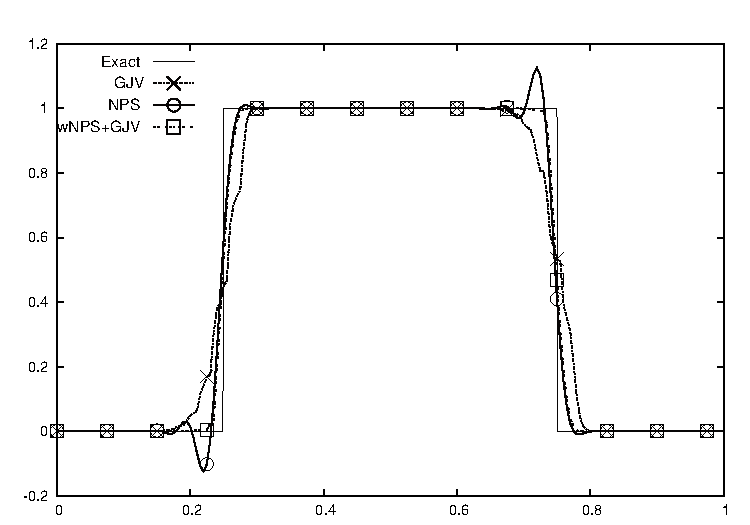
\includegraphics[width=9.65cm]{Figures/paper1/test20_p1_200.pdf}} %
\subfigure[Terracing effect.]{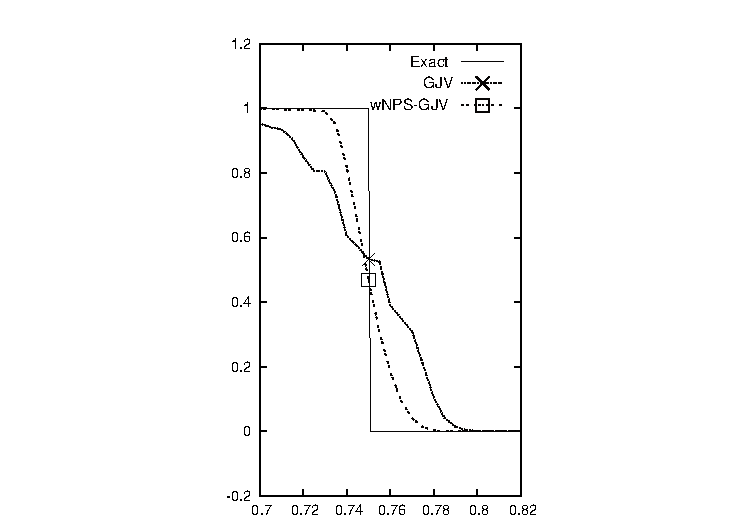
\includegraphics[clip=true, trim=3.8cm 0cm 3.1cm 0cm,width=4.35cm]{Figures/paper1/test20_p1_200_d2.pdf}} %
\caption{Test 1. GJV with $c_{\rm gjv}=0.5$, $q=10$, $p=1$ and $N=200$, Crank-Nicolson, CFL=0.5 and no mass lumping.}\label{fig-pulse1}
\end{figure}

The same test can be used to check the dependence of the DMP property on the variable $c_{\rm gjv}$ in the transport problem.  For this test, we have used the explicit forward Euler method for the integration in time with mass lumping and a CFL of $0.01$ in such a way that the error of the integration in time can be neglected. Fig. \Fig{SZ_AD_2} shows the results obtained when solving problem \Eq{eqtr}-\Eq{trinc} with  wNPS-GJV in Algorithm \ref{alg-wNPS-GJV}. We notice that the larger the value of $q$ the sharper are the oscillations that appear for $c_{\rm gjv} < 0.5$, so we have used $q=100$ to show the results. It is clear that the threshold $c_{\rm gjv} = 0.5$ is sharp; overshoots and undershoots appear in the solution when $c_{\rm gjv}$ is slightly smaller than $0.5$, violating the TVD property.
  %The results obtained using the SC without any linear stabilization are displayed in Fig. \ref{tttPure_AD}. As we expected $\nu = 0.5$ is a threshold for the DMP property. Moreover, in order to avoid the error of the integration in time we have used CFL$=0.01$.
\begin{figure}%
\centering
\subfigure[$c_{\rm gjv}  = 0.49,0.5,0.51$]{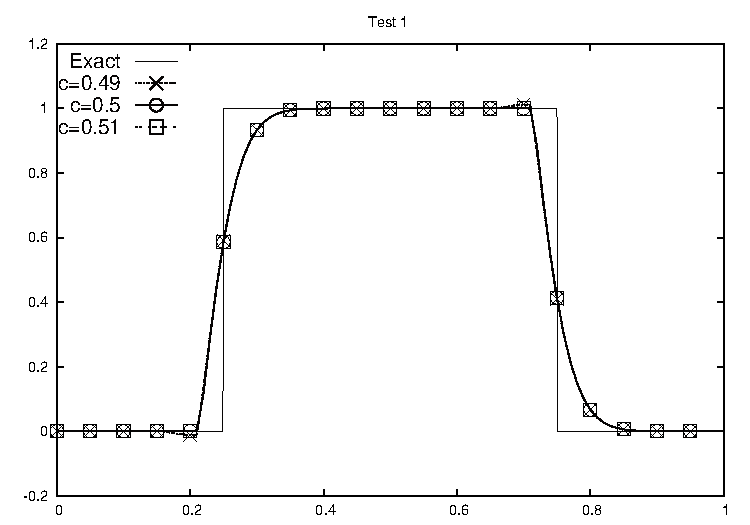
\includegraphics[width=7cm]{Figures/paper1/BurmanSZ.pdf} %
\label{fig-SZ_AD_2_s1} }%
\subfigure[Detail of \subref{fig-SZ_AD_2_s1}]{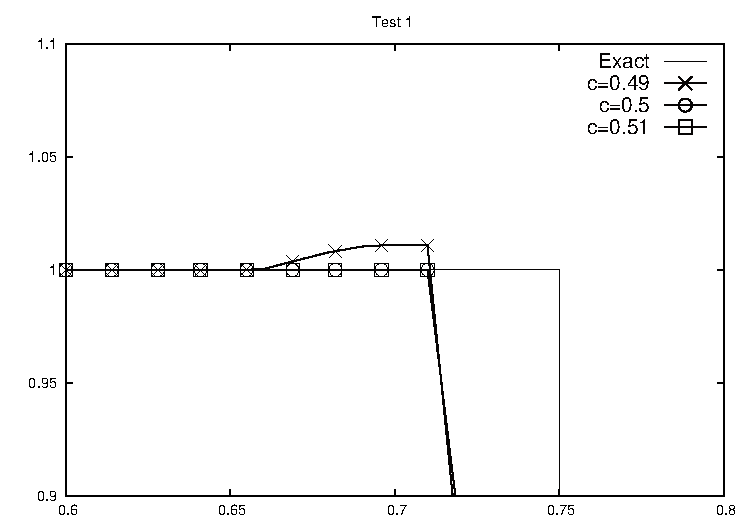
\includegraphics[width=7cm]{Figures/paper1/BurmanSZ1d.pdf}  }%
\caption{Test 1. GJV with $c_{\rm gjv}=0.5$, $q=100$, $p=1$ and $N=100$. Forward Euler with CFL$=0.01$ and mass lumping.}\label{fig-SZ_AD_2}%
\end{figure}


\subsection{Test 2: Convergence to a smooth solution}

In order to check that the order of convergence is not affected by the stabilization added, we will evaluate the error reduction for a sinusoidal when refining the mesh. The test consists in solving the 2$D$ transport equation \Eq{probcont} with $\beta = (1,0)$, $f=0$, initial solution $u_0(x,y) = \sin(2\pi x)$ in $\Omega=[0,1]\times[0,1]$ and periodic boundary conditions in the $x$ direction. The solution presents  maximum and minimum values along two lines ($x=\frac{1}{4}$ and $x=\frac{3}{4}$ respectively for $t=0$) that activate the shock-capturing. The desired behaviour is that this activation does not affect the convergence of the method. The meshes used for the test are regular triangular meshes of size $N_h\times N_h(\times 2)$. The $L^2(\Omega)$ errors are plotted in Fig. \Fig{smooth_sol}. The label $cG$ stands for the continuous Galerkin scheme without any stabilization and is the reference for the desired convergence one wants to attain when solving smooth solutions. It is clear that the convergence order is spoiled when using shock-capturing techniques without any linear stabilization, specially when using the bGJV method. On the other hand the convergence is maintained when both methods are combined with linear stabilization, either wNPS or SUPG. This test provides another motivation to combine linear and nonlinear stabilization, i.e., to have superior convergence in smooth regions.

\begin{figure}
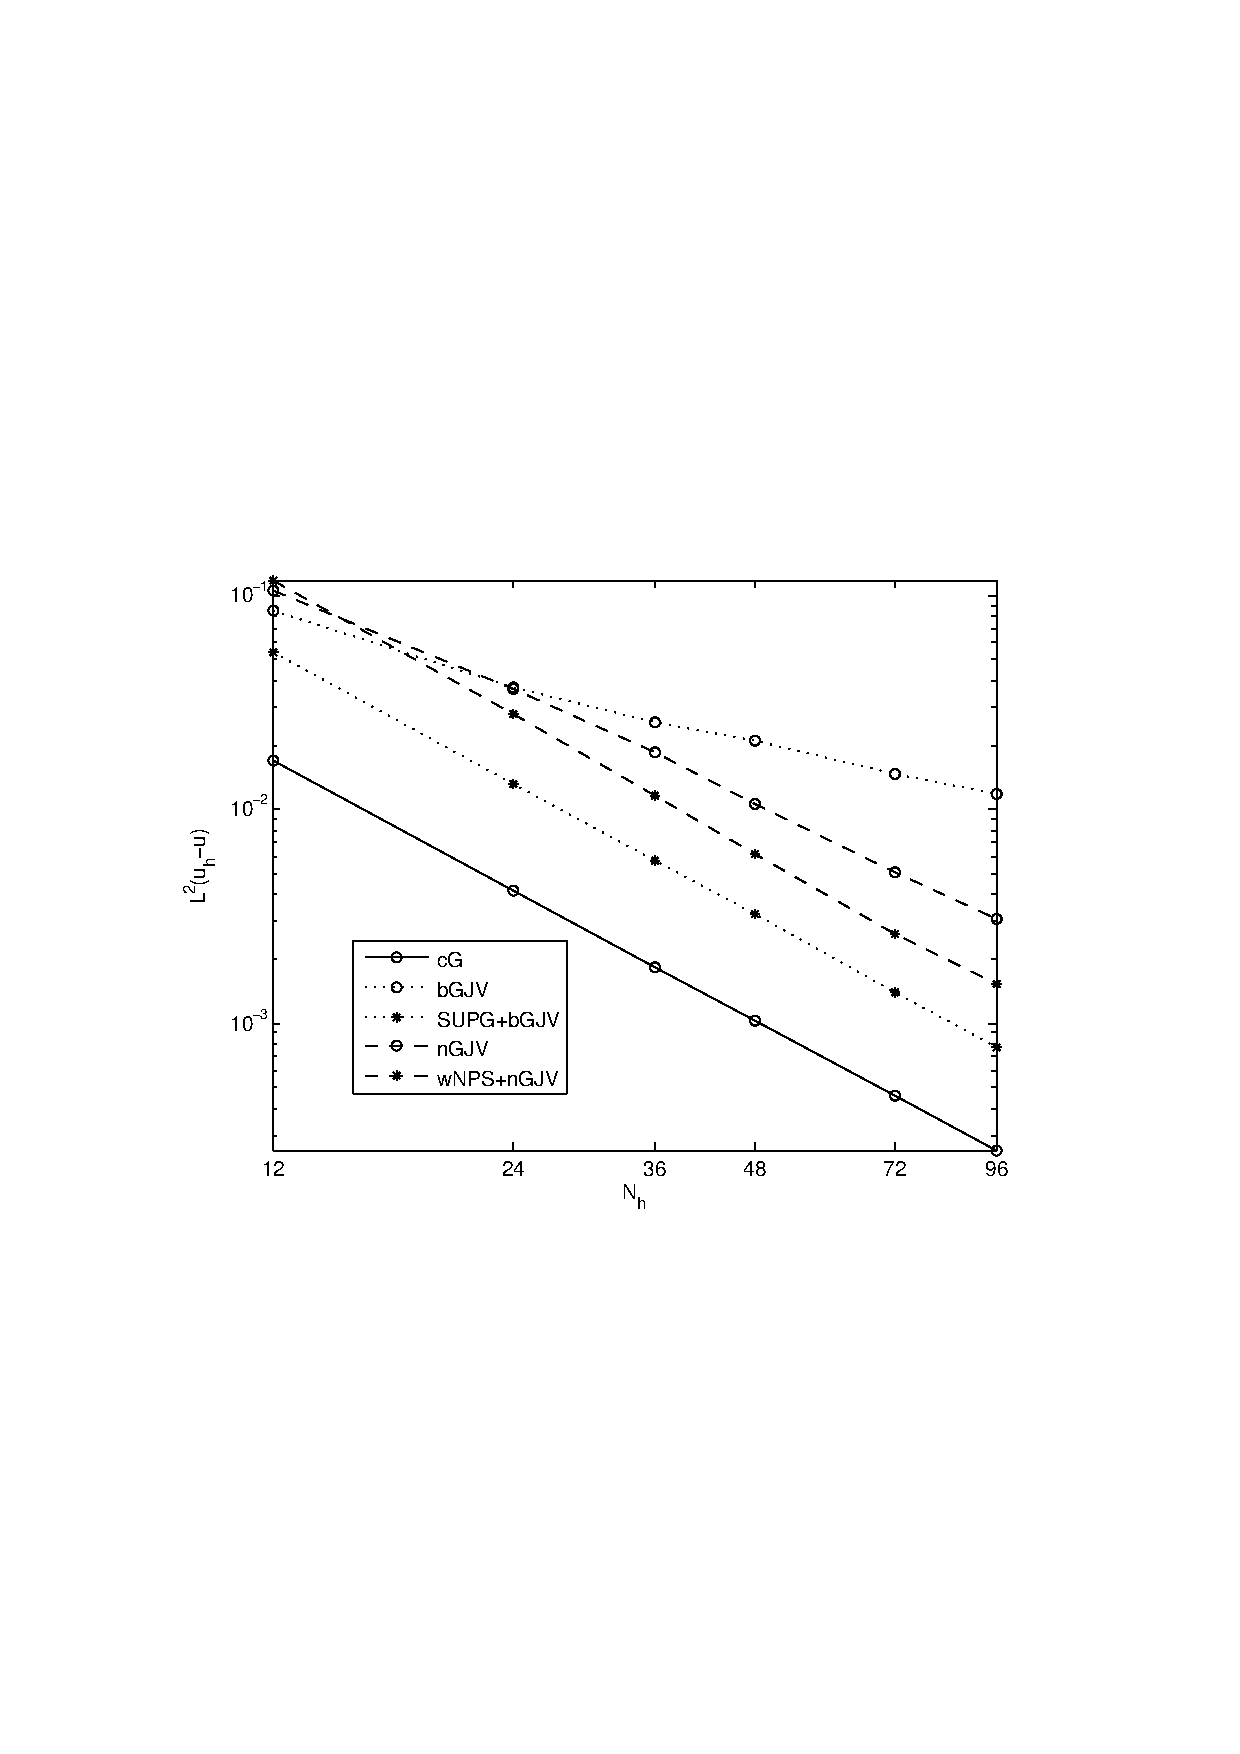
\includegraphics[clip=true, trim=0cm 9cm 0cm 9cm,width=14cm]{Figures/paper1/smooth_conv_test_2D.pdf}%
 \caption{Test 2. $L^2(\Omega)$ error vs size of the mesh. Crank-Nicolson, $t=1$, $\Delta t = 10^{-3}$. No Mass lumping.}\label{fig-smooth_sol}
 \end{figure}

%% \subsection{Test 3: High Order}

%% Eventhough no analysis has been developed, it is interesting to show the performance of the method when high order approximations are used. In order to do so, the test will consist of solving transport equation \Eq{eqtr} in $\Omega = [-1,1]$ with initial condition:
%%  \begin{displaymath}
%%  u_0(x)=\left\{\begin{array}{ll}
%%  \frac{1}{6}\left(G(x,\beta,z-\delta)+G(x,\beta,z+\delta)+4G(x,\beta,z)\right)  & \textrm{if }x\in[-0.8,-0.6]\\
%%  1 & \textrm{if }x\in[-0.4,-0.2]\\
%%  1 - |10(x-0.1)| & \textrm{if }x\in[0,0.2]\\
%%  \frac{1}{6}\left(F(x,\alpha,r-\delta)+G(x,\alpha,r+\delta)+4G(x,\alpha,r)\right) & \textrm{if }x\in[0.4,0.6]\\
%%  0 & \textrm{otherwise},
%%  \end{array}\right.
%%  \end{displaymath} 
%%  with $G(x,\beta,z)=\exp(-\beta(x-z)^2)$, $F(x,\alpha,r)=\sqrt{\max(1-\alpha^2(x-r)^2,0)}$, $r=0.5$, $z=-0.7$, $\delta=0.005$, $\alpha=10$, $\beta=\displaystyle\frac{\log 2}{36\delta^2}$. The solution is computed at time $T=2$ after one exact period. The solution consists of a smooth but narrow Gaussian, a square pulse, a sharp triangle and a combination of half-ellipses. The test includes various features that we want our methods to capture; its solution is a combination of a continuous but not differentiable linear function (which is badly approximated if the function is overdiffusive), a discontinuous shock and continuous but sharp functions (which should be better captured with $p$ refinement of the mesh).
 
%% To check the behaviour of the method, results are obtained with different order but maintaining the degrees of freedom of the problem, so the  following pairs of parameters have been used: $(p,N) = (1,800), (2,400), (4,200), (8,50)$. We solved the problem using Crank-Nicolson and a CFL coefficient of $0.5$. Moreover the parameters $\nu$ and $q$ have been empirically optimazed to be $\nu = (8p-6)^{-1}$ and $q=10$. The results obtained with the Scott-Zhang stabilization are plotted in Fig. \Fig{high_order_1D}. The accuracy of the method is mantained when increasing the order of approximation but it is clear that the shocks are better captured when the mesh is finer.

%%  \begin{figure}
%%  \includegraphics[width=16cm]{Figures/paper1/highorder1D.pdf} %
%%  \caption{Test 3. AD + NPS stabilization (\Eq{SZstab}-\Eq{stproj1}-\Eq{projSZ}-\Eq{tildeltaSZ} formulation). $(p,N) = (1,800), (2,400), (4,200), (8,100)$. Crank-Nicolson with CFL=0.5. NO Mass lumping.}\label{fig-high_order_1D}
%%  \end{figure}

\subsection{Test 3: Multidimensional transport problem} 
Now, we want to show the performance of nGJV and bGJV nonlinear stabilization for multidimensional problems. We solve the $2D$ transport equation \Eq{eqtr} in $\Omega = [0,1]\times[0,1]$ with $\bb=(-2\pi (y-0.5), 2\pi (x-0.5))$. The initial solution is given in \cite{dmitri_kuzmin_guide_2010} and its interpolation in a mesh of $250\times250$ bilinear elements is displayed in Fig. \Fig{kuzmin0}. %We have extended the definition of the amount of artificial viscosity as it is shown in \Eq{gjvisc}. 
 

\begin{figure}%
\centering
\subfigure[Nodally exact initial solution and error regions.]{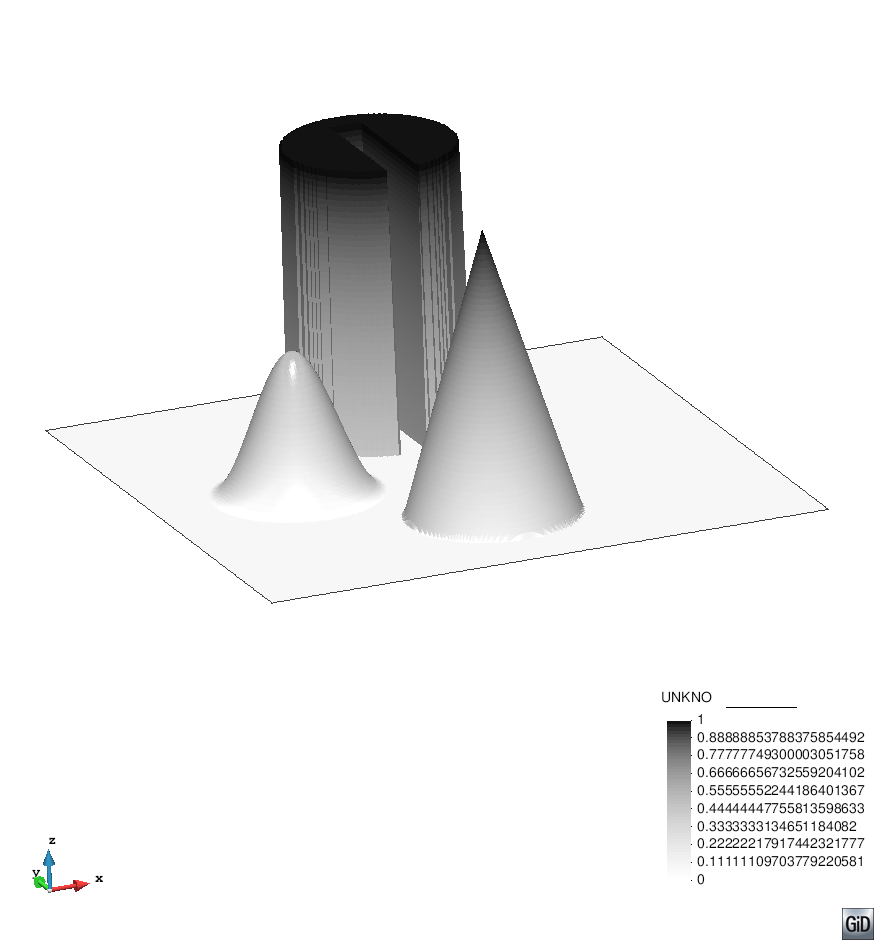
\includegraphics[clip=true, trim=1.6cm 11cm 1.6cm 3cm,width=7.9cm]{Figures/paper1/inisol.png}\label{fig-kuzmin0}}%
\subfigure[Error regions]{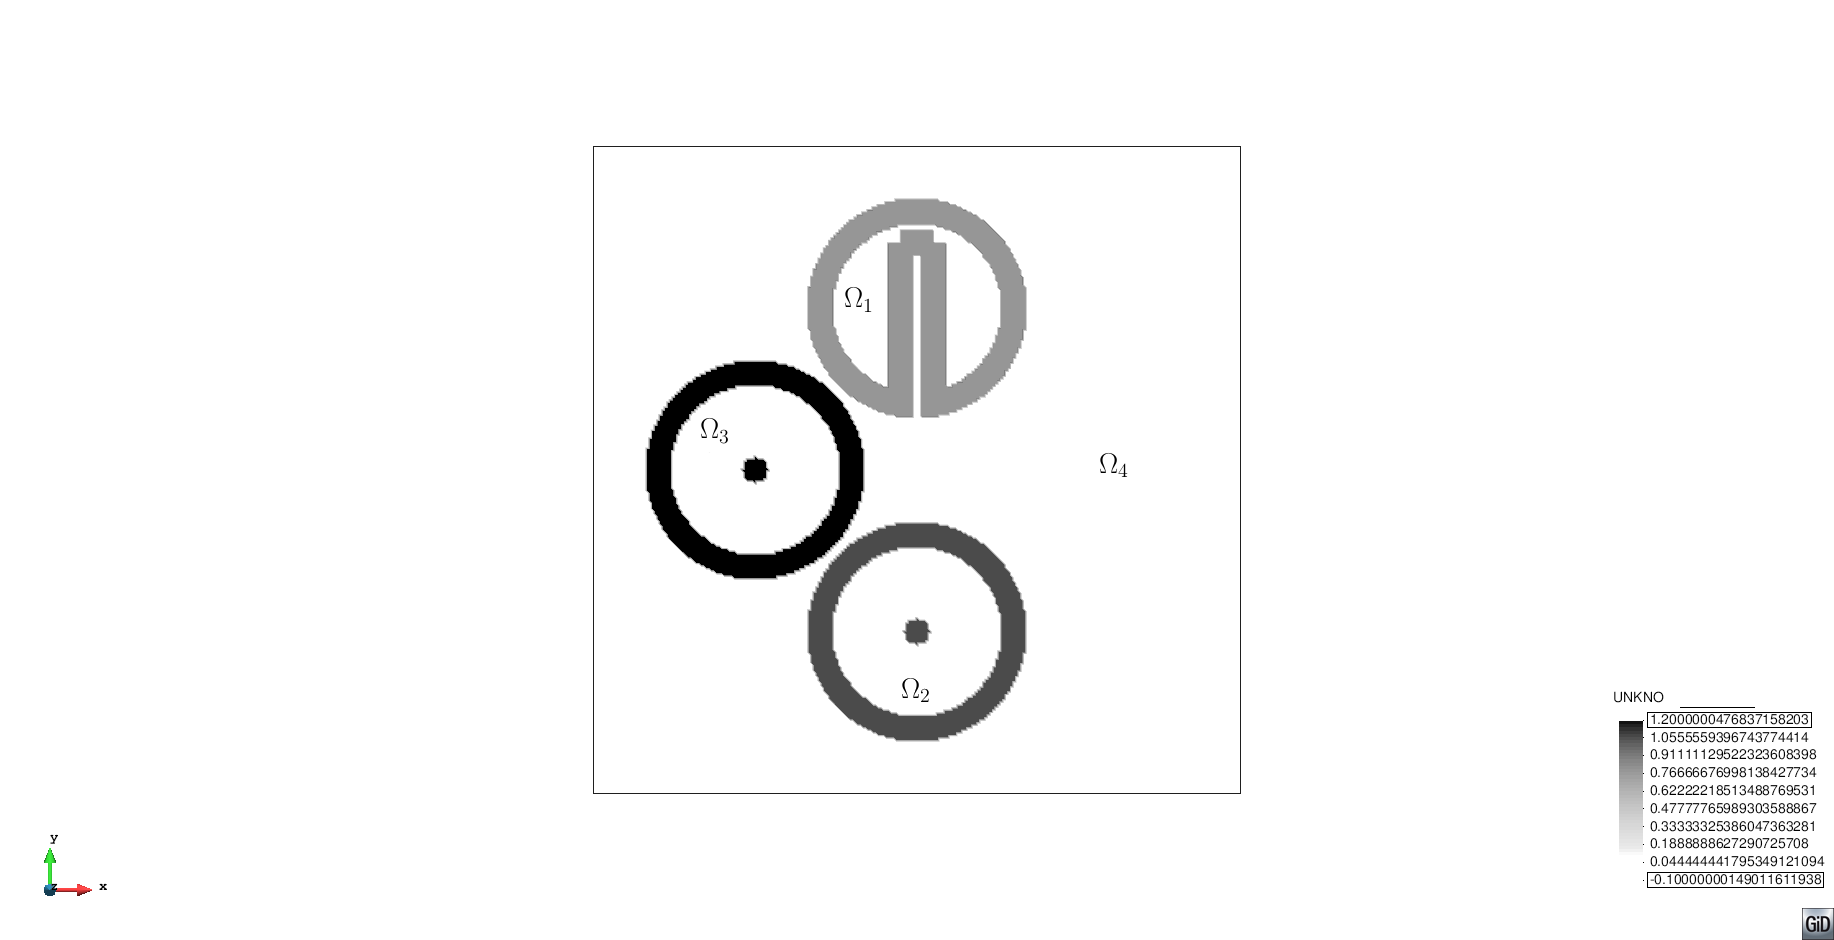
\includegraphics[clip=true, trim=15cm 4cm 15cm 4cm,width=7.9cm]{Figures/paper1/error_regions.png}\label{fig-err_reg}}
%{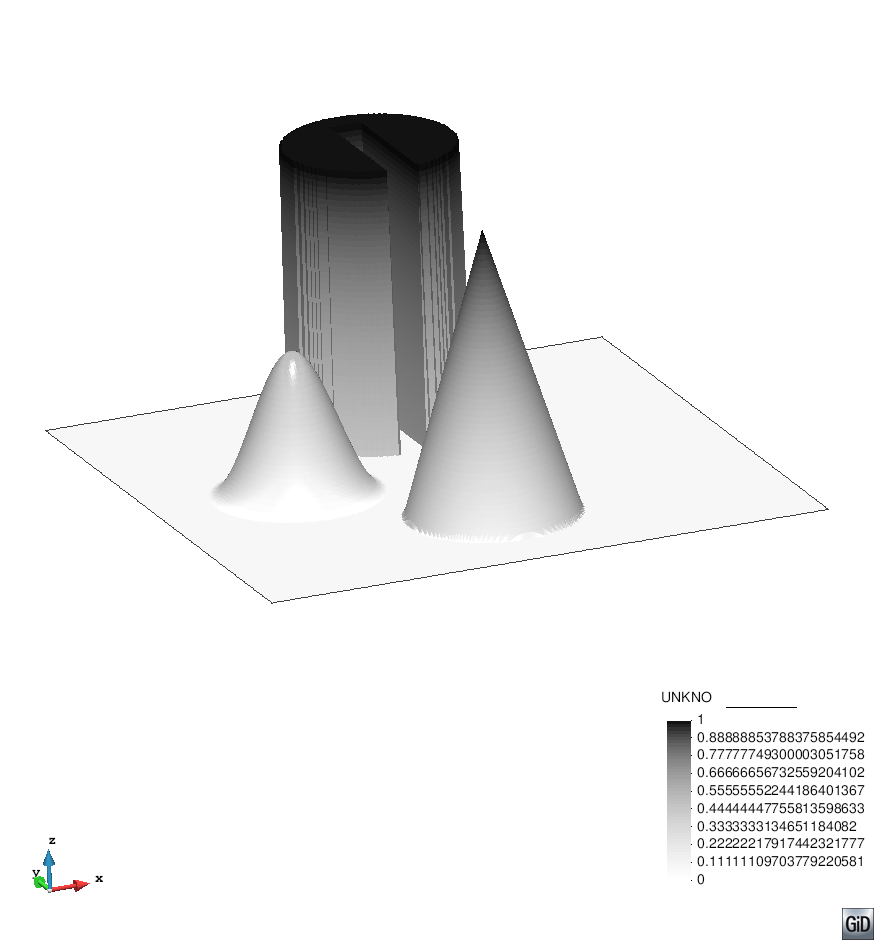
\includegraphics[clip=true, trim=25.5cm 1.1cm 0.9cm 23.1cm, width=2cm]{Figures/paper1/inisol.png}}%
%{\includegaphics[clip=true, trim=25.5cm 1.1cm 0.9cm 23.1cm, width=2cm]{Figures/paper1/15_SUPG_GJV_250_notunning.png}}%
\caption{Test 3. Nodally exact initial solution}\label{fig-algo}
\end{figure}


The solution is computed until $t=1$ with a $250 \times 250 (\times 2)$ triangular mesh. Crank-Nicolson with time step $\Delta t = 2\cdot 10^{-4}$ and without mass lumping is used for the integration in time.  We compare the performance of nGJV and bGJV (with and without linear stabilization), EV, and RV  methods. The value of the constant of each method is specified in Algorithm \ref{alg-wNPS-GJV} and all of them have been optimized to obtain the best results. With regard to the EV formulation, we have considered the value of the constants following \cite{guermond_entropy_2011}.\footnote{Let us note that the results for the EV method have been obtained with the entropy function $\eta = (u- 1/2)^2$. This choice is basic to reproduce these results, since the discontinuities under consideration have plateaus on $u = 0$ and 1, and the use of $\eta = u^2$ or $\eta = (u-1)^2$ leads to worse results.} %The optimal definition of the entropy function to be used in the EV method seems to be a problem-dependent task. %How to properly define the optimal entropy function in more complex situations is unclear.
An approximation of the $L^2$ error after one cycle has been computed in $4$ different regions $\Omega_1$, $\Omega_2$, $\Omega_3$, $\Omega_4$ that are plotted in Fig. \Fig{err_reg}. The first $3$ regions consist of a layer of width $2\cdot 10^{-2}$ around the regions where the function or its gradient change abruptly. The results are collected in Table \ref{tab-ex15_malla2D_new}. Most of the error is concentrated in $\Omega_1$, the layer around the cylinder. In general all the methods give a similar order of error in each region and there is no method that clearly outstands from the rest. 
%The nGJV shock capturing is the one with less error on the cylinder layer, while RV and EV are the best in $\Omega_2$ and $\Omega_3$ respectivley. In $\Omega_4$, both RV and nGJV are very close. 
However, the numerical results obtained with the different methods are certainly different, as one can observe in the actual results plotted in Fig. \Fig{triangle1} at $t = 1$. The solutions obtained with nGJV are oscillation-free up to solver tolerance error. Even though the nGJV method without stabilization gives the smallest error in $\Omega_1$, the terracing effect can be appreciated around the cylinder. When wNPS stabilization is added, the solution is smoothed in the region. The strongest oscillations are observed in the SUPG-RV solution. The EV solution presents oscillations on the $u_h=0$ plateau around the shapes that cannot be clearly observed in the plot, and these oscillations become larger when the problem is solved with a quadrilateral mesh. % We note that the entropy function has been optimized to adequate to a function with plateaus at $0$ and $1$. E.g., if $\eta=u_h^2$ instead of $(u_h - 0.5)^2$, the results present strong wiggles on the regions where $u=0$.
\begin{table}
\centering
\begin{tabular}{lccccc}
\hline
Method &  $\Omega_1$ &  $\Omega_2$ &  $\Omega_3$ &  $\Omega_4$\\\hline
wNPS + bGJV  &  2.961e-01 & 1.338e-02
&  3.071e-03
&  1.033e-02\\

SUPG + bGJV  &
  2.698e-01    
  & 1.234e-02
  & 2.303e-03
  & 8.929e-03 \\
    None + EV  &
  2.854e-01     
&  9.123e-03
&  8.412e-04
&  1.287e-02\\

SUPG + RV  &
  2.634E-01     
&  7.551e-03
&  2.063e-03
&  6.933e-03 \\
nGJV  &
  2.318e-01     
&  1.015e-02
&  1.914e-03
&  6.957e-03\\

wNPS + nGJV  &
  2.848e-01     
&  1.119e-02
&  1.546e-03
&  7.834e-03\\
\hline
\end{tabular}
\caption{Test 3. $\|u-u_h\|_{\Omega_i}$}\label{tab-ex15_malla2D_new}
\end{table}
\begin{figure}%
\centering
\subfigure[{ wNPS-bGJV}]{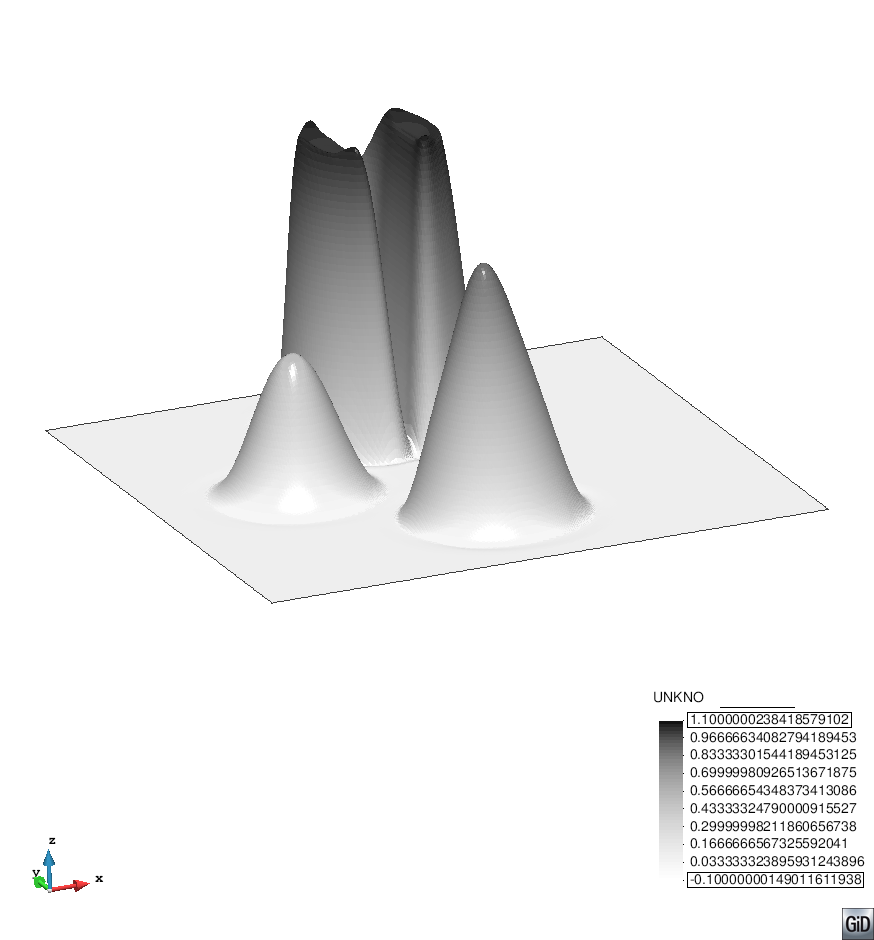
\includegraphics[clip=true, trim=1.6cm 11cm 1.6cm 3cm,width=7.9cm]{Figures/paper1/15_SZ_GJV_T.png}}%
%\subfigure{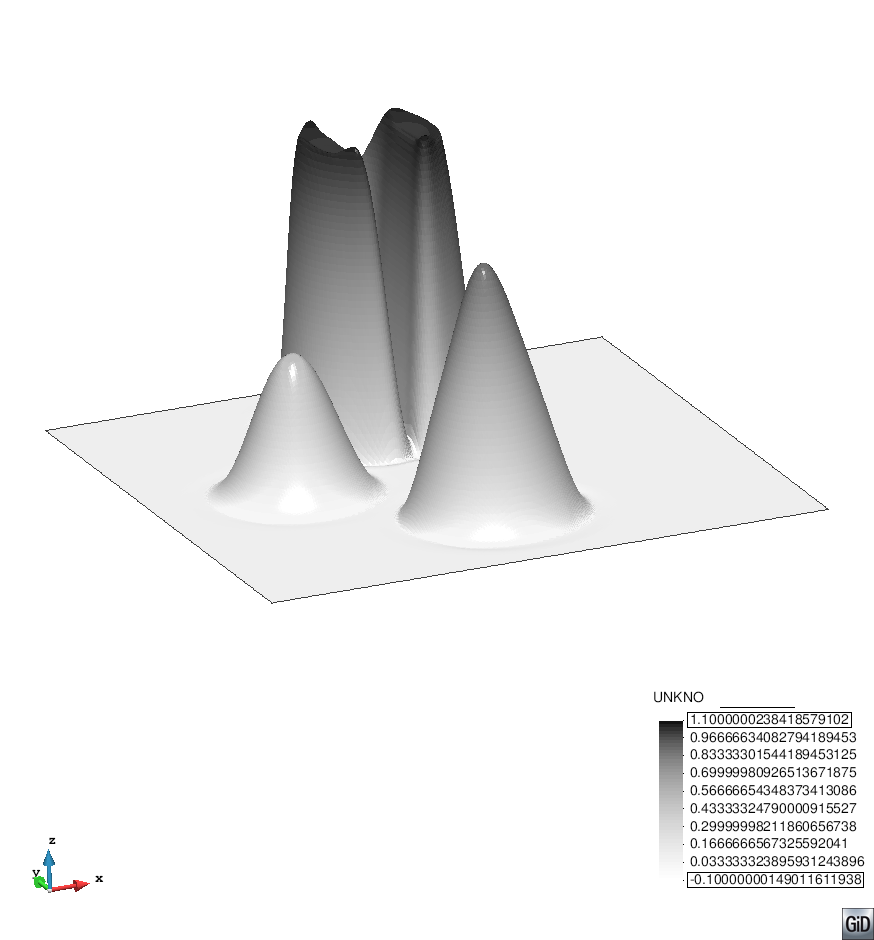
\includegraphics[clip=true, trim=15.5cm 1.1cm 0.9cm 11.65cm, width=1.75cm]{Figures/paper1/15_SZ_GJV_T.png}}%
\subfigure[{SUPG-bGJV}]{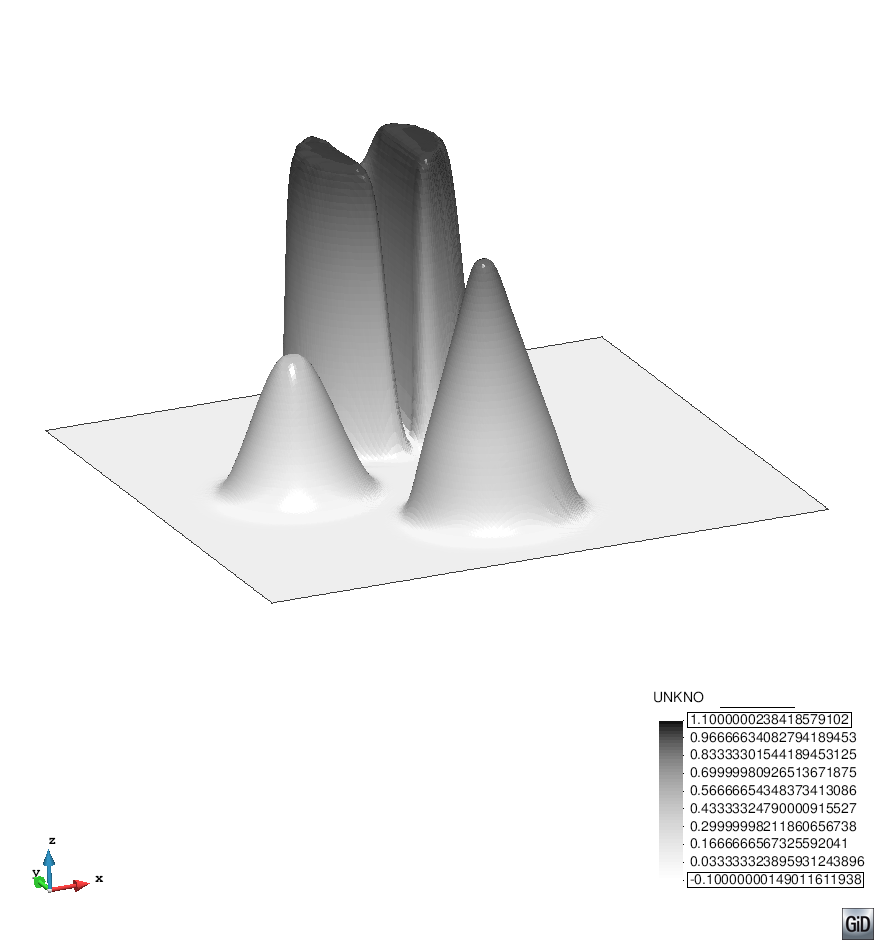
\includegraphics[clip=true, trim=1.6cm 11cm 1.6cm 3cm,width=7.9cm]{Figures/paper1/15_SUPG_GJV_T.png}\label{fig-sq1-supgbgjv}}\\%
%\subfigure{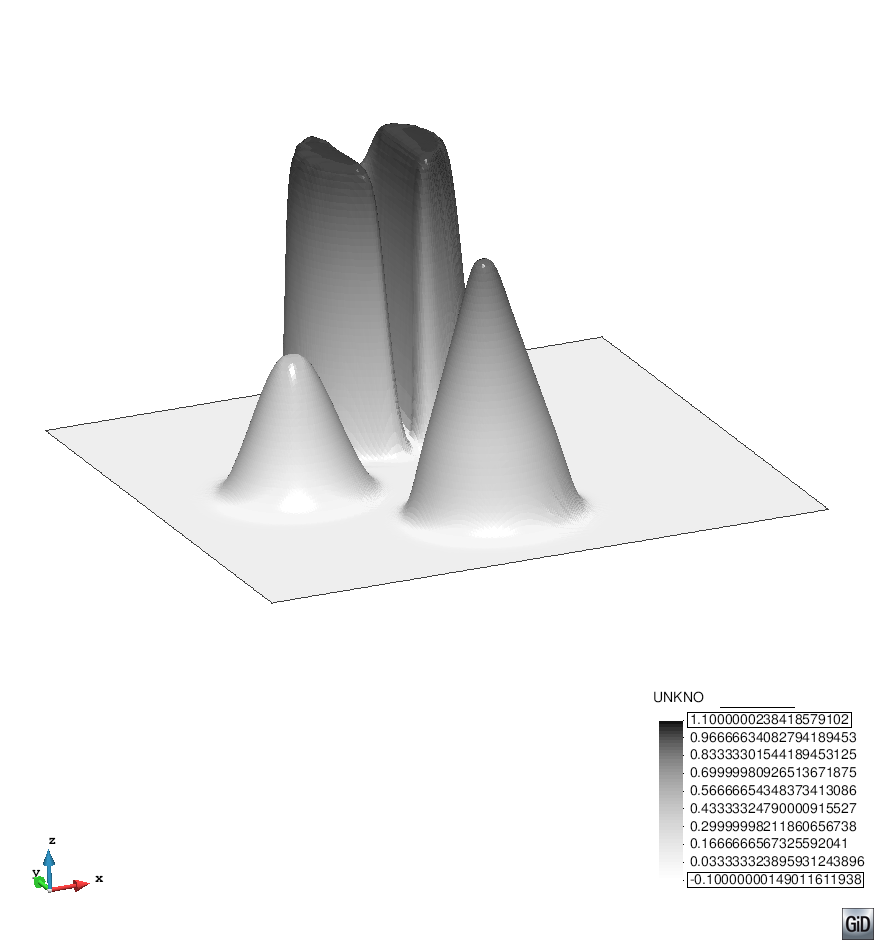
\includegraphics[clip=true, trim=15.5cm 1.1cm 0.9cm 11.65cm, width=1.75cm]{Figures/paper1/15_SUPG_GJV_T.png}}
\subfigure[{EV}]{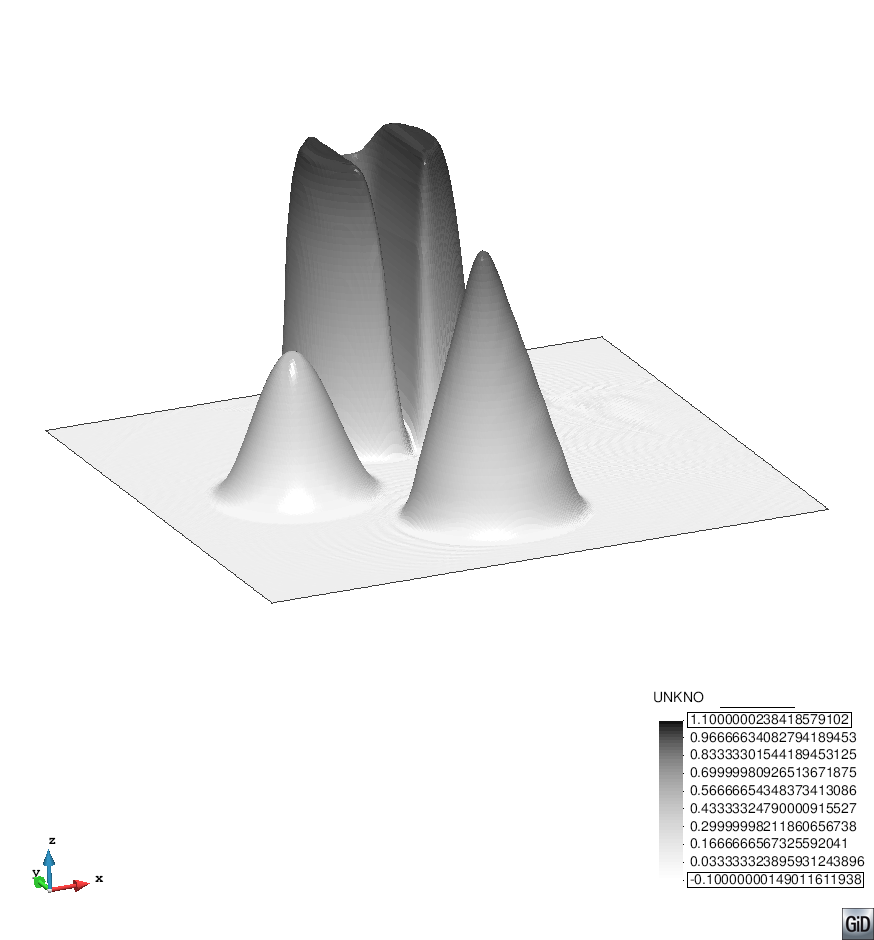
\includegraphics[clip=true, trim=1.6cm 11cm 1.6cm 3cm,width=7.9cm]{Figures/paper1/15_None_EV_T.png}}%
%\subfigure{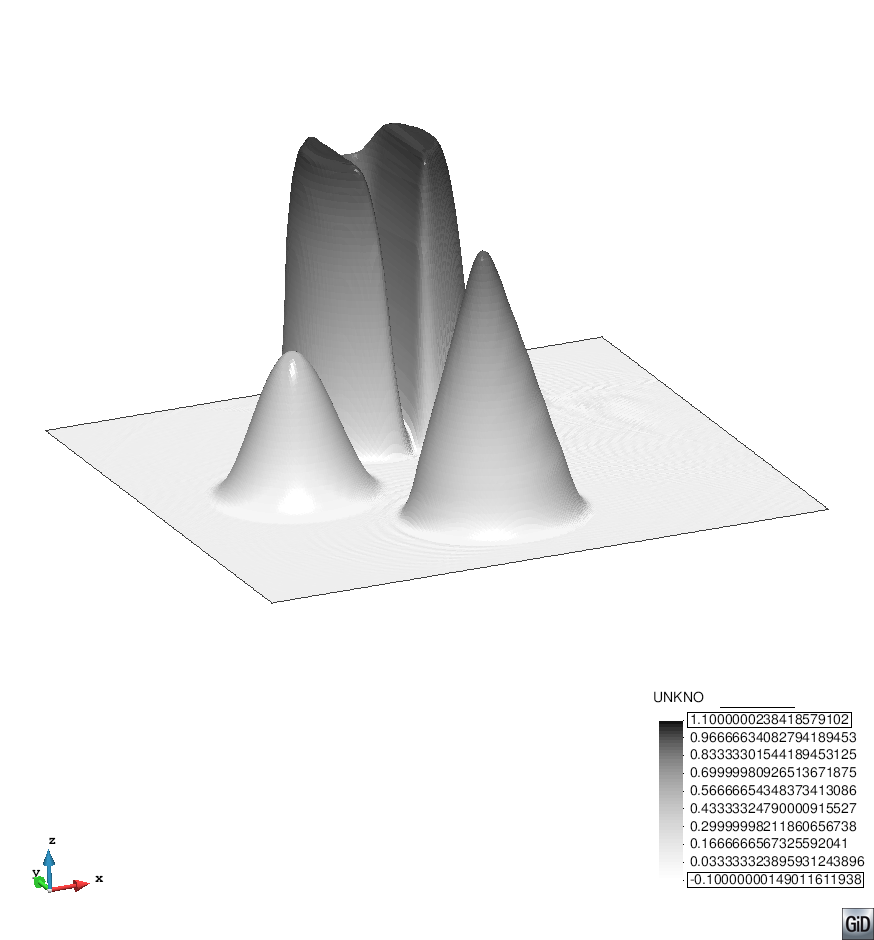
\includegraphics[clip=true, trim=15.5cm 1.1cm 0.9cm 11.65cm, width=1.75cm]{Figures/paper1/15_None_EV_T.png}}\\ %
\subfigure[{SUPG-RV}]{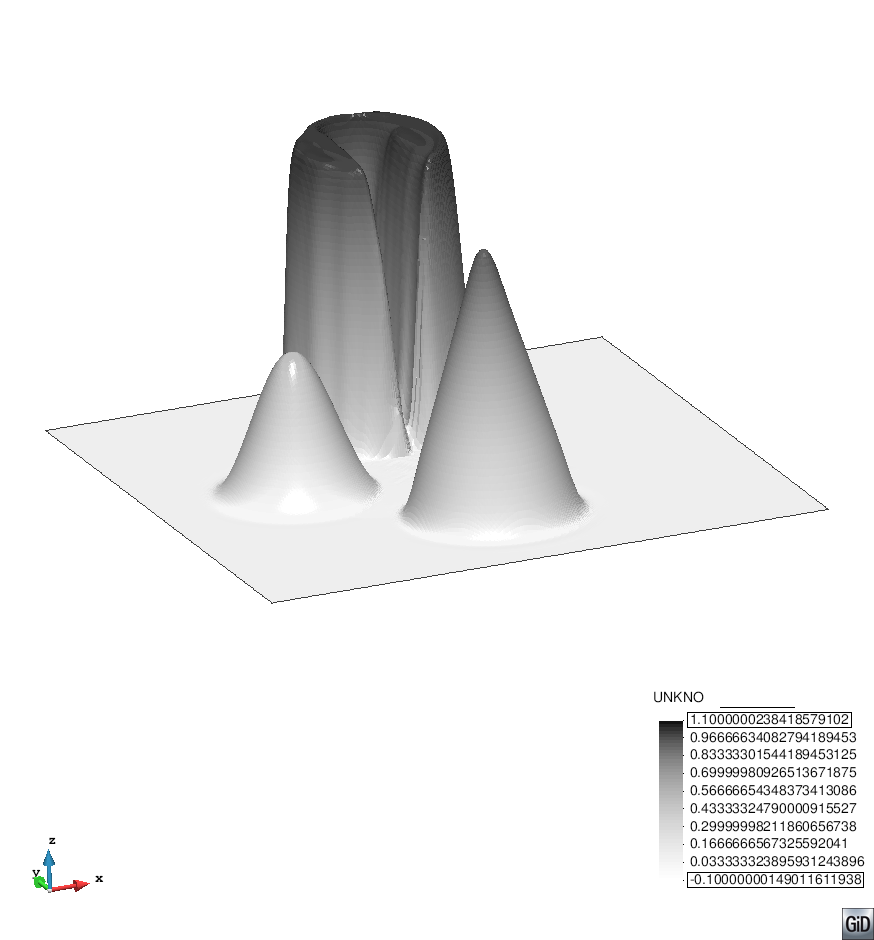
\includegraphics[clip=true, trim=1.6cm 11cm 1.6cm 3cm,width=7.9cm]{Figures/paper1/15_SUPG_RV_T.png}}\\%
%\subfigure{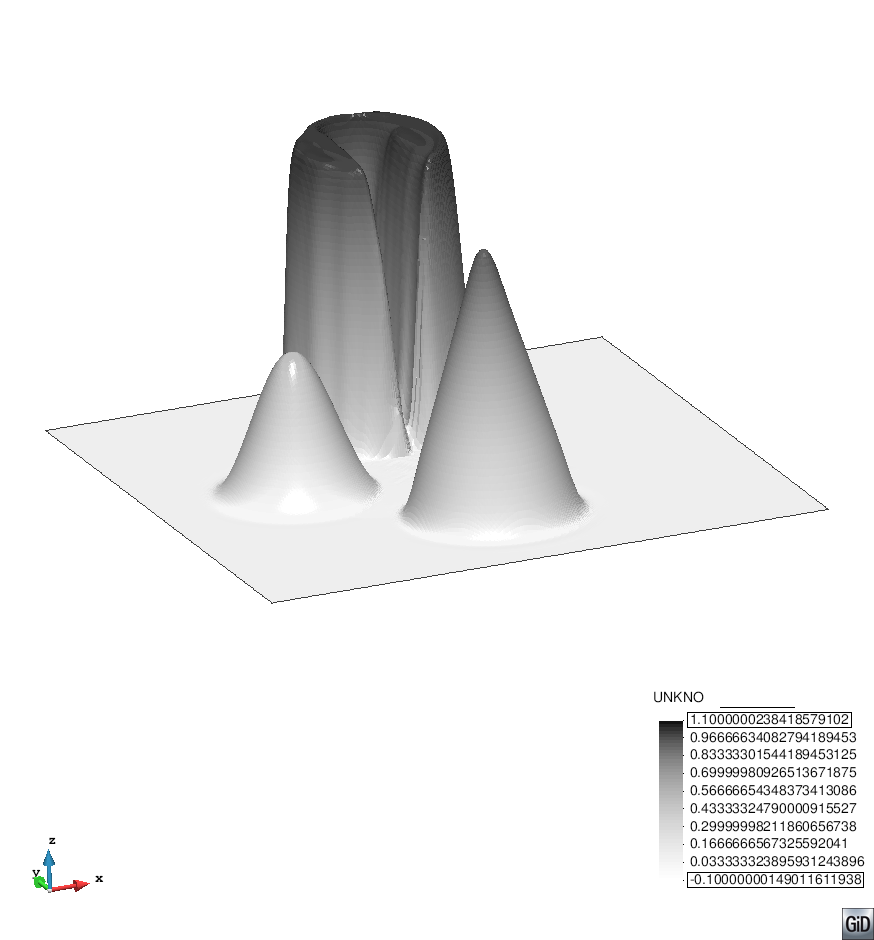
\includegraphics[clip=true, trim=15.5cm 1.1cm 0.9cm 11.65cm, width=1.75cm]{Figures/paper1/15_SUPG_RV_T.png}}\\%
\subfigure[{nGJV}]{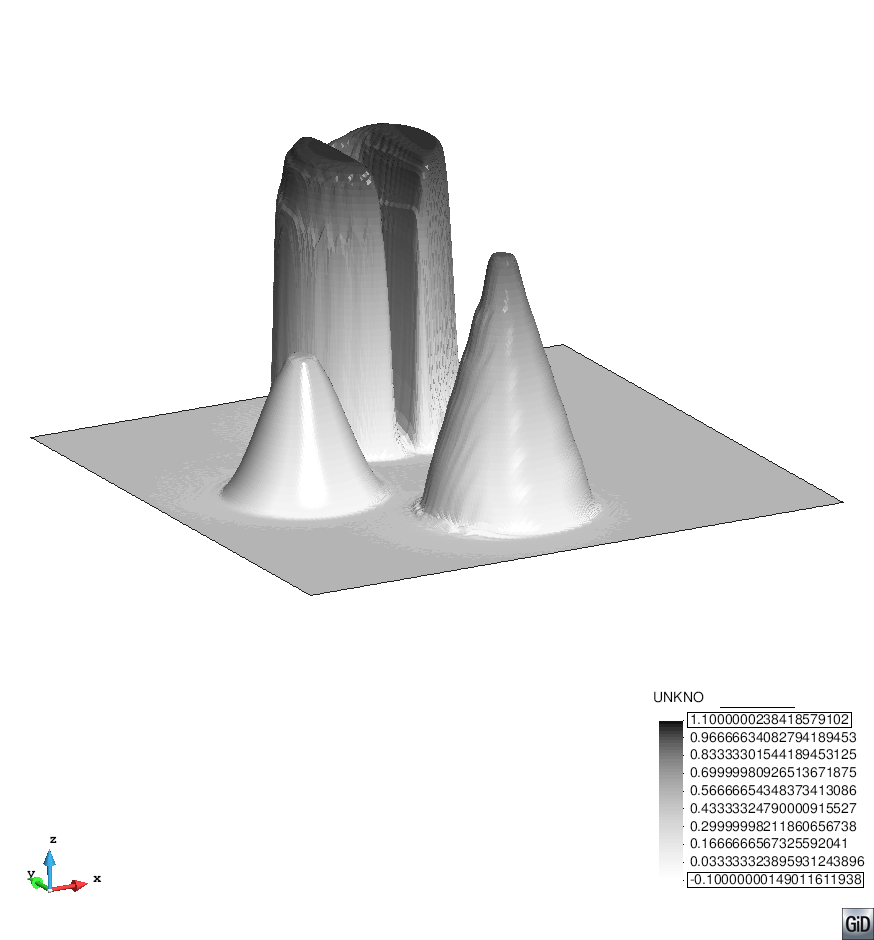
\includegraphics[clip=true, trim=1.6cm 11cm 1.6cm 3cm,width=7.9cm]{Figures/paper1/15_None_PGJV_T.png}}%
%\subfigure{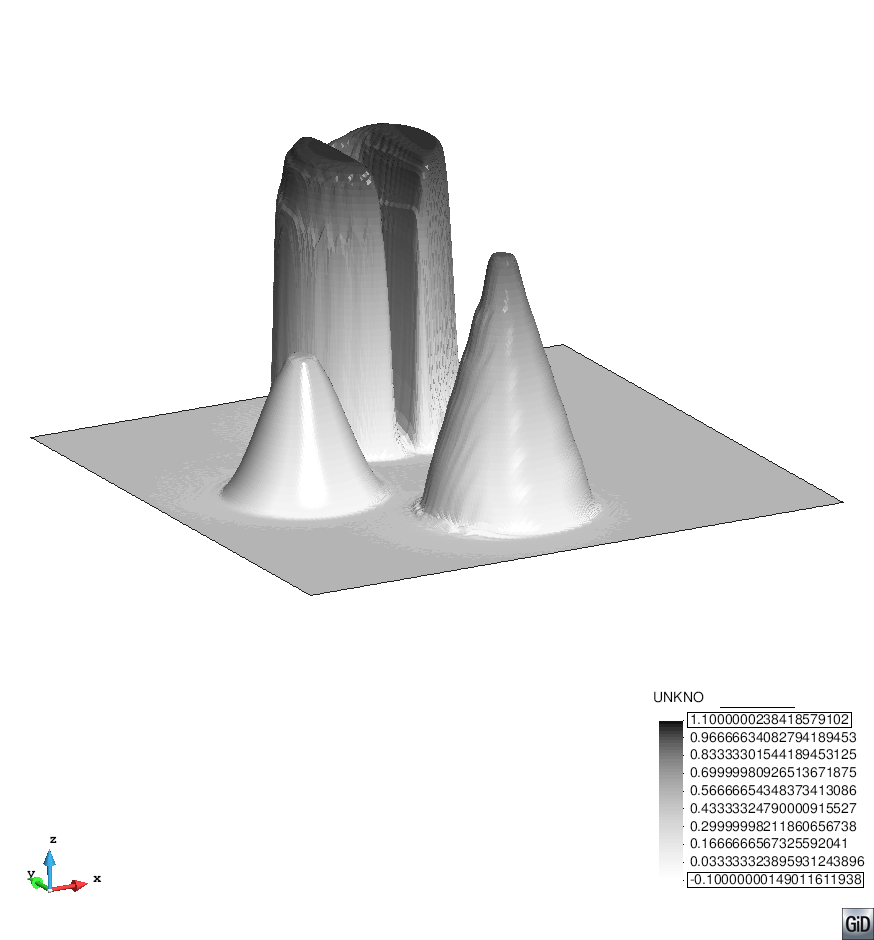
\includegraphics[clip=true, trim=15.5cm 1.1cm 0.9cm 11.65cm, width=1.75cm]{Figures/paper1/15_None_PGJV_T.png}}\\%
\subfigure[{ wNPS-nGJV}]{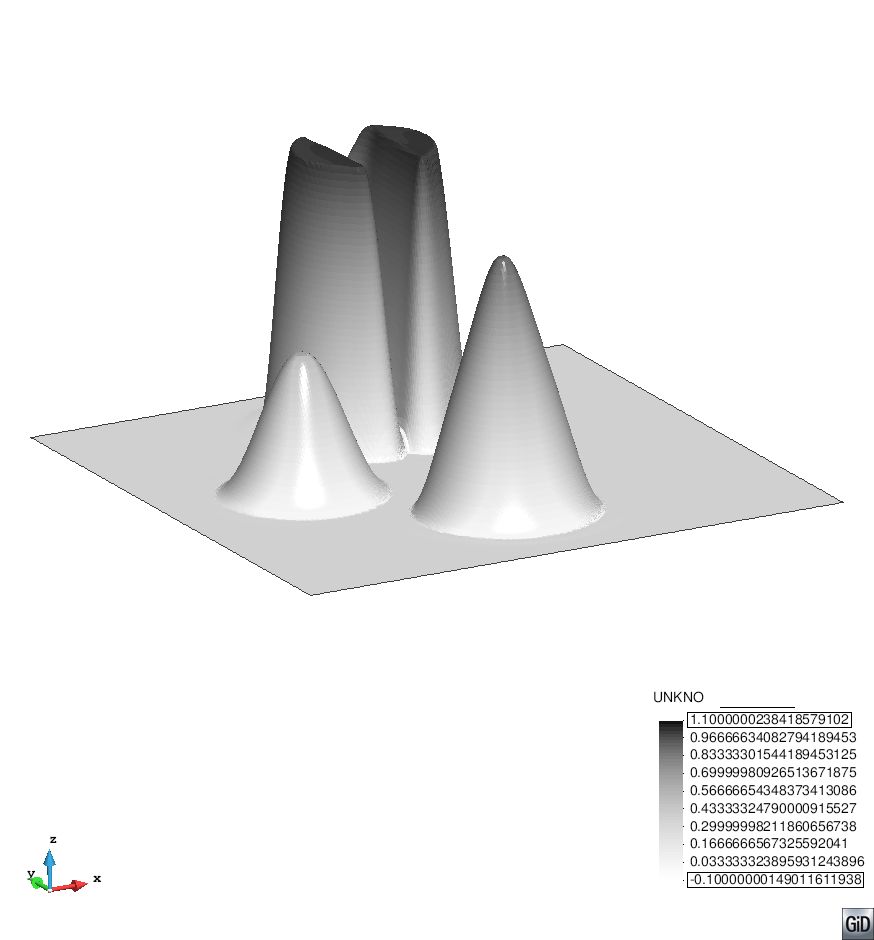
\includegraphics[clip=true, trim=1.6cm 11cm 1.6cm 3cm,width=7.9cm]{Figures/paper1/15_SZ_PGJV_T.png}}%
%\subfigure{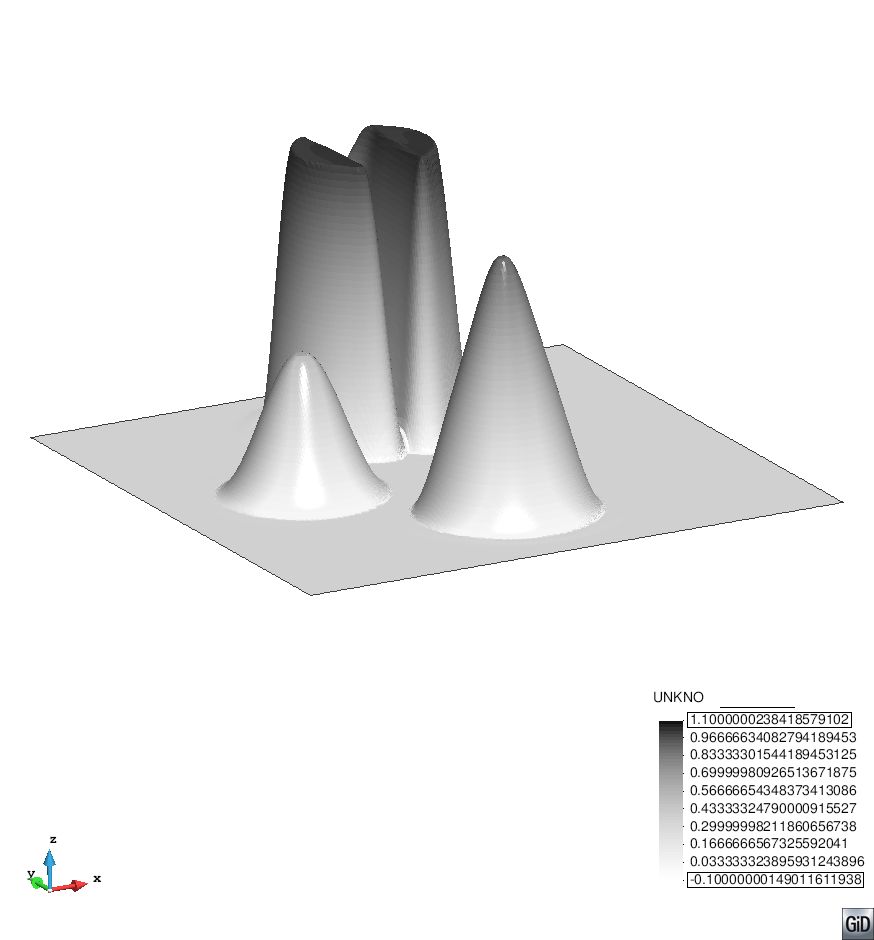
\includegraphics[clip=true, trim=15.5cm 1.1cm 0.9cm 11.65cm, width=1.75cm]{Figures/paper1/15_SZ_PGJV_T.png}}
\caption{ Test 3. Results at $t = 1.0$. Space discretization with $p=1$ and $250\times 250 (\times 2)$ triangular mesh. Time discretization with Crank-Nicolson, $\Delta t = 2 \cdot 10^{-4}$ and without mass lumping. Results for different schemes at $t = 1 $.}\label{fig-triangle1}
\end{figure}


%Since Next, we apply the nGJV method in a non strictly acute mesh and no mass lumping, with the constant $c_{\rm gjv} = \frac{1}{(d+1) \sigma_K \sin(\pi / 6)}$

The results reported in Fig. \Fig{triangle1} are at the final stage of the computation, i.e., $t=1$, and the oscillations have already been smoothed out. In order to better evaluate how the different methods succeed eliminating oscillations, we introduce the oscillation function
%In order to show the behaviour at the first steps one can compute the value%It comes from the fact that some methods suffer at the first time steps, untill diffusion has smoothed sharp discontinuities out. Further, we report in Table \ref{tab-triangle} the oscillations, i.e. 
\begin{align*}
&{\rm osc}(t) = \max_{(x,y)\in \Omega} \left\{0 , u_h(x,y,t) - 1 , -u_h(x,y,t) \right\}.
\end{align*}
We compute the mean value of the parameter ${\rm osc(t)}$ in bunches of $50$ time steps and the time evolution of this quantity for the different methods is plotted in Fig \Fig{osc}. It can be appreciated that the method with the smallest overshoots and undershoots is nGJV without any linear stabilization; when the wNPS is added, the order of the oscillations is still very low. We remark that the DMP is not exactly attained for the nGJV method since we are considering non-acute meshes, no mass lumping, and inexact time integration. bGJV shows smaller oscillations when combined with SUPG stabilization than with the wNPS; it is noticeable the good behavior of bGJV with SUPG compared to the traditional RV-SUPG approach. Focusing on the first time steps, where the stronger oscillations occur, RV and bGJV present strong violations of the DMP (either wiht SUPG and with wNPS linear stabilization). These oscillations remain for SUPG-RV and wNPS-bGJV methods during the whole computation. This oscillatory behaviour is clearly observed  in Fig. \Fig{osrv}, where we plot the solutions obtained  at time $t=0.01$. 

\begin{figure}%
\centering
\subfigure[${\rm osc(t)}$ in time]{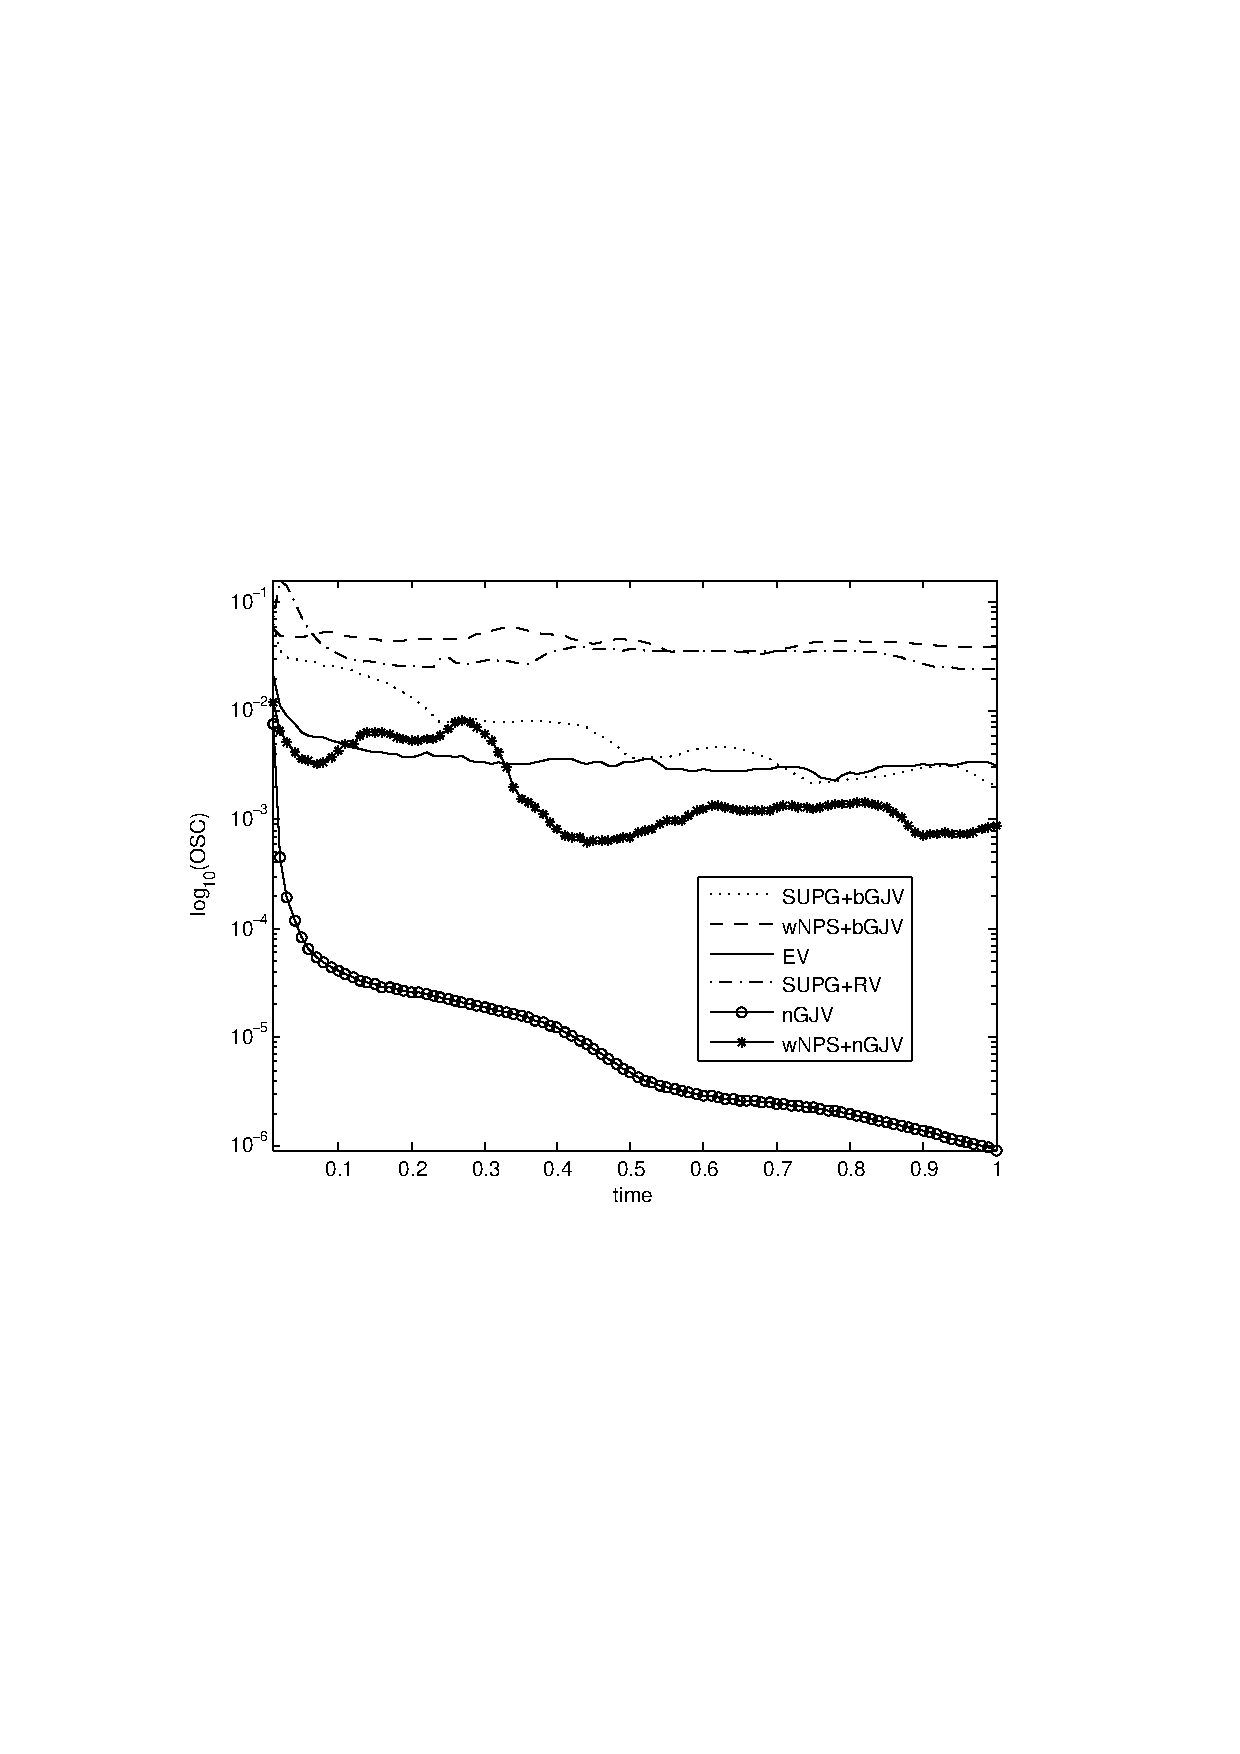
\includegraphics[clip=true,  trim=3cm 9cm 4cm 9cm,width=7.9cm]{Figures/paper1/osc_time_tr.pdf}\label{fig-osc}}%
%\subfigure[${\rm osc(t)}$ in time]{\includegraphics[clip=true,  trim=3cm 9cm 4cm 9cm,width=7.9cm]{Figures/paper1/osc_time_tr_new.pdf}}%
\subfigure[{SUPG-RV, $t = 0.01 $}]{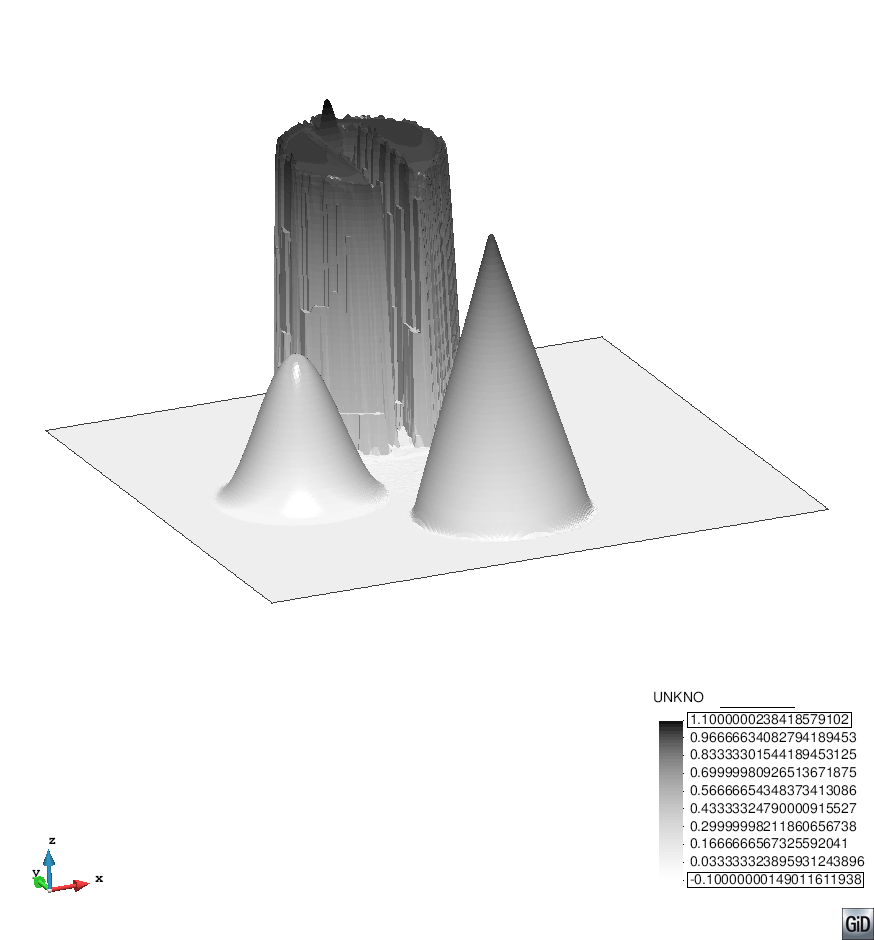
\includegraphics[clip=true, trim=1.6cm 11cm 1.6cm 3cm,width=7.9cm]{Figures/paper1/15_SUPG_RV_T_001.png}\label{fig-osrv}}\\%
\caption{Test 3. Evolution of the parameter ${\rm osc}$. Detail of the solution for the SUPG-RV at $t=0.01$. Space discretization with $p=1$ and $250\times 250 \times 2$ triangular mesh. Crank-Nicolson, $\Delta t = 2 \cdot 10^{-4}$ and no mass lumping.}\label{fig-osctime}
\end{figure}

%Out of these results, we can draw some conclusions. In the first stages of the computation, i.e. the results for $t = 10^{-2} \, {\rm s}$ in Figs. \Fig{square001}-\Fig{triangle001} and Table \ref{tab-triangle}, we observe that traditional SUPG-RV methods exhibit the strongest oscillations. The bGJV shock-capturing technique, both with SUPG and  wNPS stabilization, presents similar oscillations on the triangular mesh. However, on the quadrilateral mesh, SUPG-bGJV leads to excellent results whereas  wNPS-bGJV is over-dissipative. It is clear out of these results, that EV and nGJV (alone or with  wNPS stabilization) are the best methods for this case. It is remarkable the value of the largest oscillation of the nGJV method in both meshes and the  wNPS-nGJV method in the quadrilateral mesh. We remark that the DMP cannot be exactly attained since we are considering non-acute meshes, no mass lumping and inexact time integration.

%TRIANGULAR MESH  
%\begin{table}
%\centering
%\begin{tabular}{ccccc}
%\hline
%Method  & Mesh type & $\max {\rm osc}(\cdot)$ & ${\rm osc}(0.01)$ & ${\rm osc}(1.0)$ \\\hline
%
% wNPS-bGJV & triangles    &  1.173e-01 &  7.304e-02 &  6.071e-02 \\
%             & quads        &  6.300e-02 &  5.908e-02 &  3.990e-03 \\\hline
%SUPG-bGJV    & triangles    &  2.200e-01 &  3.793e-02 &  1.758e-03 \\
%             & quads        &  1.432e-01 &  2.044e-02 &  3.987e-03 \\\hline
%EV           & triangles    &  6.739e-02 &  1.290e-02 &  2.310e-02 \\
%             & quads        &  4.911e-02 &  9.113e-03 &  2.604e-02 \\\hline
%SUPG-RV      & triangles    &  1.727e-01 &  1.190e-01 &  2.560e-02 \\
%             & quads        &  2.143e-01 &  1.831e-01 &  2.962e-02 \\\hline
%nGJV         & triangles    &  5.449e-02 &  7.637e-04 &  1.816e-07 \\
%             & quads        &  9.578e-02 &  1.454e-05 &  3.757e-09 \\\hline
% wNPS-nGJV & triangles    &  5.098e-02 &  1.057e-02 &  8.206e-04 \\
%             & quads        &  7.782e-02 &  1.848e-05 &  3.590e-12 \\\hline
%\end{tabular}
%\caption{ Maximum oscillations for a quadrilateral mesh of $250\times 250$ FEs and a triangular mesh of $250\times 250 \times 2$ FEs at $t = 0.01 \, {\rm s}$, $t = 1.0 \, {\rm s}$ and maximum value for $t \in [0.0, 1.0 ]  \,{\rm s}$.}\label{tab-triangle}
%\end{table}




%LES QUATRE PRIMERES

%\begin{figure}%
%\centering
%\subfigure[{ wNPS-bGJV}]{\includegraphics[clip=true, trim=1.6cm 11cm 1.6cm 3cm,width=7.9cm]{Figures/paper1/15_SZ_GJV_Q.png}}%
%\subfigure[{SUPG-bGJV}]{\includegraphics[clip=true, trim=1.6cm 11cm 1.6cm 3cm,width=7.9cm]{Figures/paper1/15_SUPG_GJV_Q_001.png}}\\%
%\subfigure[{EV}]{\includegraphics[clip=true, trim=1.6cm 11cm 1.6cm 3cm,width=7.9cm]{Figures/paper1/15_None_EV_Q_001.png}}%
%\subfigure[{SUPG-RV}]{\includegraphics[clip=true, trim=1.6cm 11cm 1.6cm 3cm,width=7.9cm]{Figures/paper1/15_SUPG_RV_Q_001.png}} \\%
%\subfigure[{nGJV}]{\includegraphics[clip=true, trim=1.6cm 11cm 1.6cm 3cm,width=7.9cm]{Figures/paper1/15_None_PGJV_Q_001.png}}%
%\subfigure[{ wNPS-nGJV}]{\includegraphics[clip=true, trim=1.6cm 11cm 1.6cm 3cm,width=7.9cm]{Figures/paper1/15_SZ_PGJV_Q_001.png}}%
%\caption{ Test 4. Results at $t = 0.01 \, {\rm s}$. Space discretization with $p=1$ and $250\times 250$ quadrilateral mesh. Time discretization with Crank-Nicolson, $\Delta t = 2 \cdot 10^{-4}$ and without mass lumping. Results for different schemes at $t = 10^{-2} \, {\rm s}$.}\label{fig-square001}
%\end{figure}

%LES DOS ÚLTIMES
%
%\begin{figure}%
%\centering
%\subfigure[{ wNPS-bGJV}]{\includegraphics[clip=true, trim=1.6cm 11cm 1.6cm 3cm,width=7.9cm]{Figures/paper1/15_SZ_GJV_T_001.png}}%
%%\subfigure{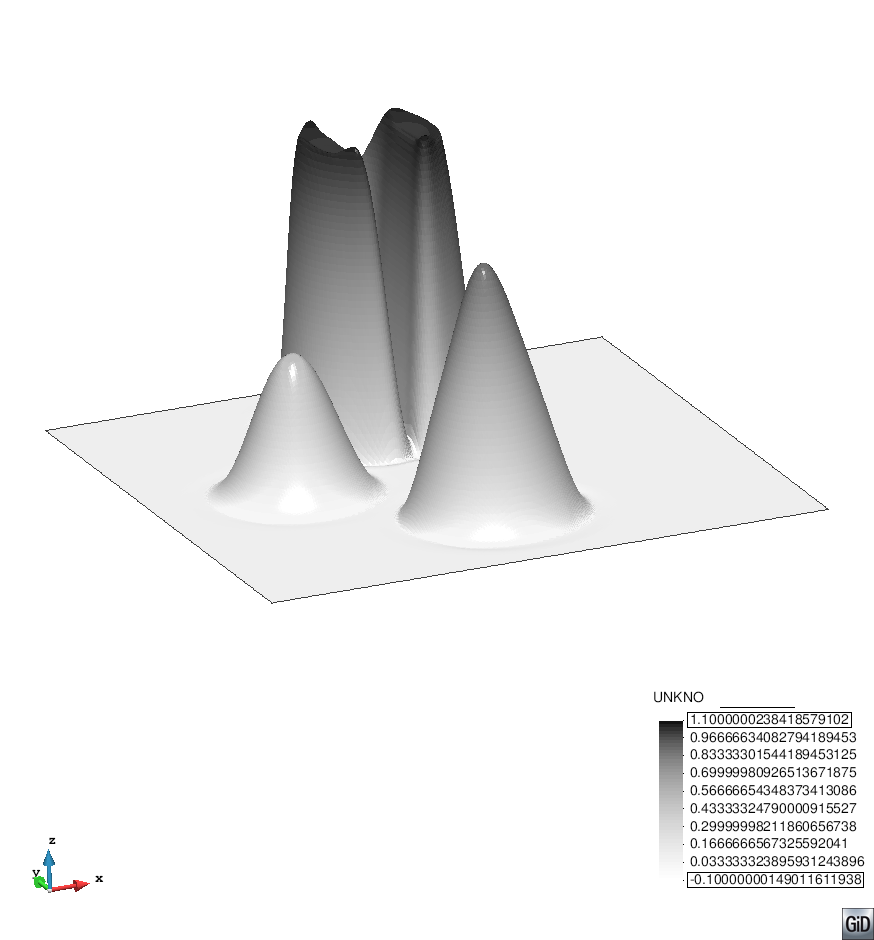
\includegraphics[clip=true, trim=15.5cm 1.1cm 0.9cm 11.65cm, width=1.75cm]{Figures/paper1/15_SZ_GJV_T.png}}%
%\subfigure[{SUPG-bGJV}]{\includegraphics[clip=true, trim=1.6cm 11cm 1.6cm 3cm,width=7.9cm]{Figures/paper1/15_SUPG_GJV_T_001.png}}\\%
%%\subfigure{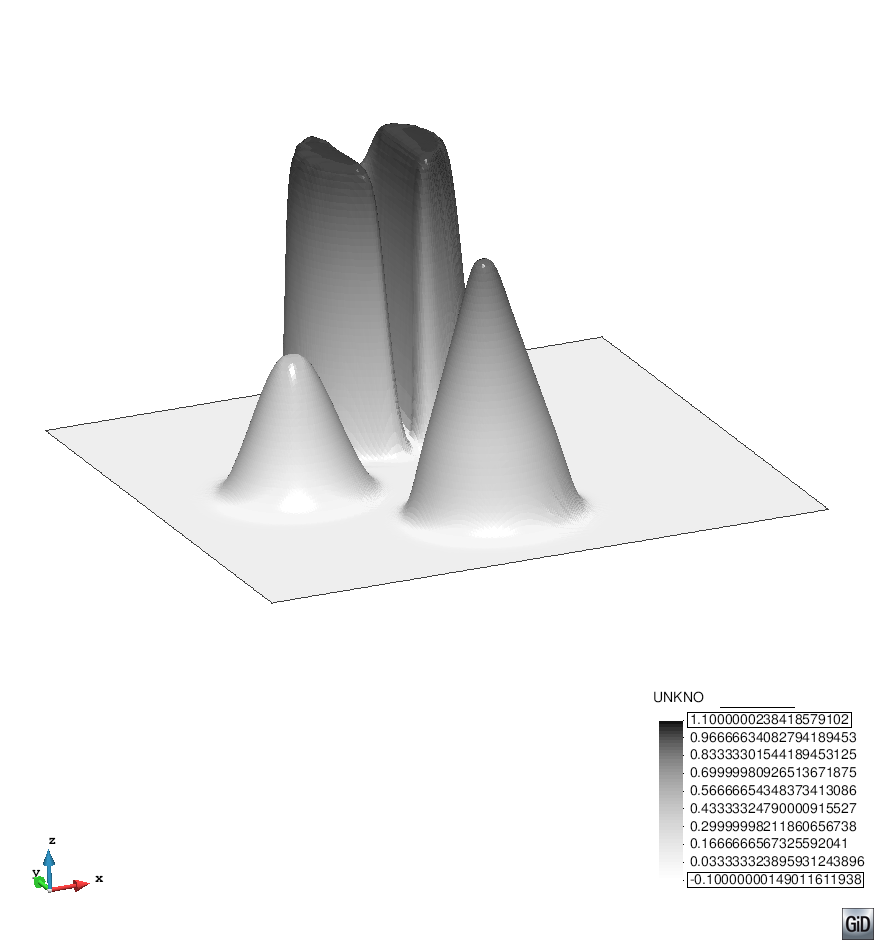
\includegraphics[clip=true, trim=15.5cm 1.1cm 0.9cm 11.65cm, width=1.75cm]{Figures/paper1/15_SUPG_GJV_T.png}}
%\subfigure[{EV}]{\includegraphics[clip=true, trim=1.6cm 11cm 1.6cm 3cm,width=7.9cm]{Figures/paper1/15_None_EV_T_001.png}}%
%%\subfigure{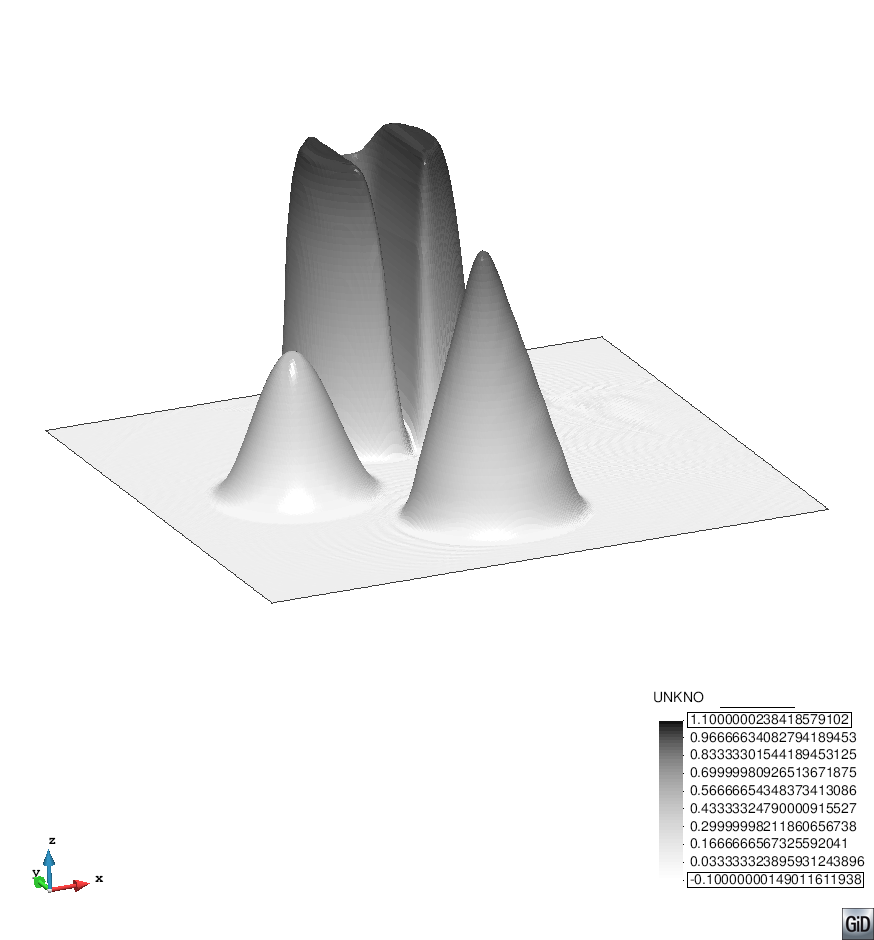
\includegraphics[clip=true, trim=15.5cm 1.1cm 0.9cm 11.65cm, width=1.75cm]{Figures/paper1/15_None_EV_T.png}}\\ %
%\subfigure[{SUPG-RV}]{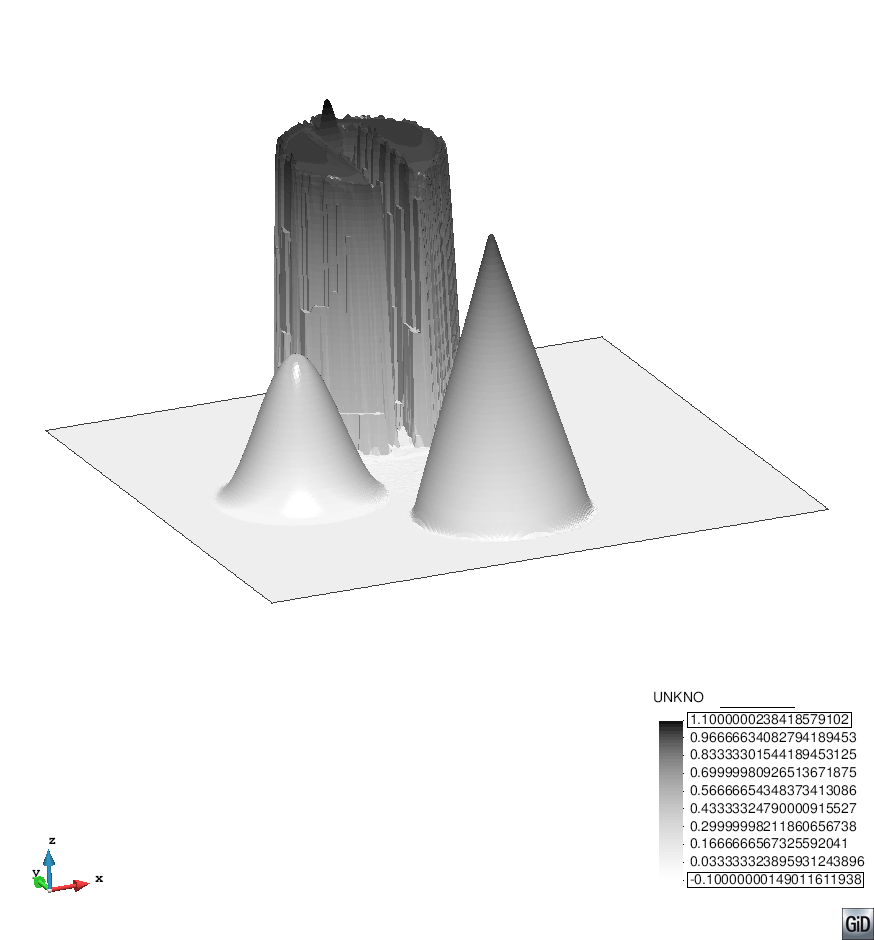
\includegraphics[clip=true, trim=1.6cm 11cm 1.6cm 3cm,width=7.9cm]{Figures/paper1/15_SUPG_RV_T_001.png}}\\%
%%\subfigure{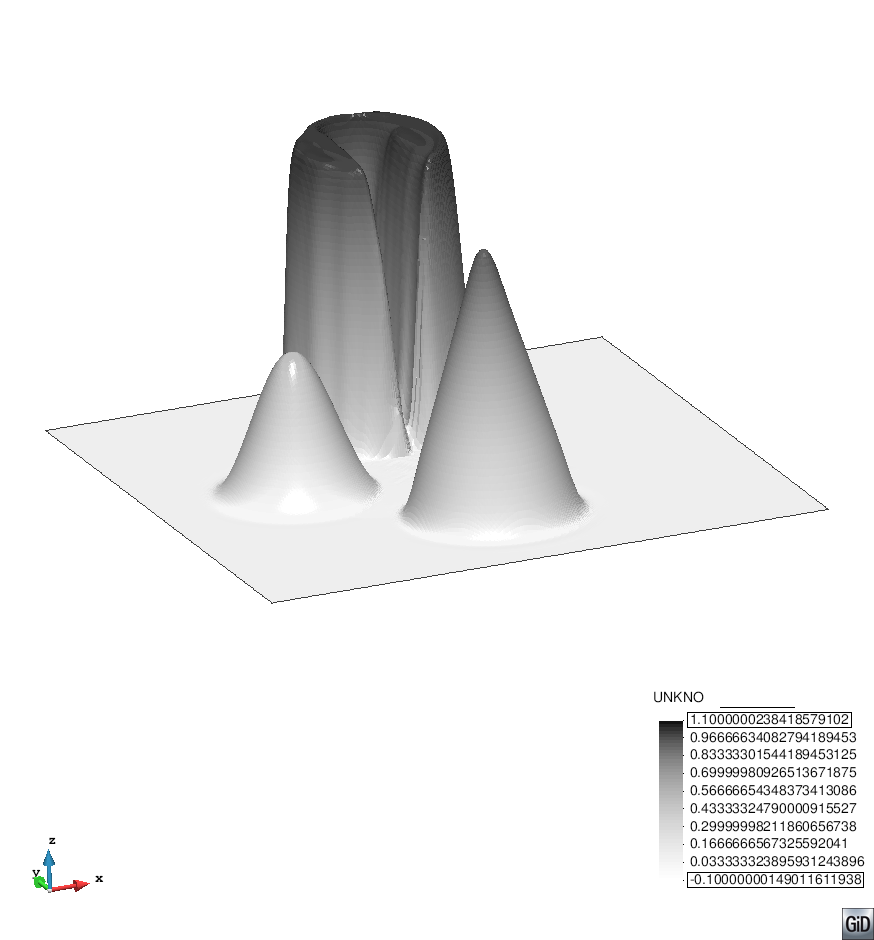
\includegraphics[clip=true, trim=15.5cm 1.1cm 0.9cm 11.65cm, width=1.75cm]{Figures/paper1/15_SUPG_RV_T.png}}\\%
%\subfigure[{nGJV}]{\includegraphics[clip=true, trim=1.6cm 11cm 1.6cm 3cm,width=7.9cm]{Figures/paper1/15_None_PGJV_T_001.png}}%
%%\subfigure{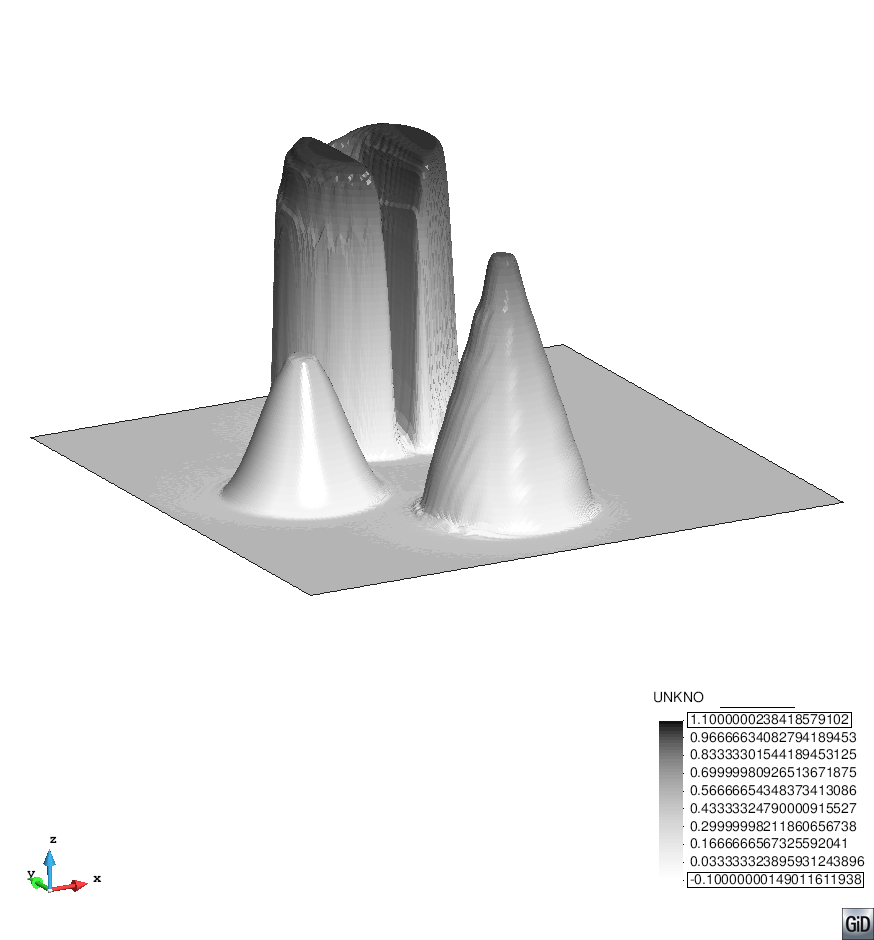
\includegraphics[clip=true, trim=15.5cm 1.1cm 0.9cm 11.65cm, width=1.75cm]{Figures/paper1/15_None_PGJV_T.png}}\\%
%\subfigure[{ wNPS-nGJV}]{\includegraphics[clip=true, trim=1.6cm 11cm 1.6cm 3cm,width=7.9cm]{Figures/paper1/15_SZ_PGJV_T_001.png}}%
%%\subfigure{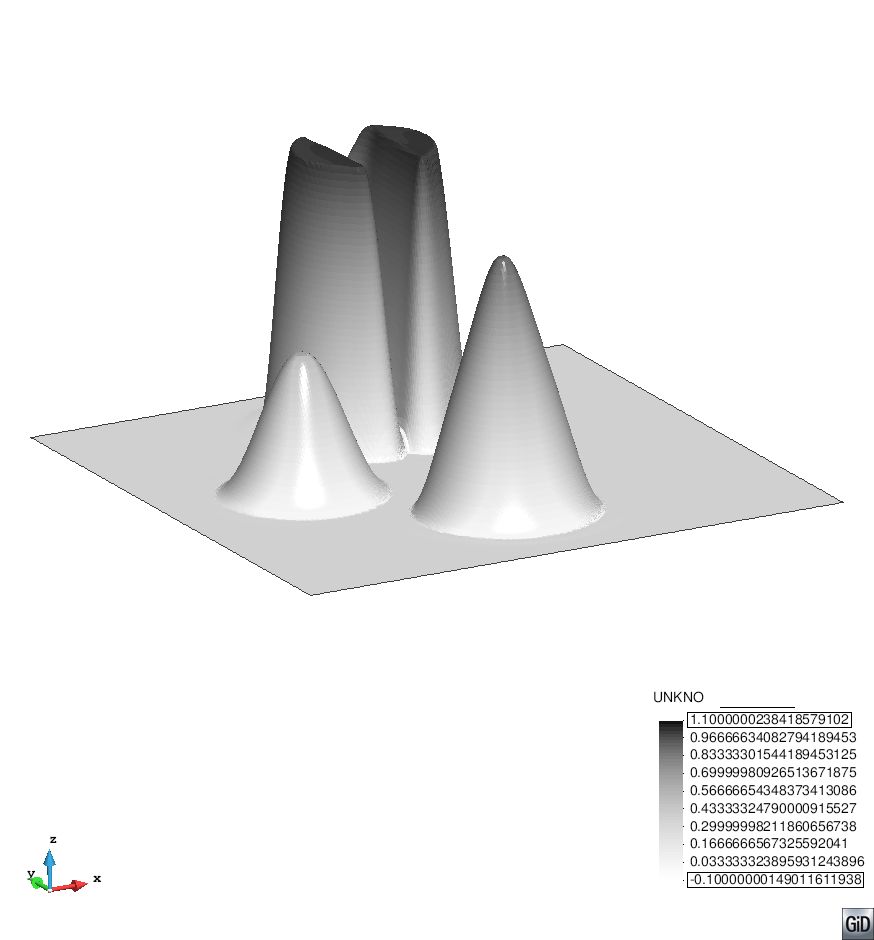
\includegraphics[clip=true, trim=15.5cm 1.1cm 0.9cm 11.65cm, width=1.75cm]{Figures/paper1/15_SZ_PGJV_T.png}}
%\caption{ Test 4. Results $t = 0.01 \, {\rm s}$. Space discretization with $p=1$ and $250\times 250 \times 2$ triangular mesh. Time discretization with Crank-Nicolson, $\Delta t = 2 \cdot 10^{-4}$ and without mass lumping. Results for different schemes at $t = 10^{-2} \, {\rm s}$.}\label{fig-triangle001}
%\end{figure}
%
%

%LES QUATRE PRIMERES

%LES DOS ÚLTIMES


Even when the analysis performed in this work has been done on simplicial meshes, the methods have been tested in quadrilateral meshes also. All the methods provide similar results in both kind of meshes with the notable exception of the bGJV method that, when combined with SUPG stabilization, leads to a very accurate approximation of the solution. The result is plotted in Fig. \Fig{gjvquad}. It is remarkable how the solution keeps the shape of the cylinder and the plateu $u_h=1$. We want to stress that a naive extension of the $1D$ method in \cite{burman_nonlinear_2007}, i.e., the artificial diffusion in \Eq{gjvisc} without the correction term $\frac{\int_e |\nabla u_h \cdot n|{\rm d} \sigma}{\int_e |\nabla u_h| {\rm d} \sigma}$, is extremely over-diffusive. The results after one cycle are displayed in Fig.  \Fig{notuning}. We can observe the dramatic improvement obtained with the correction factor by comparing both plots.


\begin{figure}%
\centering
%\subfigure[{ wNPS-bGJV}]{\includegraphics[clip=true, trim=1.6cm 11cm 1.6cm 3cm,width=7.9cm]{Figures/paper1/15_SZ_GJV_Q.png}}%
%\subfigure{\includegraphics[clip=true, trim=15.5cm 1.1cm 0.9cm 11.65cm, width=1.75cm]{Figures/paper1/15_SZ_GJV_Q.png}}%
\subfigure[{SUPG-bGJV}]{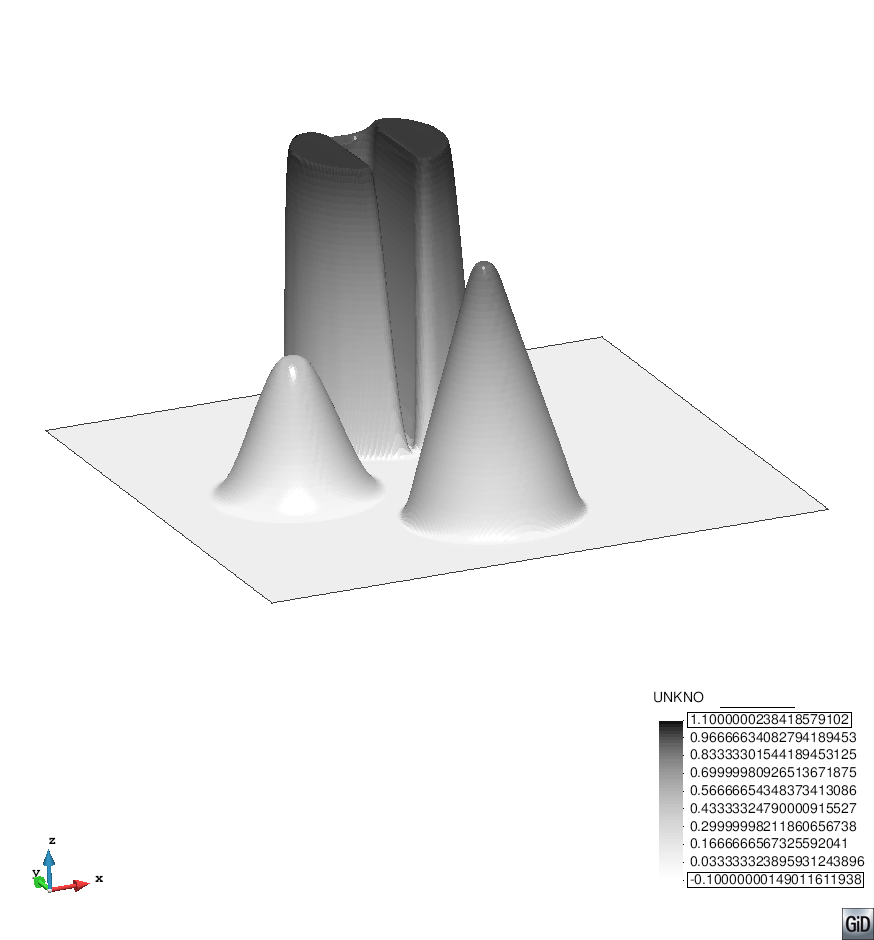
\includegraphics[clip=true, trim=1.6cm 11cm 1.6cm 3cm,width=7.9cm]{Figures/paper1/15_SUPG_GJV_Q.png}\label{fig-gjvquad}}%
\subfigure[{SUPG-bGJV without correction}]{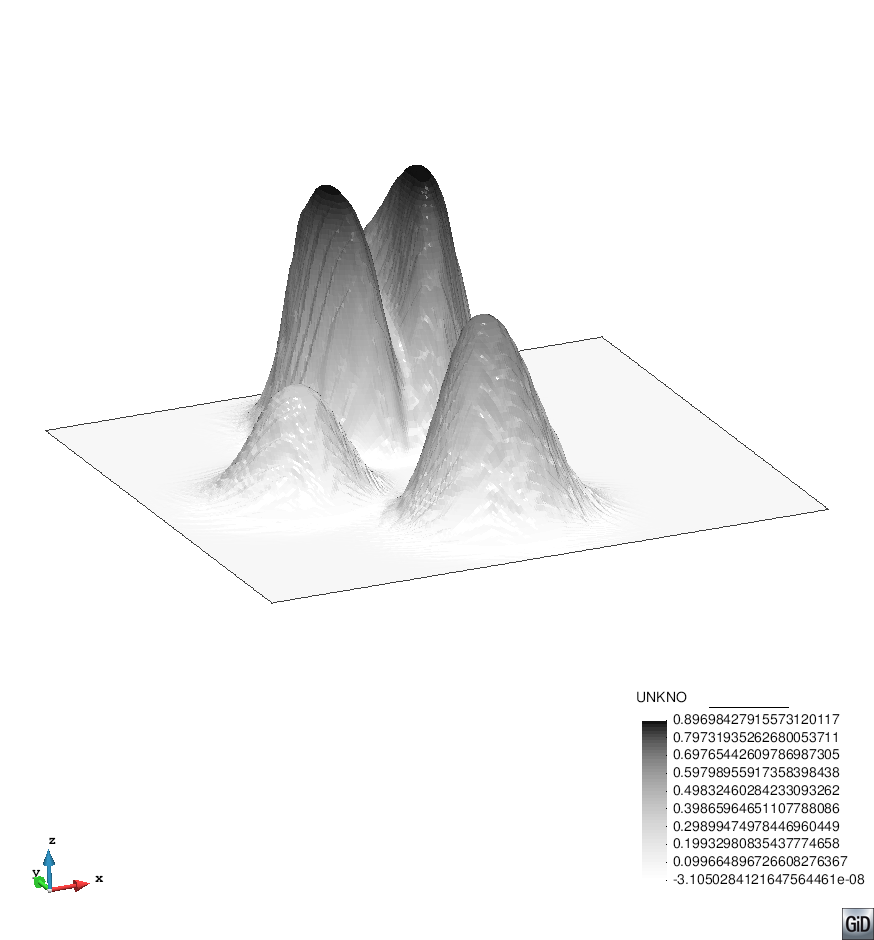
\includegraphics[clip=true, trim=1.6cm 11cm 1.6cm 3cm,width=7.9cm]{Figures/paper1/15_SUPG_GJV_NOtunning.png}\label{fig-notuning}}%
%{\includegaphics[clip=true, trim=25.5cm 1.1cm 0.9cm 23.1cm, width=2cm]{Figures/paper1/15_SUPG_GJV_250_notunning.png}}%
%\subfigure{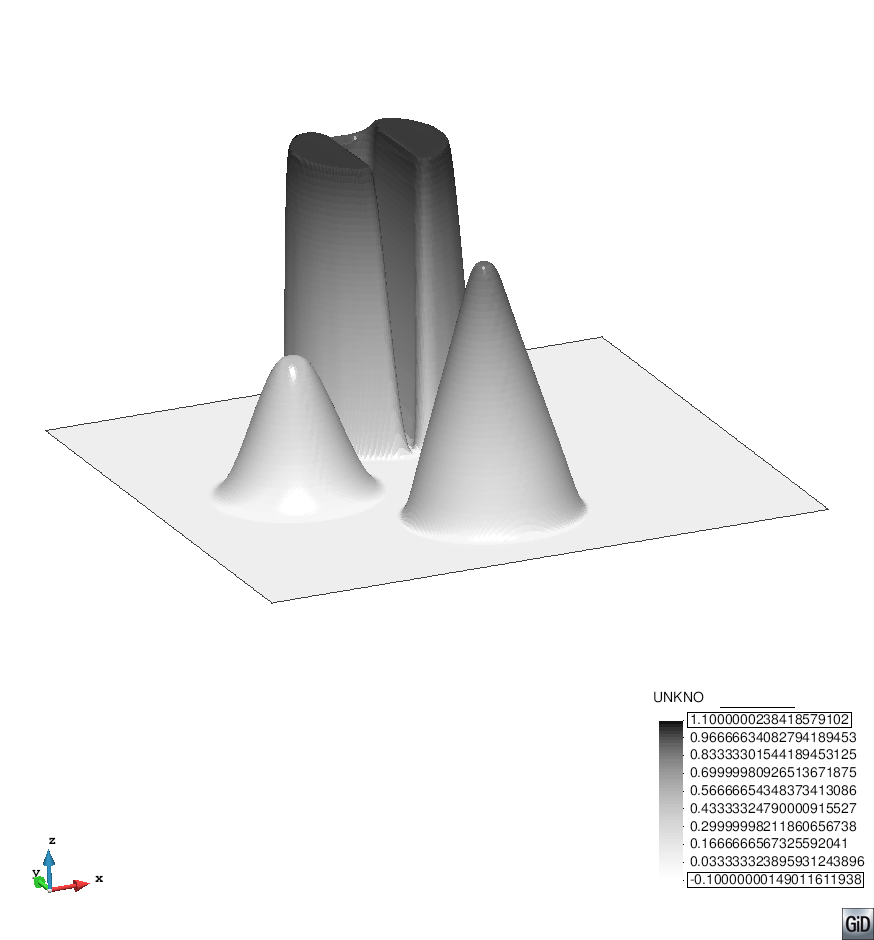
\includegraphics[clip=true, trim=15.5cm 1.1cm 0.9cm 11.65cm, width=1.75cm]{Figures/paper1/15_SUPG_GJV_Q.png}}
%\subfigure[{EV}]{\includegraphics[clip=true, trim=1.6cm 11cm 1.6cm 3cm,width=7.9cm]{Figures/paper1/15_None_EV_Q.png}\label{subf-ev-q-1}}%
%\subfigure{\includegraphics[clip=true, trim=15.5cm 1.1cm 0.9cm 11.65cm, width=1.75cm]{Figures/paper1/15_None_EV_Q.png}}%
%\subfigure[{SUPG-RV}]{\includegraphics[clip=true, trim=1.6cm 11cm 1.6cm 3cm,width=7.9cm]{Figures/paper1/15_SUPG_RV_Q.png}} \\%
%\subfigure{\includegraphics[clip=true, trim=15.5cm 1.1cm 0.9cm 11.65cm, width=1.75cm]{Figures/paper1/15_SUPG_RV_Q.png}}\\%
%\subfigure[{nGJV}]{\includegraphics[clip=true, trim=1.6cm 11cm 1.6cm 3cm,width=7.9cm]{Figures/paper1/15_None_PGJV_Q.png}}%
%\subfigure{\includegraphics[clip=true, trim=15.5cm 1.1cm 0.9cm 11.65cm, width=1.75cm]{Figures/paper1/15_None_PGJV_Q.png}}%
%\subfigure[{ wNPS-nGJV}]{\includegraphics[clip=true, trim=1.6cm 11cm 1.6cm 3cm,width=7.9cm]{Figures/paper1/15_SZ_PGJV_Q.png}}%
%\subfigure{\includegraphics[clip=true, trim=15.5cm 1.1cm 0.9cm 11.65cm, width=1.75cm]{Figures/paper1/15_SZ_PGJV_Q.png}}
\caption{ Test 3. Results $t = 1.0$. Space discretization with $p=1$ and $250\times 250$ quadrilateral mesh. Time discretization with Crank-Nicolson, $\Delta t = 2 \cdot 10^{-4}$ and without mass lumping. Results for different schemes at $t = 1$.}\label{fig-square1}
\end{figure}


%Next, we compare the performance of the bGJV scheme  \Eq{gjvisc} with other shock capturing techniques in Fig. \Fig{SC_kuzmin}. Let us recall that no DMP property has been proved for this method in multidimension. Here we observe that the method that performs better is the SUPG-bGJV method; the EV method does also a good job reducing oscillations but it is still overdissipative. The RV method is the one that shows the largest overshoots and undershoots.
% SB note: Resultats tallats !
%Figs. \Fig{SC_kuzmin}-\subref{SC_kuzmin1} and  \Fig{SC_kuzmin}-\subref{fig-tuning} have been computed with the GJV in \Eq{gjvisc}. 
%% \begin{figure}%
%% \centering
%% \subfigure[{KK-GJV}]{\includegraphics[clip=true, trim=4cm 6cm 4cm 6cm,width=6cm]{Figures/paper1/15_SZ_GJV_250.png}\label{SC_kuzmin1}}%
%% \subfigure{\includegraphics[clip=true, trim=25.5cm 1.1cm 0.9cm 23.1cm, width=2cm]{Figures/paper1/15_SZ_GJV_250.png}}%
%% \subfigure[{ SUPG-bGJV}]{\includegraphics[clip=true, trim=4cm 6cm 4cm 6cm,width=6cm]{Figures/paper1/15_SUPG_GJV_250.png}\label{fig-tuning}}%
%% \subfigure{\includegraphics[clip=true, trim=25.5cm 1.1cm 0.9cm 23.1cm, width=2cm]{Figures/paper1/15_SUPG_GJV_250.png}}
%% \subfigure[{EV }]{\includegraphics[clip=true, trim=4cm 6cm 4cm 6cm,width=6cm]{Figures/paper1/15_None_EV_250.png}\label{SC_kuzmin3}}%
%% \subfigure{\includegraphics[clip=true, trim=25.5cm 1.1cm 0.9cm 23.1cm, width=2cm]{Figures/paper1/15_None_EV_250.png}}%
%% \subfigure[{ SUPG-RV}]{\includegraphics[clip=true, trim=4cm 6cm 4cm 6cm,width=6cm]{Figures/paper1/15_SUPG_RV_250.png}\label{SC_kuzmin4}}%
%% \subfigure{\includegraphics[clip=true, trim=25.5cm 1.1cm 0.9cm 23.1cm, width=2cm]{Figures/paper1/15_SUPG_RV_250.png}}%
%% \caption{ Test 6. Space discretization with $p=1$ and $250\times 250$ mesh. Time discretization with Crank-Nicolson, $\Delta t = 2 \cdot 10^{-4}$ and without mass lumping.}\label{fig-SC_kuzmin}
%% \end{figure}
 

%Now, let us show the behavior of the  nGJV scheme in Algorihtm \ref{alg-wNPS-GJV} on a strictly acute mesh formed entirely by equilateral triangles. To do so we have transformed the domain in a regular hexagon and obtained the results displayed in Fig. \Fig{disasters}. The method shows the DMP property even when no mass lumping is performed. We also tried to implement the edge stabilization proposed in \cite{burman_stabilized_2005} which consists in adding the term \Eq{esterm} with 
%\begin{align}\label{eq-esterm2}
%\psi_K(u_h)|_E = C|\beta|h_K^2|\jump{u_h}_E| \quad \forall E \in \partial K.
%\end{align}
%Since we are using implicit Euler methods for the time integration we need to approximate the absolute value in the following way $|\jump{u_h(t_{n+1})}|\sim {\rm sign}(u_h(t_n))\jump{u_h(t_{n+1})}$. Moreover we have approximated the ${\rm sign}$ functions by the hyperbolic tangent as it is proposed in the original paper. We also used an hexagonal domain as in the previous case so the mesh is stricly acute. Even so, the solution of the problem diverged and turned to be far from acceptable.
%% \begin{figure}%
%% \centering
%% \subfigure[{nGJV alone}]{\includegraphics[clip=true, trim=4cm 6cm 4cm 6cm,width=6cm]{Figures/paper1/15_PGJV_None_hex.png}}%
%% \subfigure{\includegraphics[clip=true, trim=25.5cm 1.1cm 0.9cm 23.1cm, width=2cm]{Figures/paper1/15_PGJV_None_hex.png}}%
%% \subfigure[{ wNPS-nGJV}]{\includegraphics[clip=true, trim=4cm 6cm 4cm 6cm,width=6cm]{Figures/paper1/15_PGJV_SZ_hex.png}\label{fig-dis1}}%
%% \subfigure{\includegraphics[clip=true, trim=25.5cm 1.1cm 0.9cm 23.1cm, width=2cm]{Figures/paper1/15_PGJV_SZ_hex.png}}%
%% \caption{ Test 6. Space discretization with $p=1$ and $38400$ elements mesh. Time discretization with Crank-Nicolson, $\Delta t = 2 \cdot 10^{-4}$ and without mass lumping.}\label{fig-disasters}
%% \end{figure}

%Next, we apply the nGJV method in a non strictly acute mesh and no mass lumping, with the constant $c_{\rm gjv} = \frac{1}{(d+1) \sigma_K \sin(\pi / 6)}$. In this case we cannot guarantee that the method enjoys a DMP, but the results are excellent, as it can be observed in Fig. \Fig{PGJV_kuzmin}. The method does not only eliminate spurious oscillations but is less dissipative than the methods considered in Fig. \Fig{SC_kuzmin} ; observe the thickness of the shock around the square in Fig \Fig{PGJV_kuzmin}\subref{dis1}. In this case we have used a triangular mesh of $250\times250$ square divided in two triangular elements each. The method outperforms all the previous schemes in terms of overshoots and undershoots. In particular, excellent results have been obtained when the shock-capturing scheme \Eq{gjvisc0} is used alone.
%% \begin{figure}%
%% \centering
%% \subfigure[{nGJV alone}]{\includegraphics[clip=true, trim=4cm 6cm 4cm 6cm,width=6cm]{Figures/paper1/15_PGJV_None_250.png}}%
%% \subfigure{\includegraphics[clip=true, trim=25.5cm 1.1cm 0.9cm 23.1cm, width=2cm]{Figures/paper1/15_PGJV_None_250.png}\label{dis1}}%
%% \subfigure[{  wNPS-nGJV}]{\includegraphics[clip=true, trim=4cm 6cm 4cm 6cm,width=6cm]{Figures/paper1/15_PGJV_SZ_250.png}}%
%% \subfigure{\includegraphics[clip=true, trim=25.5cm 1.1cm 0.9cm 23.1cm, width=2cm]{Figures/paper1/15_PGJV_SZ_250.png}}
%% \caption{Test 6. Space discretization with $p=1$ and $250\times 250$ mesh. Time discretization with Crank-Nicolson, $\Delta t = 2 \cdot 10^{-4}$ and without mass lumping.}\label{fig-PGJV_kuzmin}
%% \end{figure}

%% \subsection{Test 8: Steady convective dominant CD problem}
%% Finally we will repeat the test proposed in \cite{john_spurious_2008} which consist in solving the steady convection-diffusion equation
%% \begin{align}\label{steadypbm}
%% -10^{-8} \Delta u + \beta \cdot \nabla u = 0 \quad & \quad {\rm in}\, \Omega=[0,1]\times[0,1]
%% \end{align}
%% with $\beta = (\cos(-\pi/3),sin(-\pi/ 3))$ and boundary conditions
%% \begin{align}\label{steadyic}
%% u_b (x,y) = \left\{\begin{array}{ll}
%% 0 & {\rm if }\, x=1\, {\rm or }\, y\leq 0.75\\
%% 1 & {\rm otherwise.} \\
%% \end{array}\right.
%% \end{align}
%% Since the SC techniques proposed so far have a nonlinear term we must use nonlinear iterations to solve the problem. It was noticed that most of the methods do not converge if nonlinear iterations are applied directly so we have used, as in \cite{john_spurious_2008}, a relaxation parameter $\omega$ in such a way that at each nonlinear time step we solve:
%% \begin{align*}
%% a_h(u_h^k;\tilde{u}_h^{k+1},\phi_h) = 0
%% \end{align*}
%% and then the next iteration is updated as $u_h^{k+1} = u_h^k + \omega(\tilde{u}_h^{k+1} - u_h^k)$.
%% It is well known that the solution of convective dominant problems present sharp layers that induce spurious oscillation in non-stabilized numerical solution. Even when these layers are, strictly speaking, not shocks, the SC methods can detect them and, using the appropriate viscosity, dump the spurious oscillations. In order to compare the performance of different methods we will solve the problem with each of them in different meshes and compute the maximum overshoot and undershoot in each case.
%% Concretelly we will use the SUPG stabilization alone and combined with the GJV in \Eq{gjvisc} with $\nu = 0.5$ and $q=10$, the edge stabilization \Eq{esterm}-\Eq{esterm2} with $C=1$ (ES), the isotropic residual viscosity \Eq{isosc} (RV) with $l_K^{\rm iso} = 0.6$ and $\tau_K^{\rm iso} = 0$ (they were algorithmically optimized) and the crosswind residual diffusion in \Eq{cwsc} (CWRV) with $l_K^{\rm cd} = 0.6$ and $\tau_K^{\rm cd} = 0$. Notice that we cannot implement the Entropy viscosity method in this case since the entropy equation is only defined for transient problems. We also compute the results with the SZ linear stabilization alone and blended with the GJV. The blending in this case consists in taking $\delta_K=0.5 {h_k}{\|\beta\|_{L^\infty(K)}^{-1}} \left(1-\left(\max_{e\in\partial K}  \frac{\jump{|\nabla u_h |}_e}{2  \{|u^h_x|\}_e }\right)^q\right)$ . Results where computed with the relaxation parameter $\omega = 0.1$ and nonlinear tolerance of $10^{-4}$ except for the case SZ+GJV in which we have used $\omega = 0.01$ and $5\cdot 10^{-3}$ because it failed to converge. The edge stabilization method did not converge in any of the cases, it was also tested in a simplicial mesh to check if in that case the results varied but they did not. Results can be found in Tables \ref{t-overs} and \ref{t-unders}. It is clear that the GJV outperforms the rest of the methods, specially when combinated with the SUPG linear stabilization. Eventhough no DMP has been proved for the method it is almost achieved in the result. The results with SUPG stabilization alone and together with the GJV are plotted in Fig. \Fig{Steady}
%% \begin{table}
%% \begin{center}
%% \begin{tabular}{|c|c|c|c|c|c|}
%% \hline Max. Overshoot & $12\times 12$ & $24\times 24$ & $48\times 48$ & $96\times 96$ & $192 \times 192$ \\ 
%% \hline SUPG & 5.57E-1  & 5.59E-1 & 5.59E-1 & 5.59E-1 & 5.59E-1  \\ 
%% \hline SZ & 7.80E-1 & 7.00E-1 & 7.07E-1 & 7.08E-1  & 7.08E-1  \\ 
%% \hline GJV + SUPG & 2.99E-5 &  3.47E-5 & 3.47E-5 & 3.47E-5 & 2.80E-4 \\ 
%% \hline GJV + SZ & 2.62e-2 & 4.06e-2 & 2.61e-2 & 2.60E-2 & 2.61E-2 \\ 
%% \hline ES + SUPG & NC & NC & NC & NC & NC \\ 
%% \hline RV + SUPG & 1.23E-1 & 1.23E-1 & 1.23E-1 & 1.23E-1 & 1.23E-1 \\ 
%% \hline CWRV + SUPG & 2.19E-1 & 2.21E-1 & 2.21E-1 & 2.21E-1 & 2.21E-1 \\ 
%% \hline 
%% \end{tabular} 
%% \label{t-overs}\caption{}
%% \end{center}
%% \end{table}
%% \begin{table}
%% \begin{center}
%% \begin{tabular}{|c|c|c|c|c|c|}
%% \hline Max. Overshoot & $12\times 12$ & $24\times 24$ & $48\times 48$ & $96\times 96$ & $192 \times 192$ \\ 
%% \hline SUPG & -3.93E-2 & -5.57E-2 & -5.567E-2 & -6.055E-2 & -6.05E-2 \\ 
%% \hline SZ & 0 & -2.25E-2 & -3.80E-2 & -4.85E-2 & -5.49E-2 \\ 
%% \hline GJV + SUPG & 0 & 0 & -1.61E-8 & -4.36E-8 & -3.27E-7 \\ 
%% \hline GJV + SZ & 0 & -2.82E-3 & -3.60E-3 & -9.99E-3 & -1.06E-2 \\ 
%% \hline ES + SUPG & NC & NC & NC & NC & NC \\ 
%% \hline RV + SUPG & 2.14E-2 & 2.62E-2 & 2.62E-2 & 2.62E-2 & 2.62E-2 \\ 
%% \hline CWRV + SUPG & -2.48e-2 & 2.93e-2 & 2.93e-2 & 2.93e-2 & 2.93e-2 \\ 
%% \hline 
%% \end{tabular} 
%% \label{t-unders}\caption{}
%% \end{center}
%% \end{table}
%% \begin{figure}%
%% \centering
%% \subfigure[{SUPG}]{\includegraphics[clip=true, trim=1cm 9cm 0.5cm 3cm,width=6cm]{Figures/paper1/96p96_SUPG_None.png}}%
%% \subfigure{\includegraphics[clip=true, trim=25.5cm 1.1cm 0.9cm 23.1cm, width=2cm]{Figures/paper1/96p96_SUPG_None.png}}%
%% \subfigure[{ GJV + SUPG}]{\includegraphics[clip=true, trim=1cm 9cm 0.5cm 3cm,width=6cm]{Figures/paper1/96p96_SUPG_GJV.png}}%
%% \subfigure{\includegraphics[clip=true, trim=25.5cm 1.1cm 0.9cm 23.1cm, width=2cm]{Figures/paper1/96p96_SUPG_GJV.png}}
%% \caption{ Test 8. $p=1$. Mesh $96\times 96$. $\omega = 0.1$. ${\rm TOL} = 10^{-4}$. NO Mass lumping.}\label{fig-Steady}
%% \end{figure}




%\input 00_numericalexamples.tex

%
%% \section{Some numerical analyses}
%% %
%% From the error analysis, taking as interpolant of the exact solution $u$ the $L^2$ projection with optimal
%% interpolation properties $\pi_h(u)$, and denoting $i=u-\pi_h(u) \in V_h^\perp$ (interpolation error) and $e_h = u_h -\pi_h(u) \in V_h$, we have:
%% $$
%% (\beta \cdot \nabla i,e_h) = - (i,\beta \cdot \nabla e_h) = - (i, \pi_h^\perp (\beta \cdot \nabla e_h) ) \leq \| i \|  \| \pi_h^\perp (\beta \cdot \nabla e_h) \|,%\leq \frac{|\beta|_{L^\infty(\Omega)}}{h} \|i \| + \frac{h}{|\beta|_{L^\infty(\Omega)}}\| \pi_h^\perp (\beta \cdot \nabla e_h)\|.
%% $$
%% where we have used the fact that $\beta$ is solenoidal and I have not considered boundary conditions (put it). We easily get:
%% $$
%% \| \pi_h^\perp (\beta \cdot \nabla e_h)\| \leq \| \kappa_h^\perp (\beta \cdot \nabla e_h)\| \leq \| \kappa_h^\perp (\beta_h \cdot \nabla e_h)\| + 
%% \| \kappa_h^\perp (\beta_h^\perp \cdot \nabla e_h)\|,
%% $$
%% where $\beta_h$ is an approximation of $\beta$ in $V_h^1$ (linear FE space) such that $\|\beta_h^\perp\|_{L^\infty(\Omega)} \lesssim h \|\beta \|_{W^{1,\infty}(\Omega)}$, where $\beta_h^\perp = \beta - \beta_h$. It holds for $\beta_h$ being the Scott-Zhang projector \cite{}. We can easily check that $\kappa^\perp_h (\beta_h \cdot \nabla e_h) = \beta_h \cdot \kappa_h^\perp(\nabla e_h)$ at every node of $K \in \mathcal{T}_h$. Further, $\kappa^\perp_h (\beta_h \cdot \nabla e_h)|_K \in V_h^k(K)$ (the restriction of $V_h$ onto $K$) and so $\kappa^\perp_h (\beta_h \cdot \nabla e_h) = \rho_{h,K}(\beta_h \cdot \kappa_h^\perp(\nabla e_h))$ on $K$, where $\rho_{h,K}$ is the nodal (Lagrangian) interpolant in element $K$. As a result, using the stability of the Lagrangian interpolant, we have that $\|\kappa^\perp_h (\beta_h \cdot \nabla e_h)\| \lesssim \|\beta_h \cdot \kappa_h^\perp(\nabla e_h)\| \lesssim \| \beta \cdot \kappa_h^\perp(\nabla e_h)\| + \| \beta_h^\perp \cdot \kappa_h^\perp(\nabla e_h)\|$. Further, using an inverse inequality and the interpolation properties of $\beta_h$ we have,
%% $$
%% \| \beta_h^\perp \cdot \kappa_h^\perp(\nabla e_h)\| + 
%% \| \kappa_h^\perp (\beta_h^\perp \cdot \nabla e_h)\| \lesssim \|\beta \|_{L^{\infty}(\Omega)} \|\nabla e_h\|
%% \lesssim \|\beta\|_{W^{1,\infty}(\Omega)} \|e_h\|.
%% $$
%% Combining these results we get
%% $$
%% (\beta \cdot \nabla i,e_h) \lesssim \|i \| ( \| \beta \cdot \kappa_h^\perp(\nabla e_h)\| +  \|\beta\|_{W^{1,\infty}(\Omega)} \|e_h\|) \lesssim (\delta_*^{-\half} \|i\| )( \delta^\half \| \beta \cdot \kappa_h^\perp(\nabla e_h)\| + h^\half \|e_h\|)
%% $$
%% where $\delta^{- \half}_* = h^{- \half} (\|\beta\|_{W^{1,\infty}(\Omega)} + \|\beta\|^\half_{L^{\infty}(\Omega)})$ and $\delta = h \|\beta\|^{-1}_{L^{\infty}(\Omega)} \lesssim h_K \|\beta\|^{-1}_{L^{\infty}(K)}= \delta_K$.
%% Using the Gronwall lemma we can end the convergence proof.
%



\section{Conclusions}\label{s-concl}
%
In this work, we propose a novel linear stabilization technique for continuous FE
discretizations of time-dependent transport problems which belongs to the family of local 
projection stabilization techniques. In particular, we consider a Scott-Zhang-type projector which is 
well-defined for $L^1(\Omega)$ functions, extending the ideas in \cite{badia_stabilized_2012} to convection stabilization. 
Stability and numerical analyses for the linear transport problem are carried out. 

Further, we design a weighting of the aforementioned linear stabilization such that, 
%blending of the aforementioned linear and nonlinear stabilization and prove that 
when combined with a FE discretization with a DMP (usually
attained via a shock-capturing technique), it does not spoil the monotonicity properties. 
%the combined formulation satisfies all the properties of the nonlinear stabilization alone. 
%Thus, the linear stabilization proposed in this paper can be defined in such
%a way that it does not spoil the DMP property and converges to entropy solutions. 
It is attained by switching off the linear stabilization around shocks.

Next, we have proposed different nonlinear stabilization (shock-capturing) schemes based on 
artificial viscosity, in order to reduce or even eliminate local oscillations around shocks/discontinuities. 
In particular, we have used a definition of the artificial viscosity based on boundary gradient jumps (bGJV),
following the original work of Burman in \cite{burman_nonlinear_2007}, and another one based on
nodal jumps (nGJV). For the nodal method, we have proved a salient strong DMP property for multidimensional 
time-dependent transport problems.%and converge to entropy solutions for the one-dimensional Burgers' equation. 


Finally, a complete set of numerical experiments is included. On one hand, we check experimentally
the theoretical monotonicity properties of the weighting formulations and the nonlinear stabilization. Next, gradient-jump shock-capturing methods (with different linear stabilizations) are compared against residual-based and entropy-based formulations, in order to show its performance. The results obtained with the nGJV scheme are remarkably good, with oscillation-free solutions in different tests.

Future work will be the extension of GJV methods to high order and/or discontinuous Galerkin formulations.
Further, since these methods do not rely on entropy functions, they can
also be extended to CDR problems, in order to properly capture boundary and internal layers.  

\chapter{Monotonicity preserving methods for discontinuous Galerkin method}
\label{chap-paper2}

\section{Introduction}

It is well known that the operator $L$ associated to an elliptic problem such as the convection-diffusion problem enjoys the maximum property, meaning that the maximum (resp., minimum) of the solution to the problem $Lu=f$ is achieved on the boundary of the domain if the source term, $f$, is negative (resp., positive). 
%Moreover, under certain extra regularity conditions, the operator enjoys the strong maximum principle meaning that the solution has no local maximum (resp., minimum) in the interior of the domain if $f\leq 0$ (resp., $f\geq 0$) .
In particular, this property ensures that the solution of the problem will not show oscillations. It is well known that the solution of a convection-dominated problem may present sharp layers that may induce spurious oscillations in the discrete approximation of the solution. We are interested in finding a method that ensures a similar maximum property at the discrete discontinuous level in order to obtain a method that gives oscillation free solutions.

When the problem is discretized, this maximum property may be inherited by what is called \textit{discrete maximum principle} (DMP). Several definitions of the DMP have been proposed in the literature for continuous discrete approximations (see \cite{codina_discontinuity-capturing_1993,hohn_remarks_1981,varga_discrete_1966,burman_edge_2004,roos2008robust}). Some of them are equivalent while some others are weaker or stronger. There is also a lot of literature about the conditions on the mesh for the Poisson problem to enjoy the DMP \cite{hohn_remarks_1981,vejchodsky_discrete_2007,horvath_discrete_2013,payette_performance_2012} as well as discrete methods specially implemented to fulfil such property. Methods have been designed for linear finite differences \cite{ciarlet_discrete_1970} and continuous linear finite elements \cite{ciarlet_maximum_1973,codina_discontinuity-capturing_1993,mizukami_petrov-galerkin_1985,burman_discrete_2004,burman_edge_2004,burman2005stabilized}. {These methods are implicit in sense, and usually based on the addition of AV to the problem at hand; they are traditionally called shock (or discontinuity)-capturing techniques, even though we favour the notation \emph{nonlinear stabilization}.} 
%There is also a interesting simple approach to the problem given by Kreuzer \cite{kreuzer_note_2012} consisting on applying a simple cutoff to the solution but it can not be applied in an implicit code and moreover it only works when the maximum and the minimum of the problem are known beforehand. 
Some approaches to prove a DMP using piecewise higher order polynomials have been done \cite{nagarajan_enforcing_2011,payette_performance_2012,kuzmin_design_2008,vejchodsky_discrete_2007,vejchodsky_higher-order_2010,yanik_discrete_1987,yanik_sufficient_1989} but only the Poisson problem has been proved to enjoy the DMP and only on certain one-dimensional (1D) meshes \cite{vejchodsky_discrete_2007} and on very restrictive quadratic and cubic two dimensional meshes \cite{lorenz_zur_1977,hohn_remarks_1981}. When it comes to discontinuous methods, most of the shock capturing techniques are based on the concept of slope limiter, proposed by Cockburn and Shu for conservation laws \cite{cockburn_rungekutta_1998,cockburn_runge-kutta_1990} and latter adapted to the convection-dominated convection-diffusion problem  \cite{cockburn_rungekutta_2001}. The same strategy can be applied to finite volume methods (see \cite{zhang_maximum-principle-satisfying_2010,zhang_maximum-principle-satisfying_2011,zhang_maximum-principle-satisfying_2012}). Again, these methods consist in a postprocess after the solution is computed and are designed for explicit methods. {However, as far as we know, there are no works dealing with nonlinear stabilization and implicit DMP-preserving dG formulations. In fact, even the definition of what a DMP for dG means is open.}

Concerning to the study of the DMP for the Poisson problem in the dG setting, there is {only} one work by Horv\'ath and Mincsovics \cite{horvath_discrete_2013}; they analyse the fulfilment of certain condition on the stiffness matrix $\mathbf{K}$ that ensure the following property for the 1D interior penalty (IP) method:
\begin{align*}
\mathbf{Ku}\leq 0 \quad \Longrightarrow   \quad \max \mathbf{u} \leq \max\{0,\max \mathbf{u}_{\partial \Omega}\}. 
%\quad \forall u\in\mathbb{R}^{N_h}%\mathcal{C}^2({\Omega})\cap\mathcal{C}(\bar{\Omega}).
\end{align*} 

{The aim of this work is twofold. On one side, we propose a new (variational) definition of the DMP for dG, {and we prove that it is a sufficient condition to have the the minimum/maximum (depending on the sign of the forcing term) on the boundary for multidimensional problems}. The new definition is stronger than the one given in \cite{horvath_discrete_2013} and it is, in some sense, closer to the one used in \cite{burman_nonlinear_2007} for the 1D continuous Galerkin (cG) discretization of the Burgers' equation. On the other hand, we construct a multidimensional nonlinear stabilization based on AV for dG methods and prove that, when restricted to the 1D case, the nonlinear stabilization combined with an incomplete (or weighted) IP dG method with upwinding is capable to ensure our DMP for the discrete dG solution of \Eq{strongform}. In any case, numerical experiments evindence that the method also satisfies the DMP in the multidimensional case.}


The outline of the article is the following. In Section \ref{s-contprob} we introduce the continuous convection-diffusion problems and its Galerkin discretization using finite elements. The IP dG method for the Laplacian is presented in Section \ref{s-ip}. Our novel definition of the DMP for the dG scheme is proposed in Section \ref{s-dmp} and some good properties derived from it are stated. Moreover, in Subsection \ref{ss-dmp}, we prove that the IP method for the Laplacian enjoys the DMP in the 1D case. The extension of the IP method for the convection-diffusion problem  is given in Section \ref{s-cd}. In Section \ref{s-ad}, an AV technique is proposed for the 1D case, and we prove that it satisfies the DMP. Further, we extend the method to the multidimensional case. Numerical experiments are included in Section \ref{s-numex}. Finally, some conclusions are drawn in Section \ref{s-concl}.


\section{Weak Form and Notation}\label{s-contprob}


We will consider the convection-diffusion problem with Dirichlet boundary conditions:
\begin{equation}
\label{eq-strongform}
\left\{
\begin{array}{rcll}
Lu:=  - \nabla\cdot(\mu \nabla u) + \nabla\cdot(\beta u)  &=& f & \rm{in}\ \Omega, \\
u&=&g & \rm{on}\ \partial\Omega.\\
\end{array}\right.
\end{equation}
We assume that $\mu\in L^2(\Omega)$ and $\beta\in H^1(\Omega)\cap C^0(\Omega)$ is solenoidal ($\nabla \cdot \beta = 0$). It is well known that the operator $L$ associated to problem \Eq{strongform} enjoys the maximum principle (for proofs on maximum principles for elliptic problems see \cite{gilbarg2001elliptic}). 
\begin{definition}
We say that an operator $L$ posseses the maximum principle if, for all $u\in\mathcal{C}^2(\Omega)\cap\mathcal{C}(\bar{\Omega})$, the following implication holds:
\begin{align*}
Lu\leq 0 \quad \textrm{in}\quad \Omega  \quad \Longrightarrow   \quad \max_{{S}} u \leq \max_{\partial S} u\quad \forall S\subset \Omega.
%Lu\geq 0 \quad \textrm{in}\quad \Omega  \quad \Longrightarrow   \quad \max_{\bar{\Omega}} u \geq \max\{0,\max_{\partial \Omega} u\}
\end{align*}
\end{definition}

Before studying how to achieve a maximum principle at the discrete level for the convection-diffusion problem, we will focus on the rather simpler Poisson's equation:
\begin{equation}
\label{eq-spoisson}
\left\{
\begin{array}{rcll}
\displaystyle - \Delta u & = & f & \rm{in}\, \Omega \\
u&=&g &\rm{on}\, \partial\Omega.\\
\end{array}\right.
\end{equation}
We denote by $(\cdot,\cdot)_K$ the $L^2(K)$ inner product for any $K\subset \Omega$ and by $(\cdot,\cdot)$ the $L^2(\Omega)$ product. We consider $(\cdot,\cdot)_h$ the $L^2(\Omega)$-scalar product evaluated using nodal quadrature (corresponding to the lumped mass matrix). The bilinear form $a(\cdot,\cdot)$ associated to the problem \Eq{spoisson} is $a(u,v) = ( \nabla u,\nabla v)$. So, the weak form of \Eq{spoisson} reads as: 
\begin{equation}
\label{weakform}
\textrm{{Find $u\in H^1(\Omega)$ such that }} a(u,v)=(f,v) \quad \forall v \in H^1(\Omega).
\end{equation}
Let us consider partitions $\thn = \{K\}$ of $\Omega$ formed by simplicial elements $K$ of characteristic length $h_K$; we denote by $h$ the characteristic size of the mesh. The corners of the mesh will be denoted by $x_i$, $i=1,\cdots, N_h$ ($N_h$ being the total number of corners), and the macroelement associated to $x_i$ will be designated by $\Omega_i = \cup_{x_i\in  K}K$. %defined by $\thn=\left\{K_i=[x_{i-1},x_i] \textrm{;   } i=1,\cdots ,N\right\}$ with $a=x_0<x_1<\cdots<x_i<\cdots<x_N=b$ and $h_i=x_i-x_{i-1}$. %We assume that the mesh is such that $\rho = \max\{\frac{h_i}{h_j}|K_i\cap K_j\neq\emptyset\}$ is bounded. Given $x_i$, we call macroelement $\Omega_i$ to the union of the elements that are adjacent to $x_i$, $\Omega_i=K_i\cup K_{i+1}$. In order to fix the notation we define the reference element $\hat{K}=[-1,1]$ and the bijective linear mapping, $F_i$, between $\hat{K}$ and the $i$-th element $K_i$, defined by $F_i(x) = x_{i-1}+\frac{x+1}{2}h_i$. Finally we denote by $\mathbb{P}_k$ the space of polynomials of degree at most $k$ in $\hat{K}=[-1,1] $. 
 The discrete space considered henceforth is the discontinuous space of piecewise linear functions $ \vh=\{v_h \, | \, v_h|_K \in \mathbb{P}_1(K)$ $\forall K\}$.  %$\vh=\{v_h | F^{-1}_i(v_h|_{K_i})\in \mathbb{P}_1$ $\forall i\}$. This means that the solutions can be expressed in terms of a finite basis $\{\phi_j\}_{i=1}^{N_h}$ where $N_h=2N$ in this case:
%\begin{equation}
%u_h(x)=\displaystyle\sum_{j=1}^{N_h} u_j\phi_j(x), \quad x\in \Omega
%\end{equation}%
%Moreover we can adapt the previous bilinear forms to this finite dimensional space. We define $a_h$, $A_h^s$ and $l_h$ as the trivial restrictions of $\bar{a}$, $A_s$ and $l$ on $\mathcal{V}_h$.
%
%
%The FEM consists of solving the following problem:
%
%
%\begin{equation}
%\label{discweakform}
%\textrm{\emph{Find $u_h\in \mathcal{V}_h$ such that }} A_h^s(u_h,v_h)=l_h(v_h) \quad \forall v_h \in \mathcal{V}_h.
%\end{equation}
%
%
%Finally, we define the mass matrix $\textbf{M}=(m_{ij})$ and the matrix $\textbf{A}=(a_{ij})$ by
%
%\begin{center}
%
%\begin{tabular}{ccc}
%$m_{ij}=(\phi_i,\phi_j)$ & and & $a_{ij}=a_h(\phi_i,\phi_j),$
%\end{tabular}
%\end{center}
%
%
%and $\textbf{f}=(f_i)$, with $f_i=(f,\phi_i)$. Then, (\ref{discweakform}) can be expressed in the following matrix form:
%
%\begin{center}
%
%\begin{equation}
%\label{matweakform}
%\textrm{\emph{Find $\textbf{u}(s)\in \mathbb{R}^{N_h}$ such that }} \textbf{M} \partial_t \textbf{u}(s)+\textbf{A} \textbf{u}(s) = \textbf{f}(s).
%\end{equation}
%\end{center}
%
%Concretely, for each point $x_i$ we define the pair of nodes, $x_i^+$ and $x_i^-$, such that $u_h(x_i^\pm) = \lim_{\varepsilon\rightarrow0+} u_h(x_i \pm \varepsilon)$. In the same vein we can define $K_{i,\pm} $ as the element that contains $x_i^\pm$ ($K_{i,-} = K_{i}$ and $K_{i,+}=K_{i+1}$). Then, we define $\varphi_i^\pm$ as the linear nodal shape function corresponding to $x_i^\pm$, that is $\varphi_i^\pm(x_i^\pm)=1$, $\varphi_i^\pm(x_i^\mp)=0$ and $\varphi_i^\pm(x_j^\alpha)=0$ $\forall j\neq i$, $\forall \alpha\in\{-,+\}$. It is clear that the support of $\varphi_i^\pm$ is $K_{i,\pm}$ and that we can define $\phi_j = \varphi_{(j-1)/2}^+$ for odd values of $j$ and $\phi_j=\varphi_{i/2}^-$ for even values of $j$ in such a way that 
%\begin{equation}
%u_h(x)=\displaystyle\sum_{i=1}^{N} u_h(x_{i-1}^+)\varphi_{i-1}^+(x) + u_h(x_{i}^-)\varphi_{i}^-(x), \quad x\in \Omega
%\end{equation}
Let $\mathcal{E}_h = \cup_{K \in \mathcal{T}_h^N} \partial K$    %\{F\}$ 
be the set of the facets of the mesh and $\mathcal{E}_h^0=\mathcal{E}_h\backslash\partial\Omega$. We define $T(\mathcal{E}_h)=\prod_{K\in \mathcal{T}_h^N} L^2(\partial K)$. The functions in $T(\mathcal{E}_h) $ are double-valued on $\mathcal{E}_h^0$ and single-valued on $\partial \Omega$; in particular, $V_h|_{\mathcal{E}_h} \subset T(\mathcal{E}_h)$. The functions $v_h\in\vh$ can be expressed as a linear combination of the basis $\{\varphi_i^K\}$ where $\varphi_i^K$ is defined for all pairs $\{i,K\}\in \{1,\cdots,N_h\} \times \thn$ such that $x_i\in K$.  $\varphi_i^K$ corresponds to the discontinuous function that is linear in $K$, with $\varphi_i^K(x_i) = 1$ and $\varphi_i^K(x_j)=0$ for $x_j\in K$, $j\neq i$, and  $\varphi_i^K = 0$ for $x\in\Omega\setminus K$. So, a function $v_h\in\vh$ would read as:
\begin{align*}
v_h(x) = \sum_{i=1}^{N_h} \sum_{K\subset \Omega_i} u_i^K \varphi_i^K (x),\qquad \forall x\in \Omega.
\end{align*}
Moreover we can define the solution in a single element $K$ as $u^K_h (x) = \sum_{x_i\in K} u_i^K \varphi_i^K (x)$, $\forall x\in K$, and its constant  gradient $\nabla u^K_h = \sum_{x_i\in K} u_i^K \nabla \varphi_i^K|_K $. %Given an interior point $x_i\in\mathcal{E}_h^0$ and the corresponding surrounding elements $K_{i,-},K_{i,+}\in \mathcal{T}_h^N$, we know that the unit normal vectors on $x_i$ pointing exterior to $K_{i,-}$ and $K_{i,+}$ are $n_i^-=1$ and $n_i^+=-1$ respectively. 
For any facet $F\in\mathcal{E}_h^0$ we know there are only two elements, say $K_F^+$ and $K_F^-$, such that $\partial K_F^+\cap \partial K_F^- = F$. In addition, we can name $n_F^+$ and $n_F^-$ the unitary normal to face $F$ outside $K_F^+$ and $K_F^-$, respectively.  Given $q\in T(\mathcal{E}_h)$,  we can define the common concepts of average $\mean{\cdot}$ and jump $\jump{\cdot}$ on an interior point $x$ of a facet $F\in \mathcal{E}_h^0$ as follows: $$\mean{q}(x)=0.5(q^{K_F^+}(x)+q^{K_F^-}(x)),\quad \jump{q}(x) = q^{K_F^+}(x)n_F^++q^{K^-_F}(x)n_F^-. $$ We also define the harmonic average of $q$ on $x$ as $\meanhar{q}(x) = (2q^{K_F^+}(x)q^{K_F^-}(x))/(q^{K_F^+}(x)+q^{K_F^-}(x))$. On boundary points $x\in\partial\Omega$, we define $\mean{q}(x)=q(x)$, $\jump{q}(x) = q(x) n_{\partial\Omega}(x)$ and $\meanhar{q} (x) = q(x)$.  %\frac{2q^{K_F^+}q^{K_F^-}(x)}{q^{K_F^+} + q^{K_F^-}(x)}$.

\section{The Interior Penalty Method for the Poisson's Problem}\label{s-ip} There are numerous dG methods in the literature to approximate the Poisson problem. Many of them are contained in the unified analysis carried out by Arnold \emph{et al.} in \cite{arnold_unified_2002}, where they conclude that any dG method approximating the second-order elliptic problem $-\Delta u = f$ uses the following bilinear form:
%\begin{align*}
%a_h(u_h,v_h) = \int_\Omega  u_{h,x} v_{h,x} + \sum_{x_i\in\mathcal{E}_h} (\jump{\tilde{u}-u_h}_i\mean{ v_{h,x}}_i - \mean{\tilde{\sigma}}_i \jump{v_h}_i) + \sum_{x_i\in\mathcal{E}_h^0} (\mean{\tilde{u}-u_h}_i\jump{ v_{h,x}}_i - \jump{\tilde{\sigma}}_i \mean{v_h}_i),
%\end{align*}
\begin{align*}
a_h(u_h,v_h) = \int_\Omega  \nabla u_{h} \nabla v_{h} + \int_{\mathcal{E}_h} (\jump{\tilde{u}-u_h}\mean{ \nabla v_{h}} - \mean{\tilde{\sigma}} \jump{v_h}) + \int_{\mathcal{E}_h^0} (\mean{\tilde{u}-u_h}\jump{ \nabla v_{h}} - \jump{\tilde{\sigma}} \mean{v_h}),
\end{align*}
where $\tilde{u}=\tilde{u}(u_h)$ and $\tilde{\sigma}=\tilde{\sigma}(u_h)$ are  scalar numerical fluxes that approximate $u$ and $\nabla u$ respectively on the boundaries of the elements. Different choices for these fluxes lead to different dG methods. We consider the IP method, which consists in taking 
\begin{align*}
\tilde{u} = \mean{u_h} + \xi n_K\cdot\jump{u_h}, & &  \tilde{\sigma} = \mean{\nabla u_{h}} - C_1 \jump{u_h}.
\end{align*}
Given a facet $F$, the value $C_1(x)=c^{ip} \tilde{h}^{-1}$ for any $x \in F$, where $c^{ip}|_F=c^{ip}_F$ is a facet constant to be chosen and $\tilde{h}|_F = h_F := \min_{\bar{K} \supset F}\{h_K\}$. The parameter $\xi$ can take values $\xi=0,0.5$ or $1$, leading to the symmetric, incomplete, or nonsymmetric IP method, respectively:
%\begin{align}\label{eq-muIP}
%a_h = \int_\Omega  u_{h,x} v_{h,x} +\sum_{x_i\in\mathcal{E}_h} [(2\xi-1)\jump{u_h}_i\mean{ v_{h,x}}_i - \mean{u_{h,x}}_i \jump{v_h}_i + c^{ip}_{i} \bar{h}_i^{-1}\jump{u_h}_i\jump{v_h}_i]
%\nd{align}
\begin{align}\label{eq-muIP}
a_h(u_h,v_h) = \int_\Omega  \nabla u_{h} \nabla v_{h} - \int_{\mathcal{E}_h} ((1-2\xi)\jump{u_h}\mean{ \nabla v_{h}} + \mean{\nabla u_h} \jump{v_h}) +  \int_{\mathcal{E}_h}c^{ip} \tilde{h}^{-1} \jump{  u_{h}}\jump{  v_{h}}.
\end{align}
 According to the analysis performed in \cite{horvath_discrete_2013}, the best option in order to guarantee the DMP is to choose $\xi = 0.5$. %\SB{NOT UNDERSTAND} , so this is the choice we have used in this paper even though it means that the method is not symmetric neither adjoint consistent. 
 
 
\section{Discrete Maximum Principle}\label{s-dmp}
 We recall the definition of DMP given by Burman and Ern in \cite{burman_discrete_2004,burman_nonlinear_2007} for the linear cG method:
 
 \begin{definition}[DMP cG]
 We say that the semilinear form $a_h(u_h,v)$ has the DMP property if the following holds true: $\forall u_h\in V_h\cap \mathcal{C}(\Omega)$ and for all interior vertex $x_i$, if $u_h$ is locally minimal (resp., maximal) on vertex $x_i$ over a macroelement $\Omega_i$ (i.e., $u_h(x_i)\leq u_h(x)$,  $\forall x\in\Omega_i$), there exists $\gamma_K>0$ such that
  \begin{align*}
 a_h(u_h,\varphi_i)\leq - \sum_{K\subset\Omega_i} \gamma_K |\nabla u_h|_K|,
 \end{align*} 
 (resp., $a_h(u_h,\varphi_i)\geq  \sum_{K\subset\Omega_i} \gamma_K |\nabla u_h|_K|$) where $\varphi_i$ is the continuous shape function associated with the node $x_i$.
  \end{definition}
Basically, the previous definition ensures that, when $f\geq 0$, the solution to the discrete problem associated with the bilinear form has no local discrete minimum in the interior of the domain. As far as we know, there is no such a DMP definition for dG methods. So, we have to find out the properties that the dG method should enjoy in order to have a solution without local extrema. But even the definition of local extremum is not clear in dG. { We have come up with the following definition of extremum}:%A first attempt would be to consider what we call weak local discrete extremum:  
% \begin{definition}[weak local discrete extremum]
%	The function $u_h\in V_h$ has a local weak local discrete minimum (resp., maximum) on node $x_i$ in $K\ni x_i$ if $u_i^K\leq u_j^K$ (resp., $u_i^K\geq u_j^K$) $\forall x_j\in K$ and $u_i^K \leq u_i^{K'}$ (resp., $u_i^K \geq u_i^{K'}$) $\forall K'\ni x_i$. 
% \end{definition}
% Roughly speaking, in $1$D, this means that, in order to not have a local discrete extremum in any interior node, the solution must not only not change the sign of the slope from one element to the next one but also the sign of jumps must be the opposite to the sign of the slope. Unfortunately to impose the DMP condition on any node with this property would lead to an impractical method, even for the one-dimensional case. Thus we must conform ourselves with a more restrictive definition of local discrete extremum:
 \begin{definition}[local discrete extremum]
	 The function $u_h\in V_h$ has a local discrete minimum (resp., maximum)  on node $x_i$ in $K$ if $u_i^K \leq u_h(x)$ (resp., $u_i^K \geq u_h(x)$) $\forall x\in \Omega_i$.
 \end{definition}
%It is easy to see that if $u_h$ has a strong local discrete extremum on $x_i$ in $K$ so it has a weak local discrete extremum but this is not true the other way round. 
{
\begin{remark}
We use the adjective local to differentiate between the previous concept and a global minimum of the function $u_h$ on $x_i$ in $K$, what would mean that $u_i^K\leq u_h(x)$ for all $x\in \Omega$. The adjective discrete tries to emphasize that the definition is linked to the mesh provided in each case. Moreover, we will use strict local discrete extremum when the strict inequality holds.
\end{remark} }

%% {\color{blue}
%% \begin{remark}
%% A first attempt was to consider a weaker definition of a local discrete extremum in which $u_h$ is considered to have a weak local discrete minimum (resp., maximum) on $x_i$ in $K$ if $u_i^K$ is minimum (resp., maximum) in $K$ and $u_i^K\leq u_i^{K'}$ (resp., $u_i^K\geq u_i^{K'}$) $\forall K'\subset \Omega_i$. This definition is weaker in the sense that for $u_h$ to have a weak discrete local minimum on $x_i$ in $K$ is enough that there exist a neighbourhood of $x_i$, $S$, in which $u_i^K\leq u_h(x)$, for all $x\in S$. This definition would lead to a definition of the DMP that implies that there is no interior local extrema and which is impractical as far as we have tried to work with it.
%% \end{remark}
%% }

Now, taking into account the definition of local discrete extremum we are ready to give our own definition of DMP for dG:
\begin{definition}[DMP dG]
 We say that the bilinear form $a_h(u_h,v)$ has the DMP property if the following holds true: for all $u_h\in V_h$ and for all interior vertex $x_i$, if $u_h$ is locally minimal (resp., maximal) on vertex $x_i$ in $K$, then there exist $\gamma_F>0$ and $\delta_K >0$ such that  
 \begin{equation}\label{eq-dmpdg}
 a_h(u_h,\varphi_i^K)\leq -   \sum _{F\in K, F\ni x_i}  \gamma_F {h}^{-1}_F \int_F |\jump{u_h}| - \delta_K h_K^{-1} \int_K |\nabla u^K_{h}|,
 \end{equation}  
 (resp., $ a_h(u_h,\varphi_i^K)\geq   \sum _{F} \gamma_F {h}^{-1}_F\int_F |\jump{u_h}| + \delta_K h_K^{-1} \int_K |\nabla u^K_{h}|$).
\end{definition}
This definition implies the following interesting property for the solution of the method.
\begin{lemma} \label{lemma1}
Let $a_h(u_h,v_h)$ be a bilinear form enjoying the DMP property. If we solve the problem $a_h(u_h,v_h) = (f,v_h)$ with $f\geq 0$ (resp., $f\leq 0$), the solution $u_h$ has no strict local discrete minimum (resp., maximum) in any interior point. As a result, the global minimum (resp. maximum) is on the boundary. 
\end{lemma}
\begin{proof}
Suppose that $u_h$ has a local discrete minimum on an interior node $x_i$ in $K$. Then, $a_h(u_h,\varphi_i^K) \leq -   \sum _{F}\gamma_F h_F^{-1} \int_F |\jump{u_h}| - \delta_K h_K^{-1} \int_K |\nabla u^K_{h}| \leq 0$. Since $(f,\varphi_i^K) \geq 0$, it implies that $a_h(u_h,\varphi_i^K)=0$. { Then, the right hand side of \Eq{dmpdg} must be zero, implying that $\nabla u_h^{K}=0$ and $\jump{u_h}=0$. Let $K'\subset \Omega_i$ be a finite element sharing a facet $F$ with $K$. The previous result implies that $u_h^K(x) = u_h^{K'}(x)$ for any $x\in F$. In particular, $u_i^K=u_i^{K'}$, and using the definition of minimum, 
we infer that $u_h$ has a local discrete minimum on $x_i$ in $K'$ too.
% all  $K'\subset \Omega_i$ sharing a facet with $K$. 
By induction, $\nabla u_h=0$ on $\Omega_i$ and $u_h|_{\Omega_i}=u_i^K$ is constant. Clearly the minimum is not strict. Since a global minimum on $x_i$ would imply, in particular, a local discrete minimum, we could follow the same reasoning and deduce that the global minimum is shared by all the nodes in $\Omega_i$. By induction, the function should be constant and the value of the function would be the same as in the boundary. So the global minimum must be on the boundary. \qed}%Since a strict global minimum (resp. maximum) in the interior of the domain implies a strict local discrete minimum (resp. maximum), we have also proved the last statement of the lemma.}
  % and it is shared by all the nodes $x_j\in\Omega_i$, hence the argument can be repeated in neighbouring regions until it reaches the boundary.  %Moreover, either $u_h$ has a maximum on $u_h(x_i^{-\alpha})$ or it has a minimum and (using the same argument) $\nabla u_h^{K_{i,-\alpha}}=0$. Thus, clearly, $u_h$ does not have a strict minimum on node $x_i$ and we can repeat the argument for all the nodes up to the boundary.
\end{proof}

{
\begin{remark}
The DMP introduced before would correspond to a strong maximum principle at the continuous level (see \cite{gilbarg2001elliptic}).
\end{remark}}
Now let us consider the transient problem
\begin{equation}
\label{eq-strongform2}
\left\{
\begin{array}{ll}
\displaystyle u_t - \Delta u = f & \rm{in}\, \Omega, \\
u(x,0)= u_0(x) & x\in\Omega,\\
u(x,t)=g(x,t) & x\in \partial\Omega,\\
\end{array}\right.
\end{equation}
and discretise it (in space) as follows:
\begin{align}
\label{eq-weakform2}
\textrm{Find}\, u_h\in V_h \, \textrm{such that} \, (\partial_t u_h,v_h)_h + a_h(u_h,v_h) = (f,v) \quad \displaystyle\forall v_h\in V_h,
\end{align}
almost everywhere in $[0,T]$. It is possible to prove, following the same reasoning as the one in \cite{burman_nonlinear_2007}, that the solution of the problem will enjoy the local extremum decreasing (LED) property. This property is defined in the following lemma:

\begin{lemma}
Let $u_h$ be the solution of \Eq{weakform2} with $f=0$ and with the bilinear form $a_h(\cdot,\cdot)$ satisfying the DMP property. Then, any interior local discrete extremum of $|u_h|$ is decreasing in time.
\end{lemma}
\begin{proof}
Assume there is a local discrete maximum on node $x_i$ in element $K$. Taking $v_h=\varphi_i^K$ in \Eq{weakform2} and using the definition of lumped mass matrix, we have
\begin{align*}
\partial_t u_i^K(t) = - \left(\int_K \varphi_i^K\right)^{-1} a_h(u_h,\varphi_i^K).
\end{align*}
By the DMP property we know that $a_h(u_h,\varphi_i^K)\geq0$. Thus, $\partial_t u_i^K(t)\leq 0$ and so, the local discrete maximum is decreasing. The results for the minima follow the same fashion.\qed
\end{proof}

\subsection{DMP satisfaction for the $1$D IP Method}\label{ss-dmp}
In this section, we show that the IP method for the Poisson problem \Eq{muIP} enjoys the DMP property in the 1D  case for large enough values of $c^{ip}$.
In order to make compact the notation for the proof, we remark that in $1$D the facets are the nodes $x_i$ and the integral over the facets reduces to the simple evaluation of the value at that point, thus we define $\jump{\cdot}_i=\jump{\cdot}(x_i)$ and $\mean{\cdot}_i=\mean{\cdot}(x_i)$. Given a node $x_i$, we will denote  by $K_-$ and $K_+$ the elements $K_i=[x_{i-1},x_i]$ and $K_{i+1}=[x_i,x_{i+1}]$ respectively; $h_-$ and $h_+$ will be their corresponding lengths. Moreover the outside normals are simply $n_-=1$ and $n_+=-1$. There will be an abuse of notation in the proof of the proposition in which a binary parameter $\alpha$ is going to be used; it will be $\{-,+\}$ when used as a superscript of a node or subscript of an element and $\{-1,+1\}$ in the rest of the cases
\begin{lemma}
\label{dmpois}
The bilinear form \Eq{muIP} with $\xi = 0.5$ (incomplete) enjoys the DMP property if $c^{ip}>0.5$.
\end{lemma}
\begin{proof}
We will prove the DMP property assuming that there is a local discrete minimum on $x_i$ in the element $K_\alpha$ either for $\alpha = -$ or $\alpha = +$. The proof for the local discrete maximum case is equivalent. %For the sake of simplicity we note $K_\alpha, K_{-\alpha}$ to $K_{i,\alpha}$ and $K_{i,-\alpha}$ respectively  and $h_\alpha$ and $h_{K_{-\alpha}}$ to $h_{K_{i,\alpha}}$ and $h_{K_{i,-\alpha}}$. 
Assuming that there is a minimum on $x_i$ in $K_\alpha$, we can compute the following jumps and means:
\begin{align}\label{eq-identities}
&\jump{u_h}_i = \alpha |\jump{u_h}_i|, & & 
\jump{\varphi_i^{K_\alpha}}_i = -\alpha,    & &
\jump{\varphi_{i,x}^{K_\alpha}}_i = \frac{1}{h_\alpha},\\
&\mean{ u_{h,x}}_i = \half  u_{h,x}^{K_{-\alpha}} + \frac{\alpha}{2}|\nabla u_{h,x}^{K_{\alpha}}|, & &
\mean{\varphi_i^{K_\alpha}}_i = \half, & &
\mean{\varphi_{i,x}^{K_\alpha}}_i = -\frac{\alpha}{2h_\alpha}.
\end{align}
Moreover, knowing that $u^{K_\alpha}_h(x_i)\leq u_h(x)$ for any $x\in K_\alpha\cup K_{-\alpha}$, we can deduce that $$\alpha u_{h,x}^{K_{-\alpha}}\leq |\jump{u_h}_i|h^{-1}_{K_{-\alpha}}.$$ 
In order to prove that $a_h(\cdot,\cdot)$ enjoys the DMP property we need to prove that there exist $\gamma_i>0$ and $\delta_{K_\alpha}>0$ such that $a_h(u_h,\varphi_i^{K_\alpha}) \leq  - \gamma_i {h}_i |\jump{u_h}_i| - \delta_{K_\alpha} | u_{h,x}^{K_{\alpha}}|$. Substituting $v_h$ by $\varphi_i^{K_\alpha}$ in \Eq{muIP} with $\xi=0.5$:
\begin{align*}
a_h(u_h,\varphi_i^{K_\alpha}) = &  \int_{K_\alpha}  u_{h,x}\varphi_{i,x}^{K_\alpha} dx  
 -   \left[
-\alpha\half  u_{h,x}^{K_{-\alpha}} - \frac{1}{2}|u_{h,x}^{K_{\alpha}}|\right]  - \frac{c^{ip}_i}{ {h}_i} |\jump{u_h}_i| \\
\leq & -  |u_{h,x}^{K_{\alpha}}|  + \frac{1}{2h_{K_{-\alpha}}}|\jump{ u_{h}}_i| + \frac{1}{2}|u_{h,x}^{K_{\alpha}}|  - \frac{c^{ip}_i}{ {h}_i} |\jump{u_h}_i|\\
%\leq & -\half |u_{h,x}|_{K_{\alpha}}| -  \left(\frac{1}{2\bar{h}_i} - \meanhar{\Lambda_{K}}  -   \half |\beta(x_i)| \frac{c^{ip}_i}{ \bar{h}_i} - \frac{\alpha}{2}\beta(x_i) \right)| \jump{u_h}_i| \\
\leq & -\half  |u_{h,x}^{K_{\alpha}}| - \left(c^{ip}_i - \frac{1}{2} \right)\frac{1}{h_{K_{-\alpha}}} | \jump{u_h}_i|. 
\end{align*}
Thus, if we define $\delta_{K_\alpha}=0.5$ and $\gamma_i=(c^{ip}_i- 0.5 )h_{K_{-\alpha}}{h}_i^{-1}$, it is clear that $\delta_K>0$ and $\gamma_i>0$ if $c_i^{ip}>0.5$, as we wanted to prove. \qed
%|_{K_\alpha}
\end{proof}


\section{Convection-Diffusion Problem}\label{s-cd}

Considering the original problem \Eq{strongform} we will have to combine the previous terms with the IP terms described in \cite{brezzi_discontinuous_2004} to  handle with the convective term $\nabla \cdot(\beta u)$, which basically consists in adding the term 
\begin{align}
\label{eq-betaIP}
a_h^\beta(u_h,v_h) = - \int_\Omega   u_{h} \beta \cdot \nabla v_{h} + \int_{\mathcal{E}_h^+}  \mean{\beta u_h}\jump{ v_{h}} + \int_{\mathcal{E}_h^0} c^{bms} |\beta | \jump{u_h}\jump{v_h}
\end{align} to the bilinear form and subtracting the term $\int_{\partial \Omega^-} \beta \cdot n_{\partial\Omega}g v_h $ from the right hand side. The set $\mathcal{E}_h^+=\mathcal{E}_h\backslash\partial\Omega^-$, where  $\partial\Omega^-=\{x\in\partial\Omega \, | \, \beta\cdot n_{\partial \Omega}(x) <0\}$ is the inflow boundary.  We use $c_i^{bms} = 0.5$ in our computations, {  which is equivalent to use the upwind value of $\beta u_h$ instead of $\mean{\beta u_h}$ and $c^{bms} =0$ in \Eq{betaIP}}.
 
 For convection-dominated problems, the solution may present sharp layers, i.e., small intervals in which the value of the solution changes abruptly. The IP method presented before can already control the global instabilities of the solution but it may still present local overshoots and undershoots around sharp layers. In particular, it means that the DMP is violated, so we would like to design a method that ensures a DMP in order to avoid this kind of problems; we will do so by means of an AV. That is, we will compute an extra AV, denoted by $\varepsilon_h$, in each $K$ in such a way that it ensures the DMP; { the explicit definition of the AV is introduced in the next section (see Eq. \ref{eq-ad})}. { Since the extra viscosity is not consistent, we will not add it in all the terms of the bilinear form, but only in those that are useful for the DMP to be fulfilled}.
 
 
Putting together the methods described in \Eq{muIP} and \Eq{betaIP} with $\xi=0.5$, using a piecewise constant approximation of $\mu$, given by $\mu_h|_K := h^{-1}_K \int_K \mu dx$, and taking the AV $\varepsilon_h$, we can define the dG problem that we want to solve: 
\begin{align}\label{eq-dscrtpbm}
{\rm Find}\quad u_h\in V_h \quad {\rm such}\,{\rm that }\quad a_h(u_h,v_h) = l(v_h) \quad \forall v_h\in V_h,
\end{align}
where
\begin{align}\label{eq-bform}
a_h(u_h,v_h) = & \displaystyle\sum\limits_{K\in \thn} (\mu_h + \varepsilon_K(u_h)) ( \nabla u_h, \nabla v_{h})_K - 
\displaystyle\sum\limits_{K\in \thn} ( u_h,  \beta \cdot \nabla v_{h})_K \\
 & - \int_{\mathcal{E}_h} \mu \mean{\nabla u_h} \jump{v_h}   +  \int_{ \mathcal{E}_h} c^{ip} \tilde{h}^{-1} \meanhar{\mu+\varepsilon_h(u_h)}\jump{  u_{h}}\jump{  v_{h}}  \nonumber \\
 &+ \int_{\mathcal{E}_h^+}   \mean{\beta u_h}\jump{v_h} + c^{bms} \int_{ \mathcal{E}^0}  |\beta|  \jump{u_h} \jump{v_h} \nonumber
\end{align}
and 
\begin{align*}
l(v_h) = & \displaystyle\sum\limits_{K\in \thn} (f,v_h)_K - \int_{\partial \Omega^-} \beta \cdot n_{\partial\Omega}g v_h.
\end{align*}

{Notice that the piecewise $\mu_h$ is only used in the volumetric integral of the diffusion term. In the integrals over the facets either $\mu$ or $\meanhar{\mu+\varepsilon}$ are used} { (we recall that $\meanhar{\cdot}$ is the harmonic average defined at the end of section \ref{s-contprob})}.
\section{The Artificial Viscosity technique}\label{s-ad}

Now we are ready to design the AV in order to obtain a dG formulation satisfying the DMP property defined above. In particular, we will consider a piecewise constant AV function $\varepsilon_h=\varepsilon_h(u_h)$ such that, when added to $\mu_h$, takes values in a bounded interval $\mu_K + \varepsilon_K := \mu_h|_K + \varepsilon_h|_K\in [0,\Lambda_K]$, where $\Lambda_K=\max\{\nu \|\beta\|_\infty h_{K},\mu_K\}$ is the maximum amount of viscosity admitted in an element and $\nu>0$ is a parameter to be fixed. We want that, if $u_h$ has a local discrete extremum on $x_i$ in $K$, then  $\mu_{K}+ \varepsilon_{K} = \Lambda_{K}$. This will be achieved by scaling the AV using a shock detector $s(u_h)$ that will take values in the interval $[0,1]$ with $s=1$ in $K$ if there is a local discrete extremum in the element. { Notice that if $\mu_K+\varepsilon_K = \Lambda_K$ in every element $K$, the AV would correspond to the suboptimal isotropic diffusion introduced by Von Neumann and Richtmyer in \cite{vonneumann1950method} for the continuous case}. We will start by designing the detector $s$ for $1$D and then we will extend the definition to the multidimensional case.

In order to construct such a shock detector we need to come up with quantities that let us detect where there is a local discrete extremum. Following the same notation as in the proof of Lemma \ref{dmpois}, a possible option is, for the point $x_i$, to consider the values of the jump $\jump{u_h}_i$, the derivatives in $K_{\alpha}$ and $K_{-\alpha}$, and the corresponding lengths $h_\alpha$ and $h_{{-\alpha}}$ of the elements.
%\begin{align*}
%\nabla u_h^{K_\alpha} \cdot r_\alpha = \nabla u_h^{K_{i,\alpha}} & & \nabla_{-\alpha} = \nabla u_h^{K_{i,-\alpha}} 
%& & h_\alpha = h_{K_{i,\alpha}} & & h_{K_{-\alpha}} = h_{K_{i,-\alpha}} 
%\end{align*}
\begin{figure}
\centering
\subfigure[1D]{\includegraphics[clip=true, trim=0.5cm 0cm 0cm 0cm,width=10cm]{Figures/paper2/01_dm1D} \label{fig-deltai}}%
\subfigure[2D]{\includegraphics[clip=true, trim=1cm 0cm 0.8cm 0cm,width=5cm]{Figures/paper2/02_nGJV_sx.pdf} \label{fig-multid_sx}}
\caption{}
\end{figure}
Using these values we can compute the shock detector function $s$: 
\begin{align*}
s_\alpha(x_i) = \left(\frac{\left|u_{h,x}^{K_\alpha} h_\alpha -u_{h,x}^{K_{-\alpha}}h_{{-\alpha}}+2\jump{u_h}_i\right|}{\left|u_{h,x}^{K_\alpha} h_\alpha  \right|+ \left| \jump{u_h}_i - u_{h,x}^{K_{-\alpha}}h_{{-\alpha}}  \right|+ \left|\jump{u_h}_i\right|}\right)^q
\end{align*}
%\begin{align*}
%s(x_i) = \max\left\{ \left(\frac{|\Delta_{i+1}^0-\Delta_{i}^0|}{|\Delta_{i+1}^0| + |\Delta_{i}^0|}\right)^q, 
%\left(\frac{|\Delta_{i}^+-\Delta_{i}^0|}{|\Delta_{i}^+| + |\Delta_{i}^0|}\right)^q, 
%\left(\frac{|\Delta_{i+1}^0-\Delta_{i+1}^-|}{|\Delta_{i+1}^0| + |\Delta_{i+1}^-|}\right)^q\right\}
%\end{align*}

\begin{remark}
The parameter $q>0$ is to be chosen. { Low values of $q$ improve the nonlinear convergence of the method since the value of $s_\alpha(x_i)$ changes smoothly between nonlinear iterations. On the other hand, high values of $q$ improve the accuracy of the method, since, for $q\longrightarrow \infty$, the detector becomes binary and it only adds extra viscosity in the regions where there are local discrete extrema.} {Thus, the value of $q$ can be modified during computation time, reducing $q$ to ease nonlinear convergence, or increasing it to have sharper discontinuities at the expense of more CPU cost.} 
\end{remark}

With the previous definition, it is easy to see that $s$ fulfils the following property:
\begin{lemma}\label{lem-sc}
Given a node $x_i\in\mathcal{E}^0$ and $u_h\in V_h$, the detector $s_\alpha(x_i) = s_\alpha(u_h,x_i)$ takes values in the interval $ [0,1]$ and $s_\alpha(x_i) =1$ if and only if $u_h$ has a local discrete extremum on $x_i$ in $K_\alpha$.
\end{lemma}
\begin{proof}
First of all, it is obvious that $s_\alpha(x_i)\leq 1$. Then, we notice that $s_\alpha(x_i)=1$ iff the sign of $u_{h,x}^{K_\alpha} h_\alpha$, $(\jump{u_h}_i - u_{h,x}^{K_{-\alpha}}h_{{-\alpha}})$ and $\jump{u_h}_i$ are the same. Observing \Fig{deltai} is easy to see that these three values correspond to { $\alpha (u_h^{K_+}(x_{j+1}) - u_h^{K_\alpha}(x_i))$, $\alpha(u_h^{K_-}(x_{j-1}) - u_h^{K_\alpha}(x_i))$, and $\alpha(u_h^{K_{-\alpha}}(x_i)- u_h^{K_\alpha}(x_i))$}, not necessarily in that order. So, by the definition of local discrete extremum, it is clear that these three values will have the same sign iff there is a local discrete extremum on $x_i$ in $K_\alpha$. \qed
%We will prove that there is no extremum on $x_i$ if and only if all the values $\Delta_i^0, \Delta_i^+, \Delta_{i+1}^-, \Delta_i^0$ have the same sign. It is clear that there is no extremum on $x_i$ iff $\min\{u_h(x_{i-1}^+),u_h(x_{i+1}^-)\} < u_h(x_i^\alpha) < \max\{u_h(x_{i-1}^+),u_h(x_{i+1}^-)\}$ for $\alpha = -, +$ and this clearly implies that  $\sgn{\Delta_i^0}=\sgn{ \Delta_i^+} = \sgn{\Delta_{i+1}^-}= \sgn{ \Delta_i^0}$. And since for any pair of real numbers $a,b\in\mathbb{R}$ the value $\frac{|a-b|}{|a|+|b|}\in [0,1]$ and $\frac{|a-b|}{|a|+|b|}=1$ iff $a$ and $b$ have different signs. So it is clear that the value of $s(x_i)\in [0,1]$ and $s(x_i) =1$ iff any pair $\Delta_{i+1}^0-\Delta_{i}^0$, $\Delta_{i}^+-\Delta_{i}^0$, $\Delta_{i+1}^0-\Delta_{i+1}^-$ have different sign wich holds iff there is an extremum on $x_i$.
\end{proof}

For $x_i$ and $K\subset\Omega_i$, let us define the value $\Gamma_i^K$ to be such that $\Gamma_i^K = \alpha$ if $K$ is the element $K_\alpha$ with respect to $x_i$. Then, we can define the AV of the problem as:
\begin{align}\label{eq-ad}
\varepsilon_K(u_h) = \max \{ 0, \nu \|\beta\|_\infty h_{K} \max_{x_i\in K} \{s_{\Gamma_i^K}(x_i)\} - \mu_K\}.
\end{align} 


\begin{theorem}\label{thm-DMPAD}
The semilinear form $a_h(\cdot,\cdot)$ described in \Eq{bform} with $\varepsilon_h$ as in \Eq{ad} and $c^{bms} = 0.5$ enjoys the DMP property for any value of $q>0$ if $\nu>1$ and $c_i^{ip}>0.5$.
\end{theorem}

\begin{proof}
Let us use the same notation as in Lemma \ref{dmpois}. We use the fact that if $u_h$ has a local discrete extremum on $x_i$ in $K_\alpha$, then  $\mu_{K_\alpha} + \varepsilon_{K_\alpha} = \Lambda_{K_\alpha}$. Using the identities in \Eq{identities} and integrating by parts the convective term, we get:
\begin{align*}
a_h(u_h,\varphi_i^{K_\alpha}) = & \Lambda_{K_\alpha} \int_{K_\alpha} u_{h,x}\varphi_{i,x}^{K_\alpha} dx + \int_{K_\alpha} \beta  u_{h,x} \varphi_{i}^{K_\alpha} - \left[\beta u_h \varphi_i^{K_\alpha} \cdot n_{\partial K}\right]_{\partial K} \\
& - \mu  \left[
-\alpha\half u_{h,x}^{K_{-\alpha}} - \frac{1}{2}|u_{h,x}^{K_{\alpha}}|  \right] -  \meanhar{\mu+\varepsilon(u_h)}_i  \frac{c^{ip}_i}{ {h}_i} |\jump{u_h}_i| \\
&- \  \frac{\alpha\beta(x_i)}{2}(u_h^{K_-}(x_i)+u_h^{K_+}(x_i)) -   \half|\beta(x_i)| |\jump{u_h}_i|\\
\leq & - \Lambda_{K_\alpha} | u_{h,x}^{K_{\alpha}}| + \half \|\beta\|_{\infty,K_\alpha}h_{K_\alpha} | u_{h,x}^{K_{\alpha}}| + \alpha \beta(x_i) u_h^{K_\alpha}(x_i) + \frac{\mu}{2h_{K_{-\alpha}}}|\jump{ u_{h}}_i| \\
& + \frac{\mu}{2}| u_{h,x}^{K_{\alpha}}|  - \frac{c^{ip}_i}{ {h}_i}\mu |\jump{u_h}_i|
 - \frac{\alpha\beta(x_i)}{2}(u_h^{K_\alpha}(x_i)+u_h^{K_{-\alpha}}(x_i)) -   \half |\beta(x_i)| |\jump{u_h}_i|\\
= & \left( - \Lambda_{K_\alpha} +  \half \|\beta\|_{\infty,K_\alpha}h_{K_\alpha} + \frac{\mu}{2} \right) | u_{h,x}^{K_{\alpha}}| + \left(\frac{\mu}{2h_{K_{-\alpha}}} - \frac{c^{ip}_i}{ {h}_i}\mu  -   \half |\beta(x_i)| - \frac{\alpha}{2}\beta(x_i) \right)| \jump{u_h}_i| \\
\leq & -\left(\nu-1\right)\half \|\beta\|_{\infty,K_\alpha}h_{K_\alpha}  | u_{h,x}^{K_{\alpha}}| - \left(c^{ip}_i - \frac{1}{2} \right)\frac{1}{h_{K_{-\alpha}}}\mu | \jump{u_h}_i|. %\\
\end{align*} 
Thus, if we define $\delta_{K}=0.5\left(\nu-1\right) \|\beta\|_{\infty,K_\alpha}$ and $\gamma_i=\left(c^{ip}_i- 0.5 \right)h_i h^{-1}_{K_{-\alpha}}\meanhar{\Lambda_{K}}$, it is clear that $\delta_K>0$ if $\nu>1$ and $\gamma_i>0$ if $c_i^{ip}>0.5$, as we wanted to prove. \qed
%|_{K_\alpha}
\end{proof}

If one is interested in recovering the symmetric or nonsymmetric form, it is possible to weight the extra term using the same shock capturing in such a way that the term vanishes in the facets around the elements with a local discrete extremum inside. For the symmetric term we define $$\tilde{\xi}(x_i) = 0.5 \max_{K\subset\Omega_i} s_{\Gamma_i^K}$$  (resp., $\tilde{\xi}(x_i) = 1-0.5 \max_{K\subset\Omega_i} s_{\Gamma_i^K}$ for the nonsymmetric term). Then, the weighted symmetric bilinear form would read:
\begin{align}\label{eq-tildebform}
\tilde{a}_h(u_h,v_h) = & \displaystyle\sum\limits_{K\in \thn} (\mu_K + \varepsilon_K(u_h)) ( \nabla u_h, \nabla v_{h})_K - 
\displaystyle\sum\limits_{K\in \thn} ( u_h,  \beta \cdot \nabla v_{h})_K \\\nonumber
 & - \int_{\mathcal{E}_h} \mu \mean{\nabla u_h} \jump{v_h} - \int_{\mathcal{E}_h} (1-\tilde{\xi} )\mu \jump{u_h} \mean{\nabla v_h}    +  \int_{ \mathcal{E}_h} c^{ip} \tilde{h}^{-1} \meanhar{\mu+\varepsilon_h(u_h)}\jump{  u_{h}}\jump{  v_{h}}  \\\nonumber
 &+ \int_{\mathcal{E}_h^+}   \mean{\beta u_h}\jump{v_h} + c^{bms} \int_{ \mathcal{E}^0}  |\beta|  \jump{u_h} \jump{v_h}.
\end{align}
{ This form is closer to the original symmetric scheme ($\xi=1$), but it is not symmetric unless the shock detector is not activated.}
\begin{corollary}\label{cor-xiweight}
The weighted semilinear form $\tilde{a}_h(\cdot,\cdot)$ described in \Eq{tildebform}, with $\varepsilon_h$ as in \Eq{ad} and $c^{bms} = 0.5$, enjoys the DMP property for any value of $q>0$ if $\nu>1$ and $c_i^{ip}>0.5$.
\end{corollary}
\begin{proof}
Since the term $(1-\tilde{\xi}(x_j) )$ nullifies for $x_j\in K$ if there is a maximum in $K$, the term {${\int_{\mathcal{E}_h} (1-\tilde{\xi})\mu \jump{u_h} \mean{\nabla \varphi_h} }$} does not add any contribution to $\tilde{a}_h(u_h,\varphi_i^K)$. Thus, the results hold from the proof of Theorem \ref{thm-DMPAD}. \qed
\end{proof}
 The results of such technique are shown in the section \ref{sec-numres}.

\subsection{Extension to the multidimensional case}\label{sec-multid}

Let us consider the multidimensional convection-diffusion problem \Eq{strongform}. It is possible to extend the nonlinear stabilization to the multidimensional case by generalising the computation of the AV. Even though it is unclear whether the multidimensional IP dG methods for the Poisson equation satisfy any DMP property, the underlying idea behind the multidimensional nonlinear stabilization design is similar to what was proposed in \cite{ourpaper}. For each element $K$ in the mesh we must compute the amount of AV $\varepsilon_K = \varepsilon|_K$ which will be scaled according to a shock detector $s\in[0,1]$ that takes value $s_K=1$ if there is a local discrete extremum in $K$. 

First of all, we must extend the definition of the shock detector function $s_\alpha(x_i)$ to the multidimensional case. The definition will be done in two dimensions for simplicity, but it can be easily extended to any space dimension. As it can be observed in \Fig{multid_sx}, in the two-dimensional case, $\alpha$ is not a binary parameter, but it corresponds to an angle,  $\alpha \in [0,2\pi)$, and it gives a certain direction, $r_\alpha =(\cos \alpha, \sin \alpha)$. Moreover the notation $\alpha^- = \alpha - \pi $ will be used to refer the opposite sense to $\alpha$. The idea is to redefine the parameters used above to compute $s_\alpha(x_i)$ by projecting the solution in the direction $r_\alpha$ around the node $x_i$ (see  \Fig{multid_sx}).

In this sense, $K_\alpha = \{K\subset \Omega_i \, | \, \exists \, \delta>0 \, : \, x_i+\delta r_\alpha\in K\}$ and $K_\alpha^- = K_{\alpha^-}$. Then, let $x_\alpha\in \partial K_\alpha$ and $h_\alpha>0$ be such that $x_\alpha-x_i=h_\alpha r_\alpha$ ($h_\alpha^-$ and $x_\alpha^-$ defined similarly for $\alpha^-$); see \Fig{multid_sx} for an illustration. These parameters are uniquely defined unless the direction $r_\alpha$ coincides with the direction of one of the edges of the mesh but these directions are not required in the definition of $s_K$ below. %since the set of points has zero measure the definition is well-posed. 
%In that case, there are two possible elements $K_\alpha$ but, since the AV is elementwise defined, the corresponding element will be considered in each case. Moreover $x_\alpha$ and $h_\alpha$ will be the extremum node and the length of the corresponding edge respectively. 
Finally we define $\jump{u_h}_i^\alpha = u_h^{K_\alpha^-}(x_i) - u_h^{K_\alpha}(x_i)$. So,  we can redefine $s_\alpha(x_i)$ as:
\begin{align*}
s_\alpha(x_i) = \left(\frac{\left|\nabla u_h^{K_\alpha} \cdot r_\alpha h_\alpha -\nabla u_h^{K_\alpha^-} \cdot r_\alpha h^-_{\alpha}+2\jump{u_h}_i^\alpha\right|}{\left|\nabla u_h^{K_\alpha} \cdot r_\alpha h_\alpha  \right|+ \left| \jump{u_h}_i^\alpha - \nabla u_h^{K_\alpha^-} \cdot r_\alpha h^-_{\alpha}  \right|+ \left|\jump{u_h}^\alpha_i\right|}\right)^q.
\end{align*}
Following the proof of lemma \ref{lem-sc} and noting that $u_h^{K_\alpha}(x_\alpha)-u_h^{K_\alpha}(x_i)=\nabla u_h^{K_\alpha} \cdot r_\alpha h_\alpha$, it can be proved that this shock detector takes values $s\in[0,1]$ and that $s_\alpha(x_i)=1$ if and only if $u_h$ has a local discrete extremum on $x_i$ in the direction $r_\alpha$. Then, if we consider a node $x_i$ and an element $K\subset\Omega_i$, we let $\Gamma_i^K$ be the interval such that if $\alpha\in\Gamma_i^K$, $K_\alpha=K$. It is easy to see that if the function $u_h$ has a local discrete extremum on $x_i$ in $K$ then $s_\alpha(x_i)=1$ $\forall\alpha\in\Gamma_i^K$. So it is possible to define the elemental shock detector as:
\begin{align*}
s_K = \max_{x_i\in K} \inf_{\alpha\in\Gamma_i^K} s_\alpha(x_i).
\end{align*}
Notice that $s_\alpha(x_i) = 1$ $\forall \alpha\in \Gamma_i^K$ does not necessarily imply that there is a local discrete extremum on $x_i$ in $K$. This property is natural, since local instabilities can appear on nodes that are not local discrete extrema, e.g., on shock fronts. 
%, thus this shock indicator is not sharp in this sense.
 
On the other hand, given the cost of computing $\inf_{\alpha\in\Gamma_i^K} s(x_i^\alpha)$, we can avoid its computation by taking the minimum with respect to edge directions only (at both sides of the edge). This simplification leads to a very slightly different method, but the simplified definition still enjoys the property that $s_K=1$ if $u_h$ has a local discrete extremum in $K$. 

\begin{remark} {
We have designed a shock detector that ensures that there is the maximum amount of viscosity around a local discrete extremum. However, it is unclear how to prove the DMP for the multidimensional case, since it is not even available for the Laplacian problem. (It is due to the sign of the IP term, that cannot be determined.) In any case, looking at the results in Section \ref{s-numex}, the DMP holds in practice for the same mesh conditions stated in \cite{ourpaper}.
}
\end{remark}

%$It is important to highlight that, when working with linear elements the value of  $\nabla u_h^{K_\alpha} \cdot r_\alpha h_\alpha$ for $\alpha\in\Gamma_i^K$ will lie between the values corresponding to the directions of the incident edges to $x_i$. In this sense we will only compute the values of $\nabla u_h^{K_\alpha} \cdot r_\alpha h_\alpha$ for $\alpha$ the direction of the edges (this is double valued for each element sharing the edge) and the value of $\jump{u_h}_i^\alpha$ for pairs of elements that are opposed by any direction. The results of this method can be observed in the section \ref{sec-num2d}.



\section{Numerical results}\label{s-numex}
\label{sec-numres}
For the following test, if nothing is said, the value of the parameters used will be { $q=10$}, $c^{ip} = 10$ and $\nu=0.5$. The choice of the last two parameters is explained in the first numerical experiment.

\subsection{Sharpness of the parameters}

In order to check if the choice of the parameters is sharp, we will solve the problem:
\begin{align*}
\left\{
\begin{array}{rlr}
-0.01 u_{xx}+u_x &= 0 & {\rm in}\quad \Omega=(0,1)\\
 u(0) & = 0 &\\
 u(1) & = 1 &
  \end{array}
 \right.
\end{align*}
using a mesh of $N=10$ elements. The solution of the problem presents a sharp slope near the boundary $x=1$. The solution with $N=1000$ is plotted as a reference solution. Let us check the sharpness of the bound for $\nu$ such that the formulation satisfies a DMP (see Theorem \ref{thm-DMPAD}). In previous works, using similar schemes with continuous finite element methods (see \cite{ourpaper,burman_nonlinear_2007}) the condition for the method to enjoy a DMP was $\nu\geq 0.5$. In this case, if we look at the proof of Theorem \ref{thm-DMPAD}, and assuming that $\mu<\|\beta\|h$, we can sharpen the value of $\nu$ to be $\nu>0.5+\mu\|\beta\|^{-1}h^{-1} $ (instead of $\nu>1$ as stated in the theorem) which in this particular case means $\nu > 0.55$. But, when varying the values of $\nu$ and testing the violation of the DMP, we observed that the threshold is still on $\nu=0.5$ as it can be observed in \Fig{sharpnessnu}. For $\nu=0.49$ the DMP is violated while for $\nu=0.5$ the violation is in the order of the machine precision. For this reason, for the next tests we will use the value $\nu = 0.5$. The results plotted in \Fig{sharpnessnu} are obtained using $c^{ip}=10$. %; if we set $c^{ip} = 0.5$ the threshold on the violation of the DMP is still $\nu = \half$ but the general result is worse so we plotted the results for $c^{ip}=10$.
\begin{figure}
\centering
\subfigure[$\nu=0.49,0.5,0.6$]{\includegraphics[width=8cm]{Figures/paper2/03_sharpnu.pdf}\label{fig-sharpnu}}%
\subfigure[Detail of \Fig{sharpnu}]{\includegraphics[width=8cm]{Figures/paper2/04_sharpnu_d.pdf}} 
\caption{}\label{fig-sharpnessnu}
\end{figure}

It is also possible to see how different choices of the parameter $\xi$ lead to a violation of the DMP. We recall that $\xi$ could take values $\{0,0.5,1\}$, corresponding to the symmetric, incomplete, and nonsymmetric scheme. Without weighting, our analysis works for the incomplete scheme only, and, as it can be checked in \Fig{sharpxi_d}, this is the only scheme that ensures the DMP. Finally, we vary the value of $c^{ip}$. Theorem \ref{thm-DMPAD} states that $c^{ip} > 0.5$ for the method to enjoy the DMP, but the method still satisfies the DMP for $c^{ip} = 0.4$ (see \Fig{sharpci_d}). In any case, we prefer the use of $c^{ip} = 10$ which is common in the literature.
\begin{figure}
\centering
\subfigure[$\xi=0,0.5,1$]{\includegraphics[width=8cm]{Figures/paper2/05_sharpxi_d.pdf}\label{fig-sharpxi_d}}%
\subfigure[$c^{ip} = 0.4, 0.5, 0.6$]{\includegraphics[width=8cm]{Figures/paper2/06_sharpcnu_d.pdf}\label{fig-sharpci_d}} 
\caption{}\label{fig-sharpness}
\end{figure}

As it was proved in the Corollary \ref{cor-xiweight}, it is possible to consider a weighted symmetric/antisymmetric IP formulation by weighting the value of $\xi$ with the shock detector. The results obtained with such method are plotted in \Fig{weighxi}. It can be appreciated how the DMP is effectively enjoyed by all the methods, being the incomplete the most accurate one. Moreover, the nonlinear convergence is much faster in the incomplete case since the weighting introduce extra nonlinearity to the problem.%since the scaling does not affect the incomplete method ($\tilde{\xi}$ is $0$ in that case), the number of iterations reduces since the .
\begin{figure}
\centering
\subfigure[]{\includegraphics[width=8cm]{Figures/paper2/07_weighted_symm.pdf}\label{fig-wxi}}%
\subfigure[detail of \Fig{wxi}]{\includegraphics[width=8cm]{Figures/paper2/08_weighted_symm_d.pdf}\label{fig-weighted_symm_d}} 
\caption{$\xi(x_i)=0.5\xi \max_{K} s_{\Gamma_i^K}$}\label{fig-weighxi}
\end{figure}

\subsection{1D advection case}

The next problem is a 1D first-order diferential equation ($\mu=0$) inspired by the numerical example in \cite{guermond2001subgrid}:
\begin{align}\label{eq-1dnumexp}
& u_x = \frac{1}{2\epsilon}\left(1- \tanh^2\left(\frac{x-0.5}{\epsilon}\right)
\right), & {\rm in}\, \Omega=(0,1),
\end{align}
with $u(0) = 0$. The solution to this problem is $u=0.5 \left(\tanh\left((x-0.5)/\epsilon\right)+1\right)$; it shows a sharp layer around $x=0.5$. Since the source is positive in the whole domain, we expect the stabilized method not to have any local discrete minimum in $\Omega$. 
\begin{figure}
\centering
\subfigure[Solution of \Eq{1dnumexp}. $N=20$.]{\includegraphics[width=8cm]{Figures/paper2/09_steadyadv.pdf}\label{fig-pulse1}}%
\subfigure[Smooth convergence]{\includegraphics[width=8cm]{Figures/paper2/10_smooth_conv_2D.pdf}\label{fig-smoothconv}}
\caption{}
\end{figure}
In \Fig{pulse1}, it can be appreciated how the DMP is violated for the IP dG method without extra viscosity while it is not when the appropiate viscosity is added. Moreover the layer is captured with the same amount of elements in both cases, so the method is not too much diffusive.

\subsection{Convergence of a smooth solution}

We would like to see that the $L^2$ convergence of the method towards an smooth solution is not affected by the activation of the AV. To test so, we consider the equation \Eq{strongform} with $\mu=0$, $\beta=(1,1)$, $f(x,y)=\cos(2\pi x)$  in $\Omega=[0,1]^2$ and boundary conditions on the inflow boundary given by $u(x,y) = \sin(2\pi x)$, which is the exact solution. Since this solution presents maxima and minima in the $x$ direction on the lines $x=0.25$ and $x=0.75$, the shock detector is activated and AV is added. The problem is solved in triangular meshes of $N_h\times N_h (\times 2)$ elements with size $N_h = 12, 24, 48, 96, 192$. Even though the presence of the AV increases the error in $L^2(\Omega)$ norm (as expected), the convergence of order $2$ is maintained, as it can be appreciated in \Fig{smoothconv}


\subsection{Propagation of discontinuities}

A typical steady-state test is to study the propagation of a boundary discontinuity for a convection-dominated equation. To do so, problem \Eq{dscrtpbm} is solved in $\Omega = [0,1]^2$ with $\mu = 10^{-8}$, $\beta =  (\cos(-\pi/3),\sin(-\pi/3))$, $f=0$ and the boundary conditions $g = 1$ on $y=1$ and on $\{x=0\}\cap\{y\geq 0.7\}$ and $g=0$ on the rest of the boundary. The solution of this problem has two boundary layers (on $x=1$ and $y=0$) and an interior layer of width proportional to the value of $\mu$. The mesh used in this case consists of $48\times48(\times 2)$ triangles. 

%XXX: Explain it better ... show it with respect to q, etc Barrenechea, Lipschitz continuous SC, ... good property of the method, we can ease nonlinear convergence by reducing q

The AV definition depends on the solution, ending up with a nonlinear stabilization term. For transient problems, it can be considered in a semi-implicit way (taking the value from the previous time step without nonlinear iterations), but for the steady state case nonlinear iterations are needed. In order to improve convergence we have used the damping parameter $\omega\in[0.01,1]$ proposed in \cite{John20081997}. In any case, for $q=10$, the nonlinear error got stuck in values of order $10^{-2}$-$10^{-3}$.  However, the results in \Fig{prop_disc_q10} are very good, with a violation of the DMP of order $10^{-3}$, clearly damping the initial sharp oscillations obtained by the original method (see \Fig{prop_disc_ip}). 

This nonconvergence problem is common to AV due to the fact that, for high values of $q$, the shock detector values are almost binary (very close to $0$ or $1$) and the activation and deactivation of the shock detector $s$ may become cyclic. That is what happens in this case when using $q=10$. 

%\SB{The mathematical justification is the loss of Lipschitz continuity in the operator}.% (see \cite{}).}

This behavior is explained by the fact that, even though the shock capturing term proposed herein is Lipschitz continuous, the Lipschitz constant blows up as $q \to \infty$. However, a main difference with respect to the popular non-differentiable flux correction transport schemes (see \cite{Kuzmin2006513}) is that we can control this Lipschitz constant by decreasing the value of $q$. As an example, taking $q=10\omega$ ( we recall that $\omega\in [0.01,1]$ is the damping parameter used to improve the nonlinear convergence and it is recalculated in each iteration),
% and a relaxation parameter that oscillates between $0.01$ and $1$ depending on the nonlinear error, it is possible to converge with tolerance $10^{-8}$ on the norm of the increment of the solution (XXX: write explicitly the method). 
it is possible to converge with tolerance $10^{-8}$ with respect to the norm of the increment between iterations. In this last case we have lost accuracy in order to improve nonlinear convergence, but the method does fulfil the DMP exactly. The drawback of reducing $q$ are less sharp fronts. In fact, in the limit case $q = 0$ we recover the sub-optimal Von Neumann-Richtmyer isotropic AV in the whole domain (see \Fig{prop_disc_q1}). Ellaborated $q$-adaptive nonlinear algorithms could be considered, based on these observations.
\begin{figure}%
\centering
\subfigure[Incomplete dG scheme]{\includegraphics[clip=true, trim=15cm 8cm 15cm 3.5cm,width=5cm]{Figures/paper2/11_disc_prop_ip.pdf}\label{fig-prop_disc_ip}}%
\subfigure[dG+AD, $q=10$ (semi-implicit)]{\includegraphics[clip=true, trim=15cm 8cm 15cm 3.5cm, width=5cm]{Figures/paper2/12_disc_prop_gjv_q10.pdf}\label{fig-prop_disc_q10}}%
%\subfigure[dG+AD, $q=1$]{\includegraphics[clip=true, trim=15cm 8cm 15cm 3.5cm, width=5cm]{Figures/disc_prop_gjv_q1.pdf}\label{fig-prop_disc_q1}}%
\subfigure[dG+AD, $q=0.1$]{\includegraphics[clip=true, trim=21cm 8cm 21cm 8cm, width=5cm]{Figures/paper2/13_disc_prop_gjv_q01.pdf}\label{fig-prop_disc_q1}}%
\caption{ Propagation of a discontinuity. $48\times 48(\times 2)$ triangular mesh. $c^{ip}=10$, $c^{bms} = 0.5$, $\nu=0.5$ }\label{fig-prop_disc}
\end{figure}


\subsection{Multidimensional transport problem}\label{sec-num2d}

Finally, a pure convection problem will be used in order to show the performance of the method; let us note that the present numerical analysis does apply for the case $\mu = 0$. The test consists in solving the two dimensional transport problem $\partial_t u +   \nabla \cdot (\beta u) = 0$  in $[0,1]^2 \times [0,T]$, $\bb=(-2\pi (y-0.5), 2\pi (x-0.5))$. The solution of this equation is a displacement of the initial solution around the center of the square. The solution is computed at $T=1$ after a complete cycle. The initial solution is given in \cite{dmitri_kuzmin_guide_2010} and its interpolation in a mesh of $250\times250$ bilinear elements is displayed in \Fig{kuzmin0}. 

\begin{figure}%
\centering
\subfigure[Nodally exact initial solution]{\includegraphics[clip=true, trim=1.6cm 11cm 1.6cm 3cm,width=10cm]{Figures/paper2/14_inisol.pdf}\label{fig-kuzmin0}}%
\subfigure[Error regions]{\includegraphics[clip=true, trim=0cm 0cm 0cm 6.5cm,width=6cm]{Figures/paper2/15_error_regions.pdf}\label{fig-err_reg}}
\caption{Multidimensional transport problem in a $250\times 250 (\times 2)$ mesh}\label{fig-algo}
\end{figure}


The solution is discretised with a $100 \times 100 (\times 2)$ triangular mesh and the integration in time is performed using Crank-Nicolson with time step $\Delta t = 2.5\cdot 10^{-4}$ and without mass lumping. The result can be compared with the original dG method and also with the results obtained in a finer mesh in the continuous case, using a similar shock capturing designed in \cite{ourpaper} and denoted as boundary gradient jump viscosity (bGJV). { If the reader is interested in comparing the results with some other state-of-art methods, like residual-based and entropy-viscosity methods, we refer to \cite{ourpaper}, where the results for the same tests are provided}. 

For the continuous case, the mesh consists of $250\times 250 (\times 2)$ elements and more than $60,000$ nodes, which is the number of nodes of the discontinuous case. The AV is computed semi-implicitly. The results are displayed in \Fig{triangle1} and it can be observed that, in comparison with the original result, the AV does a good job removing the oscillations on the top of the cylinder. On the other hand, it damps the solution around the top of the cone and the hump by activating unnecessarily the viscosity. This problem is avoided by refining the mesh as it is the case for the continuous method (see \Fig{finner}). 

\begin{figure}%
\centering
\subfigure[Incomplete dG scheme]{\includegraphics[clip=true, trim=7.5cm 3cm 9cm 6cm,width=8cm]{Figures/paper2/16_3body_ip.pdf}}%
\subfigure[dG+AD]{\includegraphics[clip=true, trim=7.5cm 3cm 9cm 6cm, width=8cm]{Figures/paper2/17_3body_dgngjv.pdf}}
\subfigure[cG+SUPG+bGJV]{\includegraphics[clip=true, trim=7.5cm 3cm 9cm 6cm, width=8cm]{Figures/paper2/18_3body_cgngjv.pdf}}%
\subfigure[dG+AD finer mesh]{\includegraphics[clip=true, trim=7.5cm 3cm 9cm 6cm,width=8cm]{Figures/paper2/19_3body_dgngjv_finner.pdf}\label{fig-finner}}
\caption{ Results at $t = 1.0$. Space discretization with $p=1$ and $\approx 60000$ DOFs ($100\times 100 (\times 2)$ and $250\times 250 (\times 2)$ triangular mesh). Time discretization with Crank-Nicolson, $\Delta t = 2.5 \cdot 10^{-4}$ and without mass lumping. Results for different schemes at $t = 1 $.}\label{fig-triangle1}
\end{figure}

\begin{figure}
\centering
\includegraphics[clip=true, width=12cm]{Figures/paper2/20_3body_OSC.pdf}
\caption{OSC evolution}\label{fig-osc}
\end{figure}
The $L^2$ error after one cycle has been computed in $4$ different regions, namely $\Omega_1$, $\Omega_2$, $\Omega_3$, $\Omega_4$, corresponding to the ones plotted in \Fig{err_reg}. { The first three regions correspond to the elements of the mesh such that the centroid of their Gauss points are at distance $2\cdot 10^{-2}$ or less to a discontinuity or change of gradient of the exact solution. The region $\Omega_4$ is simply the rest of the domain.} 
%the boundaries and points where there is a sharp change of slope of each of the three bodies of the solution.} The error is similarly distributed in both cases but it is a bit larger in the shock capturing case. 

\begin{table}
\centering
\begin{tabular}{lccccc}
\hline
Method &  $\Omega_1$ &  $\Omega_2$ &  $\Omega_3$ &  $\Omega_4$\\\hline
%Incomplete dG &  5.662e-002 & 1.964e-003 & 6.000e-004 &   3.679e-002\\
%Incomplete dG + shock capturing &   6.633e-002 & 4.939e-003 & 1.835e-003 & 3.794e-002\\
Incomplete dG &  6.672e-002 & 2.331e-003 & 1.329e-004 &   1.027e-002\\
Incomplete dG + shock capturing &   7.452e-002 & 4.355e-003 & 1.480e-003 & 1.712e-002\\
\hline
\end{tabular}
\caption{ $\|u-u_h\|_{\Omega_i}$}\label{tab-ex15_malla2D_new}
\end{table}
The results reported in \Fig{triangle1} are at the final stage of the computation, i.e., $t=1$, and the oscillations have already been smoothed out. In order to better evaluate how the different methods succeed eliminating oscillations, we introduce the oscillation function
\begin{align*}
&{\rm osc}(t) = \max_{(x,y)\in \Omega} \left\{0 , u_h(x,y,t) - 1 , -u_h(x,y,t) \right\}.
\end{align*}
We compute the mean value of the parameter ${\rm osc(t)}$ in bunches of $50$ time steps and the time evolution of this quantity for the different methods is plotted in \Fig{osc}. Clearly, the nonlinearly stabilized dG formulation defined herein beats by far the other two methods in terms of DMP violation; after the first 50 steps the method has already reduced the oscillation below $10^{-3}$.  

\section{Conclusions}\label{s-concl}


When considering dG methods for steady problems or transient problems via (semi-)implicit time integration, the use of traditional limiting techniques is not suitable in many instances. In this work, we propose dG formulations that satisfy some kind of monotonicity properties based on implicit nonlinear stabilization (AV-type terms). The analysis of monotonicity properties and discrete maximum principles in the frame of dG formulations (without additional postprocessing) is a quite unexplored area; as far as we know there are only some attempts to prove a DMP for the Laplacian problem in $1$D (see \cite{horvath_discrete_2013}). For this reason, we have started our work defining the notion of local discrete extrema in dG; since the numerical solution is discontinuous on nodes, this concept is somehow open. Next, we propose a definition of DMP property for dG, and show that when the dG formulation enjoys this property, the maximum/minimum is on the boundary (given a  negative/positive forcing term) for steady problems in the multidimensional case. Further, the method is LED for transient problems. Further we show that for the 1D Poisson problem, the incomplete IP dG formulation satisfies the DMP property. In order to make symmetric/antisymmetric IP versions to enjoy the DMP, a weighted version of these formulations is also proposed.

Next, we tackle convection-diffusion and transport problems. The dG formulation we consider is the IP method (see \cite{arnold_unified_2002,horvath_discrete_2013}) for the viscosity term together with the advection stabilization proposed in \cite{brezzi_discontinuous_2004}. On top of this dG formulation, we add a novel nonlinear stabilization (shock capturing) term, based on jumps of the unknown and its derivatives. As soon as the dG discretization of the Laplacian term satisfies the DMP (see above), we prove that the resulting dG method also satisfies the DMP property in 1D. It implies no overshoots/undershoots around sharp layers or discontinuities.

The formulation is extended to multi-dimensional problems, and applied to different test problems. Out of these results, we show that we have the monotonic properties predicted by the theory in $1$D. In multi-dimension, the method does an excellent job reducing local oscillations, as expected. For time-dependent problems, we have considered semi-implicit formulations (computing the AV with the solution of the previous time step). As other shock capturing techniques, when the shock sensor is very sensitive, i.e., it acts in an almost binary fashion, nonlinear convergence is hard to get. However, the definition of the shock-capturing proposed herein includes a numerical parameter, $q$, that allows one to control the Lipschitz constant, improving nonlinear convergence by reducing $q$.     
 

\chapter{Mesh adaptivity techniques to capture shocks and sharp layers}
\label{chap-paper3} 

\chapter{Monotonicity preserving methods for discontinuous Galerkin Methods}

We define a \textit{nonnegative type} matrix as any $N\times N$ matrix $A=\{a_{ij}\}$ such that
\begin{align}
&a_{ij} \leq 0  & & {\rm for}\, i\neq j, \, i=1,\cdots,N_R, j=1,\cdots,N \\
&\sum_{j=1}^{N} a_{ij} \geq 0 & &{\rm for}\, i=1,\cdots,N_R
\end{align}
We define $A_R = \{a_{ij}\}$ with $i,j=1,\cdots, N_R$.
In \cite{codina_discontinuity-capturing_1993}, Codina proved that
\begin{theorem}[Sufficient condition for DMP]
	If A is of \textit{non-negative type}, $A_R$ is non singular and $b_i\leq 0$ for $i=1,\cdots,N_r$ then 
	\begin{align*}
	Ax=b & \Rightarrow & \exists m\in \{N_R+1,\cdots,N\} \, s.t. \, \max_{i\in\{1,\cdots,N\}}\{x_i\}=x_m
	\end{align*}
\end{theorem}

Somehow this is changed to the column property and dG methods already have such property. 

\chapter{Conclusions and Future Work}

\section{Conclusions}

The DMP is are desirable feature to be enjoyed by the numerical methods and it has been seen that it can be achieved by using different techniques: continuous Galerkin, discontinuous Galerkin $hp$-

\section{Future Work}
In the latter years the amount of methods that can be proved to enjoy the DMP have proliferated. The contributions to this field have come, a part from this thesis, from the work of several different authors such as  Badia, Barrenechea, Bonilla, Burman, Guermond, Karakatsani, Kuzmin,  Nazarov, Popov, Shadid, Yang  \cite{barrenechea_blending_2015,guermond_second-order_2014,guermod_nazarov_2014,kuzmin_gradient-based_2016,jesus} among others. This is good news for implementing methods that are robust in terms of positive preserving. Even though the different techniques have been implemented for different methods linear continuous Galerkin, quadratic continuous Galerkin, linear discontinuous Galerkin, Finite Volumes... Most of the analysis has been performed on Convection-diffusion(-reaction) and Burgers' equations since they are some of the simpliest equations and they allow a monotonicity analysis of artificial diffusion techniques under certain mesh assumptions are possible. So it still last a hard work of generalizing such properties for more complex equations such as ??????. In order to do so, one of the most powerful techniques are the ones introduced by Codina in \cite{codina_discontinuity-capturing_1993} and improved by Kuzmin et al. in \cite{kuzmin_flux-corrected_2005} and Badia and Bonilla \cite{jesus} for continuous Galerkin and the contribution of Chapter \ref{chap-paper4} for discontinuous Galerkin. This strategy relies on the properties of the matrix instead of depending of the equations what make them easy to extend for intricate sets of equations. A first attempt to do so have been performed by Kuzmin in \cite{???} with the XXXX equation and Badia and Bonilla in \cite{jesus}.\\

It has been shown in Chapter \ref{chap-paper4} that the Newton method is much more efficient than other nonlinear iterators in terms of number of iterations. It might be interesting to further investigate if there are other techniques that can also diminish the number of iteration without the need of constructing the jacobian. 

%------------------------------------------------------------------------------
%	THESIS CONTENT - APPENDICES
%------------------------------------------------------------------------------

\appendix % Cue to tell LaTeX that the following "chapters" are Appendices

% Include the appendices of the thesis as separate files from the Appendices folder
% Uncomment the lines as you write the Appendices

%% Appendix A

\chapter{Appendix Title Here} % Main appendix title

\label{AppendixA} % For referencing this appendix elsewhere, use \ref{AppendixA}

Write your Appendix content here.

%------------------------------------------------------------------------------
%	BIBLIOGRAPHY
%------------------------------------------------------------------------------

%\printbibliography[heading=bibintoc]
\bibliography{art004,art009,hp-adaptivity,DMP_SC}

%------------------------------------------------------------------------------

\end{document}  
